\documentclass{article}[a4paper, oneside,11pt]
\usepackage[utf8]{inputenc}
\usepackage[a4paper, total={6in, 10in}]{geometry}
\usepackage{amsmath}
\usepackage[italian]{babel}
\usepackage{titlesec}
\usepackage{graphicx, float, multirow, verbatim}

\title{Esercizio obbligatorio sulla FFT}
\author{JACOPO MARTELLOTTO\\ERIK EJRNAES}
\date{Marzo - Aprile 2024}

\begin{document}
\maketitle

\section{Introduzione}
In questo esercizio, applicheremo la FFT a vari set di dati acquisiti durante l'anno con Arduino Due. Facciamo presente che in tutti i casi la trasformata è eseguita su un set di dati dalla lunghezza pari ad una potenza di due. Di seguito, riportiamo alcune considerazioni sulle modalità con cui sono stati ottenuti i vari grafici:
\begin{itemize}
    \item i grafici nel dominio del tempo sono scatter plot, con barre d'errore dove possibile, a cui abbiamo aggiunto una linea continua per maggiore leggibilità;
    \item i grafici nel dominio delle frequenze sono invece stati realizzati solamente con una linea continua. Tali grafici sono stati rappresentati in scala logaritmica sull'asse delle frequenze per rendere più leggibili gli andamenti; 
    \item in vari casi abbiamo inoltre realizzato un secondo grafico nel dominio delle frequenze tagliando le frequenze più alte, in quanto dominate dal rumore, rendendo così più evidenti gli andamenti a bassa frequenza.
\end{itemize}

\section{"Calibrazione" di Arduino Due}
Abbiamo graficato i dati delle acquisizioni a vuoto di Arduino (i files \texttt{quanada.txt} e \texttt{quinada.txt}) e delle loro trasformate di Fourier.
Notiamo in entrambi i casi picchi alla frequenza di 50 Hz, la frequenza di rete. Inoltre osserviamo anche picchi a 250 Hz ed a 350 Hz, che potrebbero essere dovuti a qualche risonanza con la frequenza di rete.\\ Infine il picco a 0 Hz è dovuto alla media non nulla dei dati, poiché Arduino registra d.d.p. strettamente positive. Tale picco apparirà anche nei grafici delle sezioni successive.

\begin{figure}[H]
    \centering
    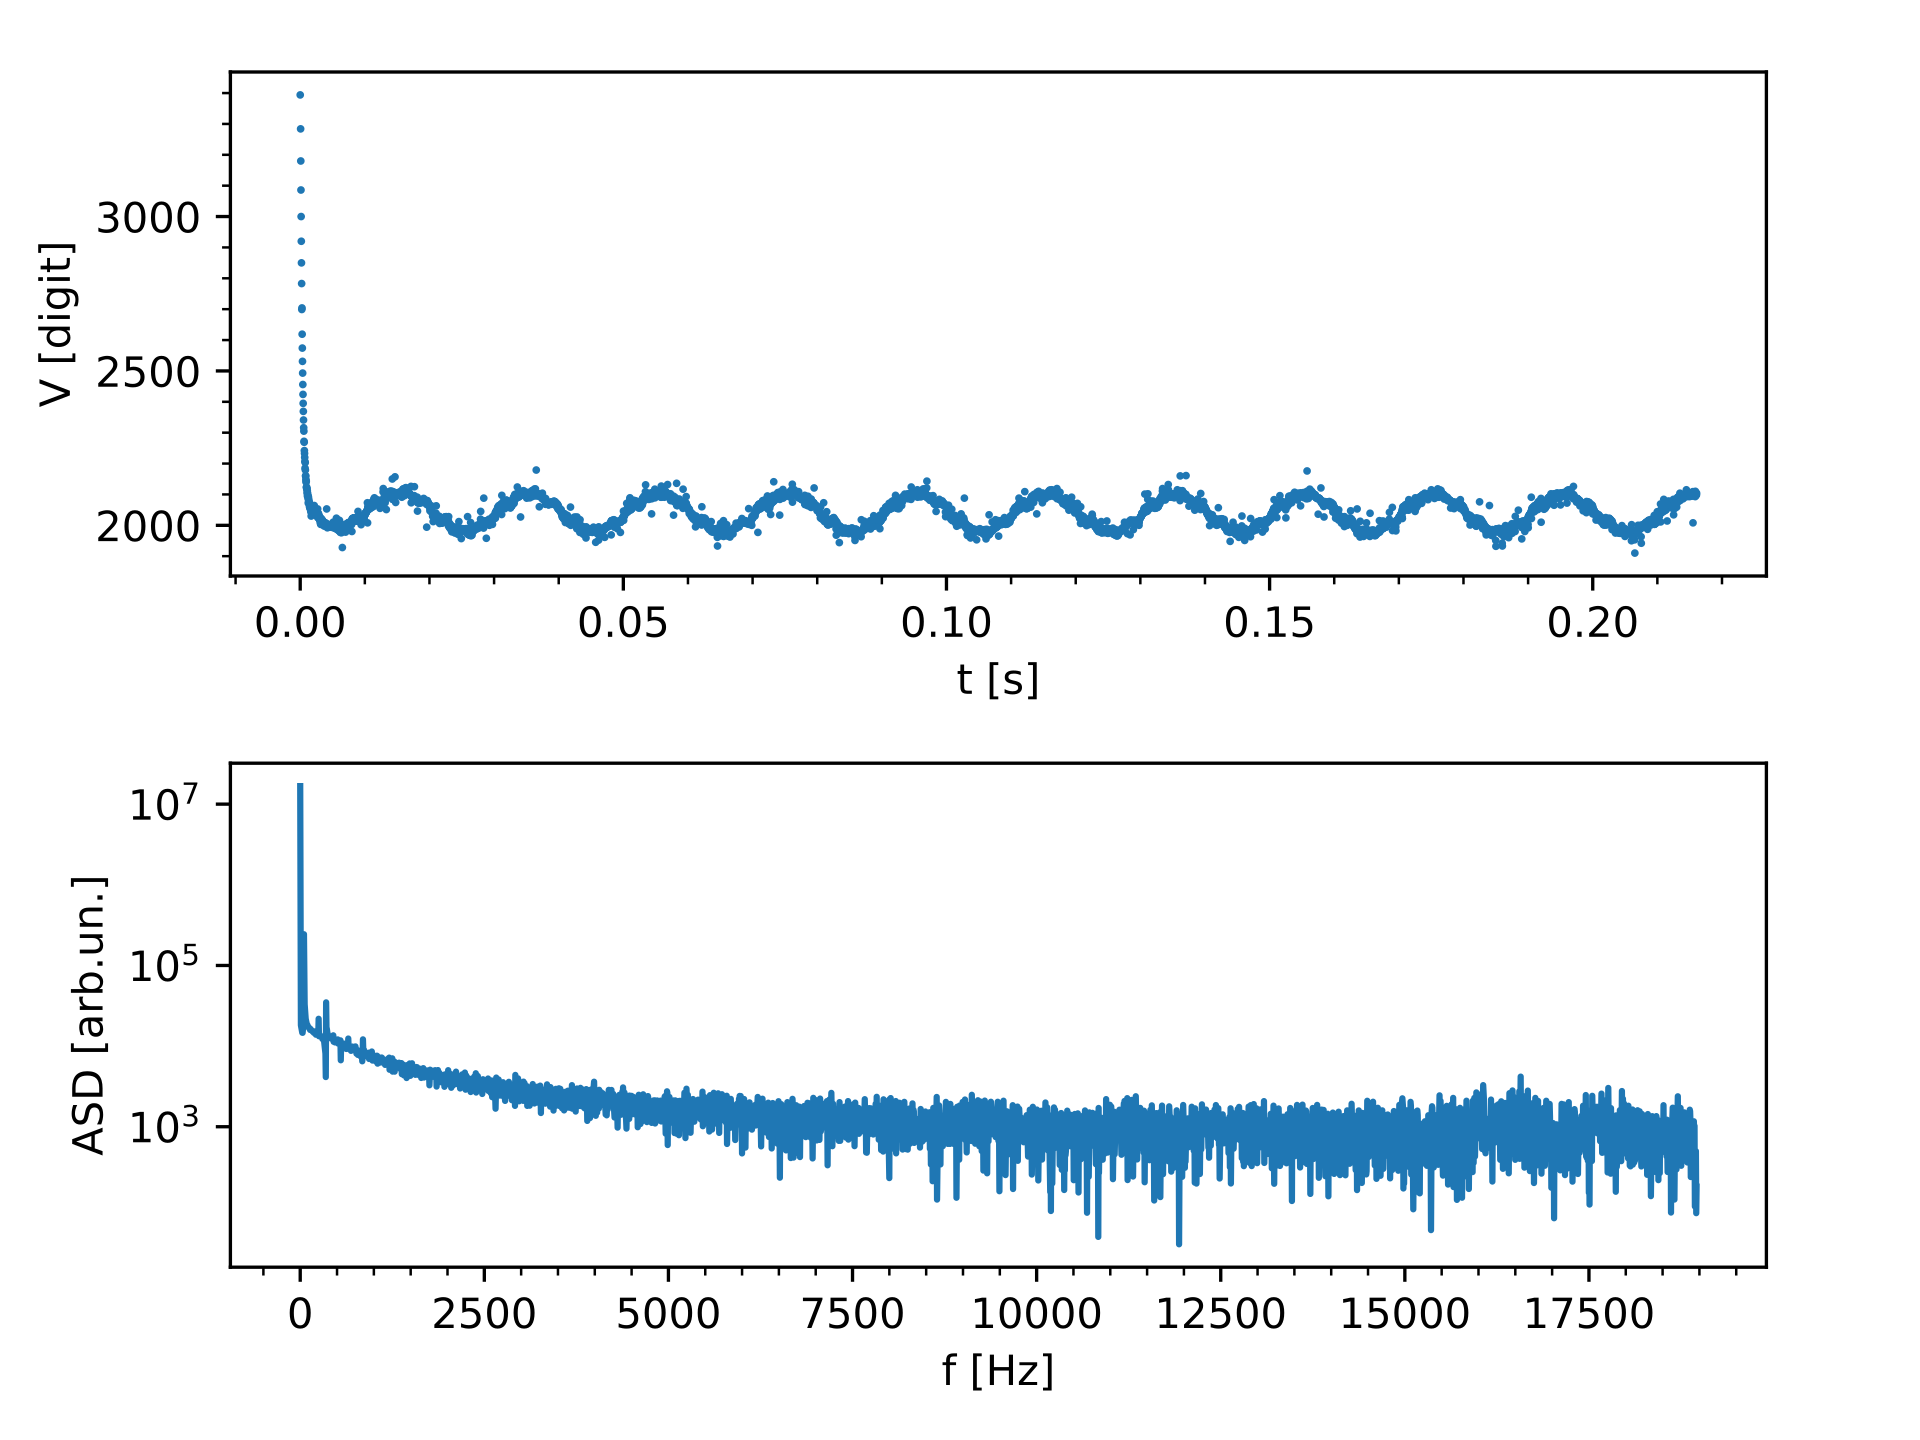
\includegraphics[width=0.45\columnwidth]{img/ese3/quanada}
    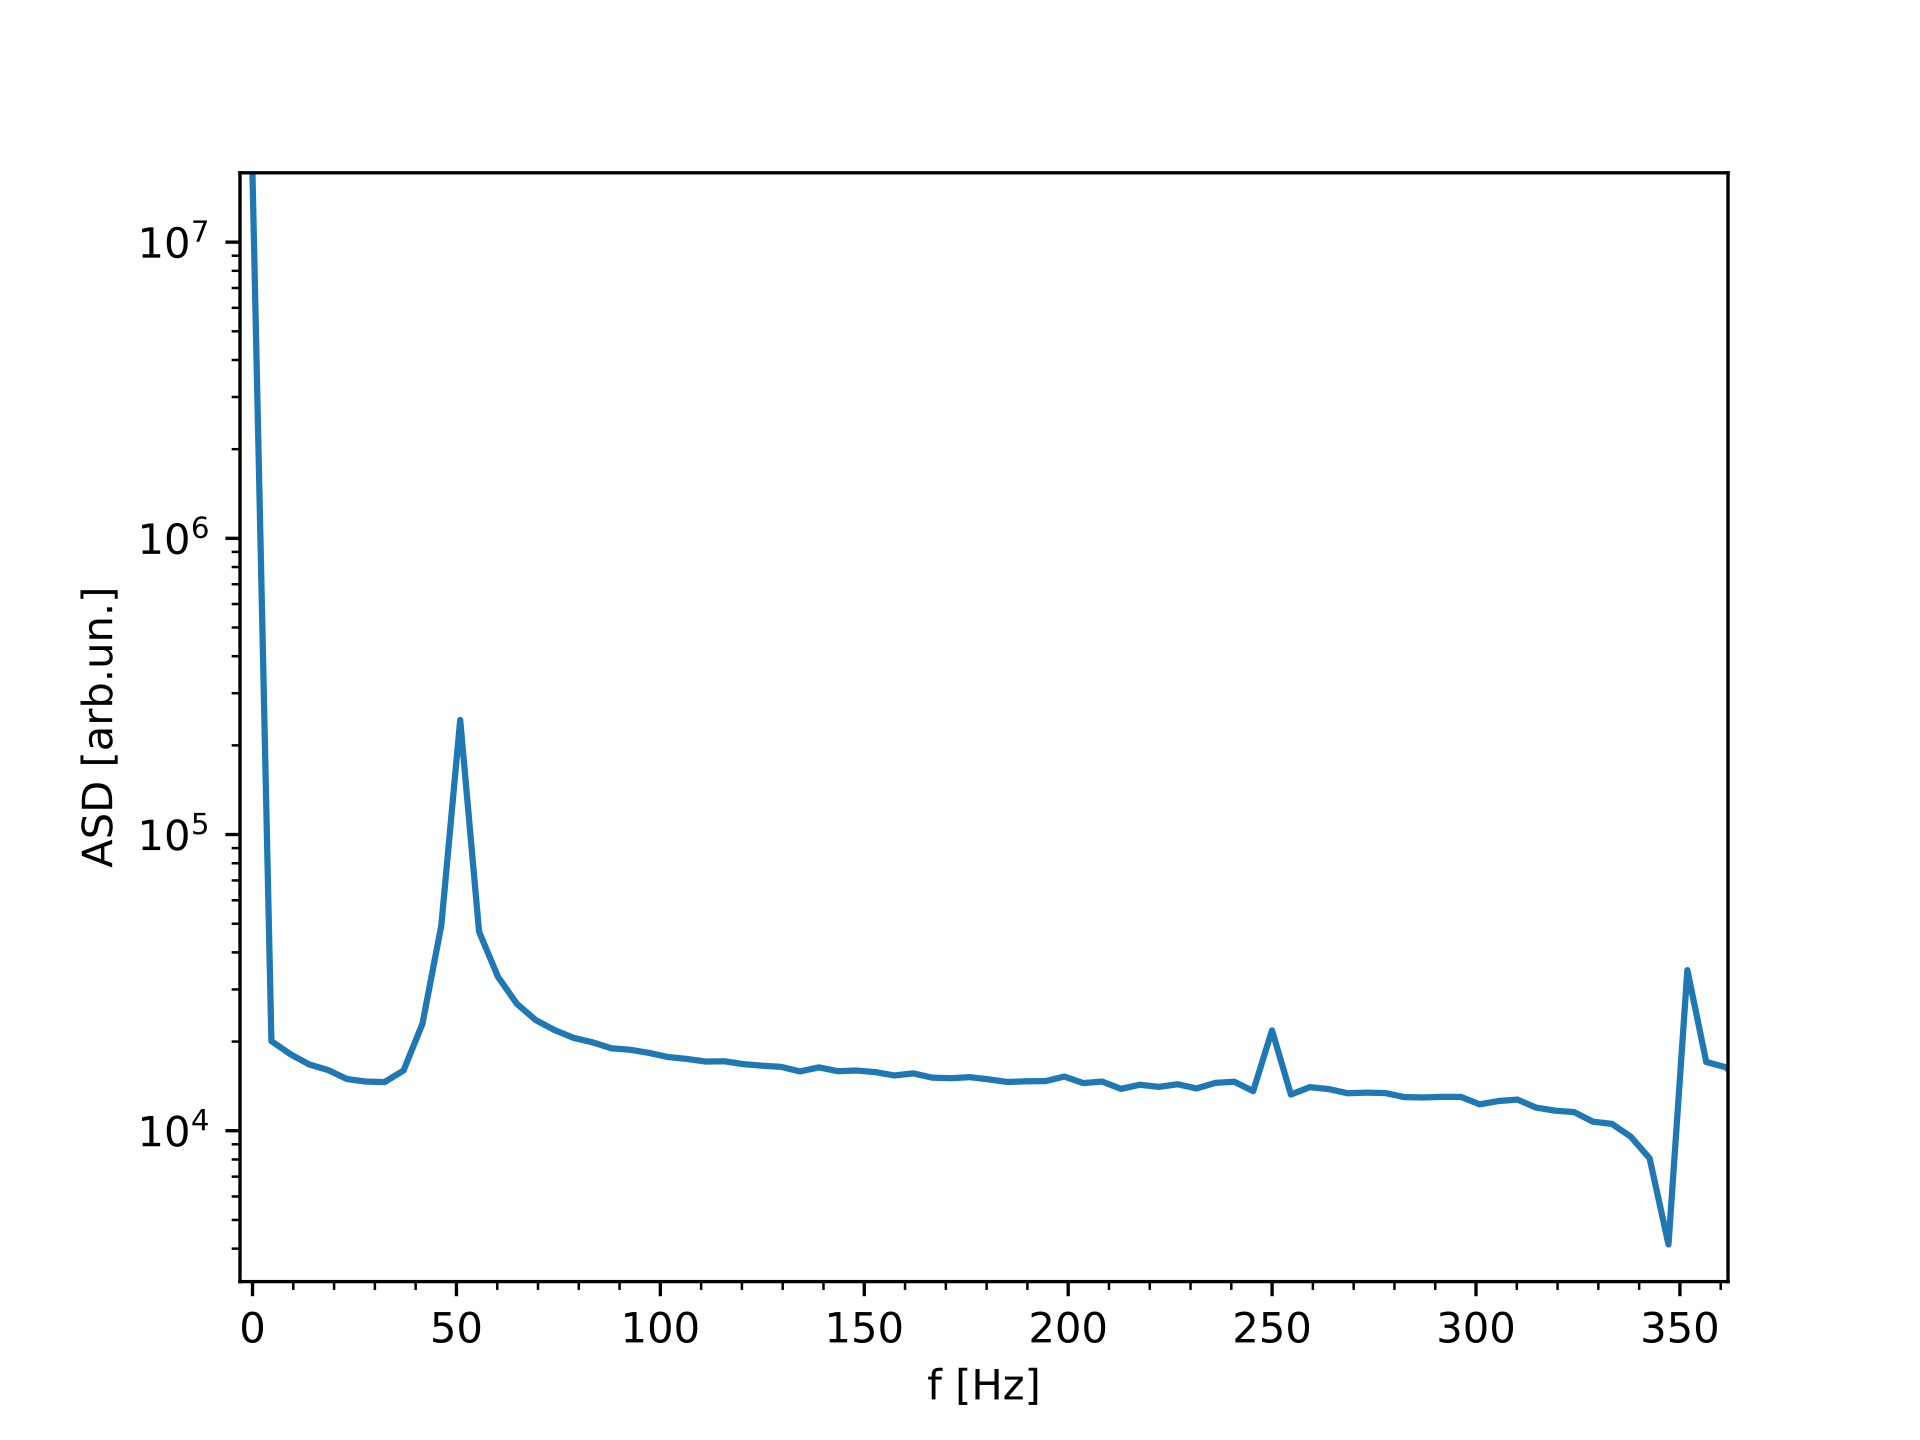
\includegraphics[width=0.48\columnwidth]{img/ese3/quanada-tagliato}
    \caption{Dati, FFT e zoom della FFT attorno alle basse frequenze per l'acquisizione \texttt{quanada.txt}}
    \label{fig:ese3-quanada}
\end{figure}

\begin{figure}[H]
    \centering
    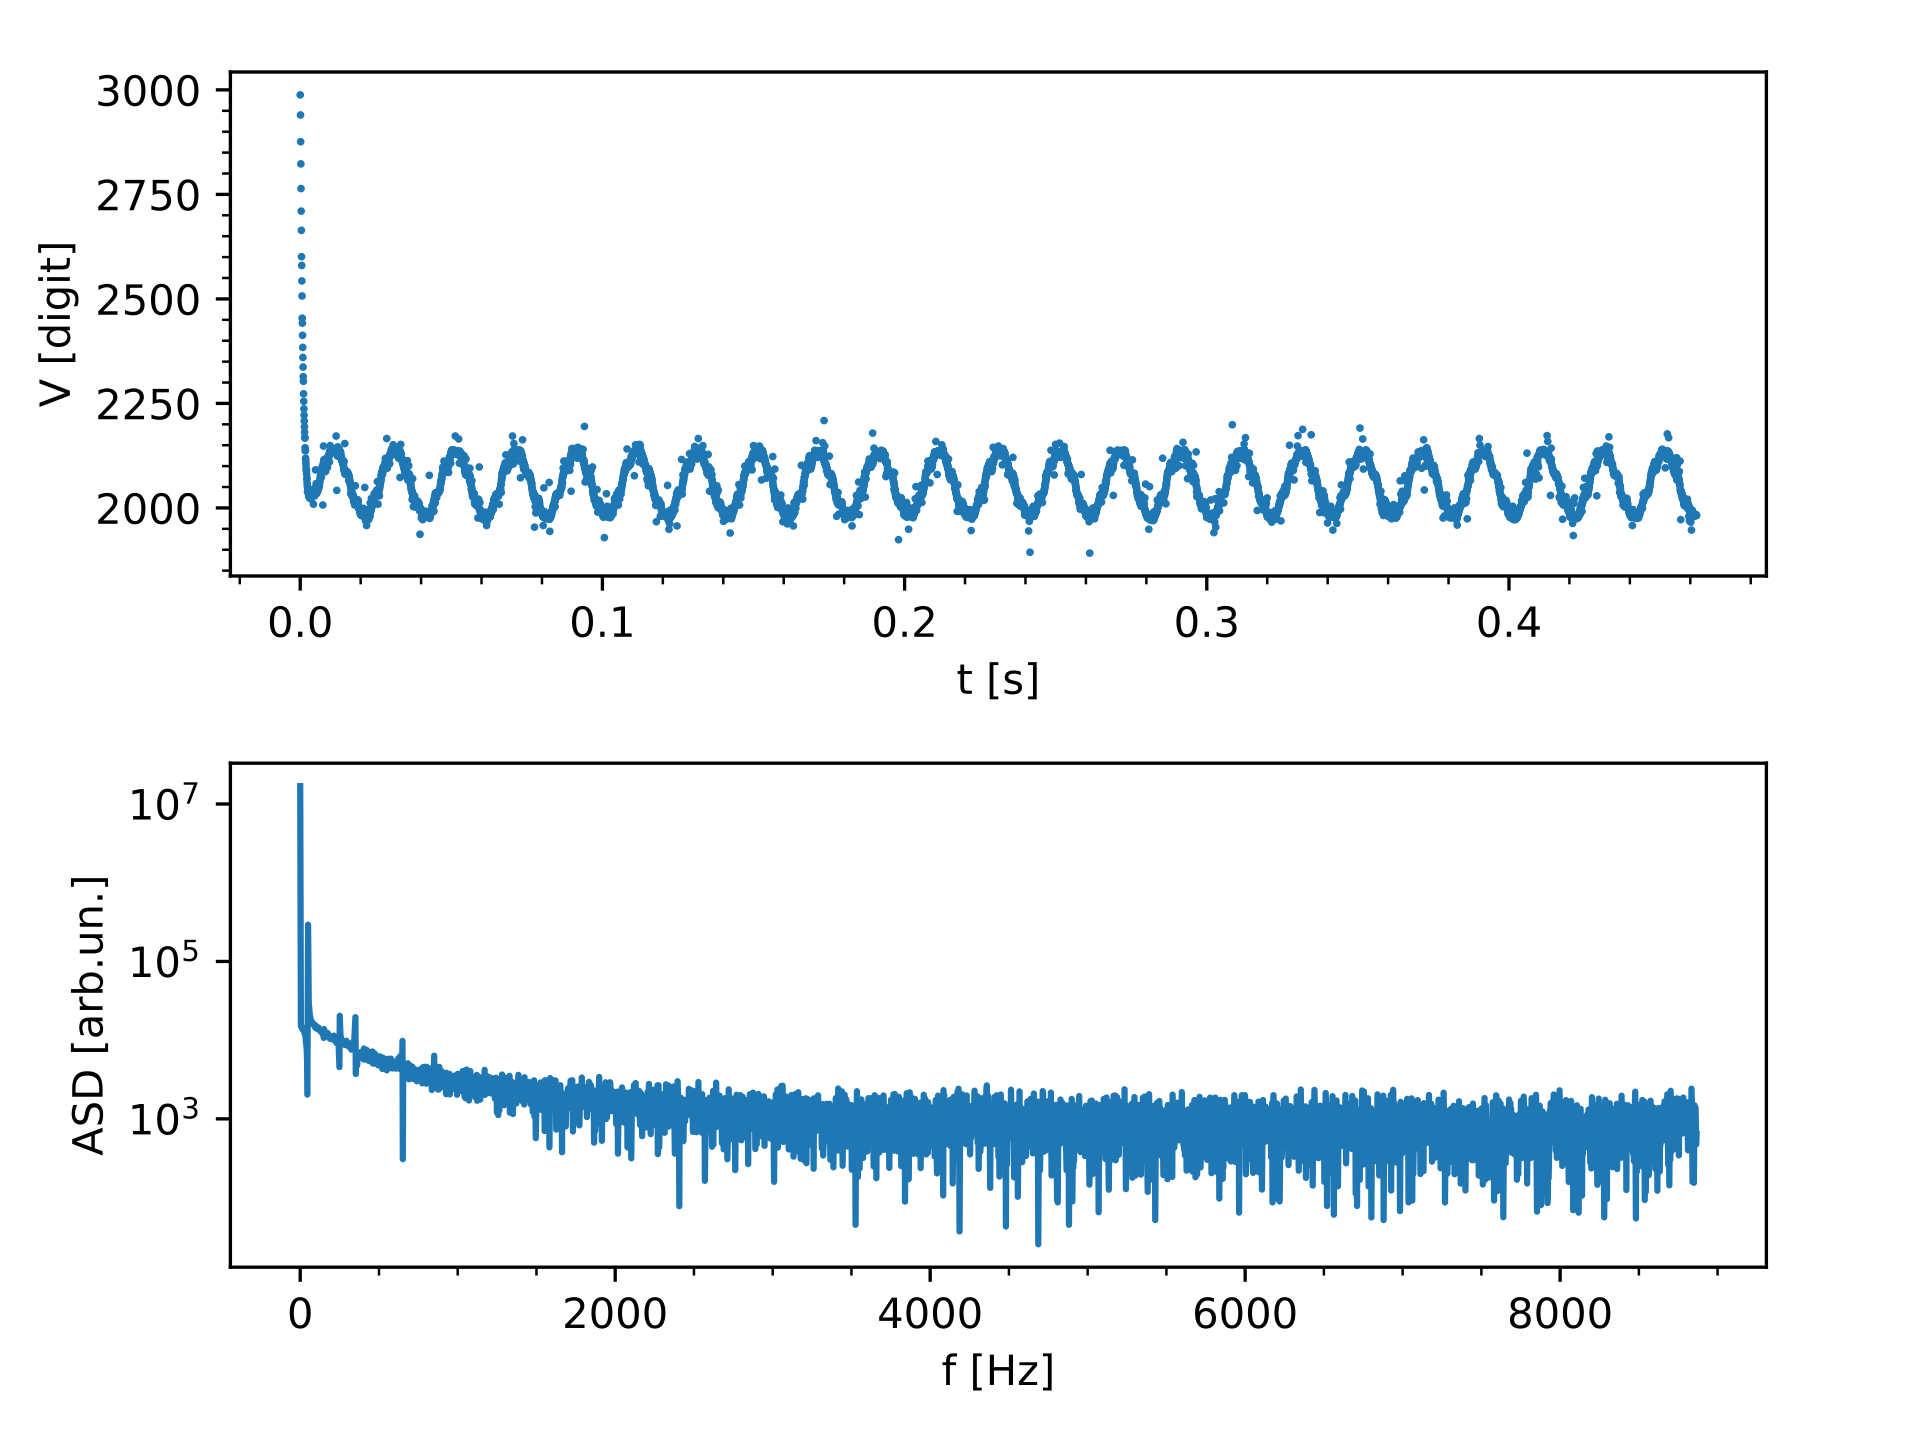
\includegraphics[width=0.45\columnwidth]{img/ese3/quinada}
    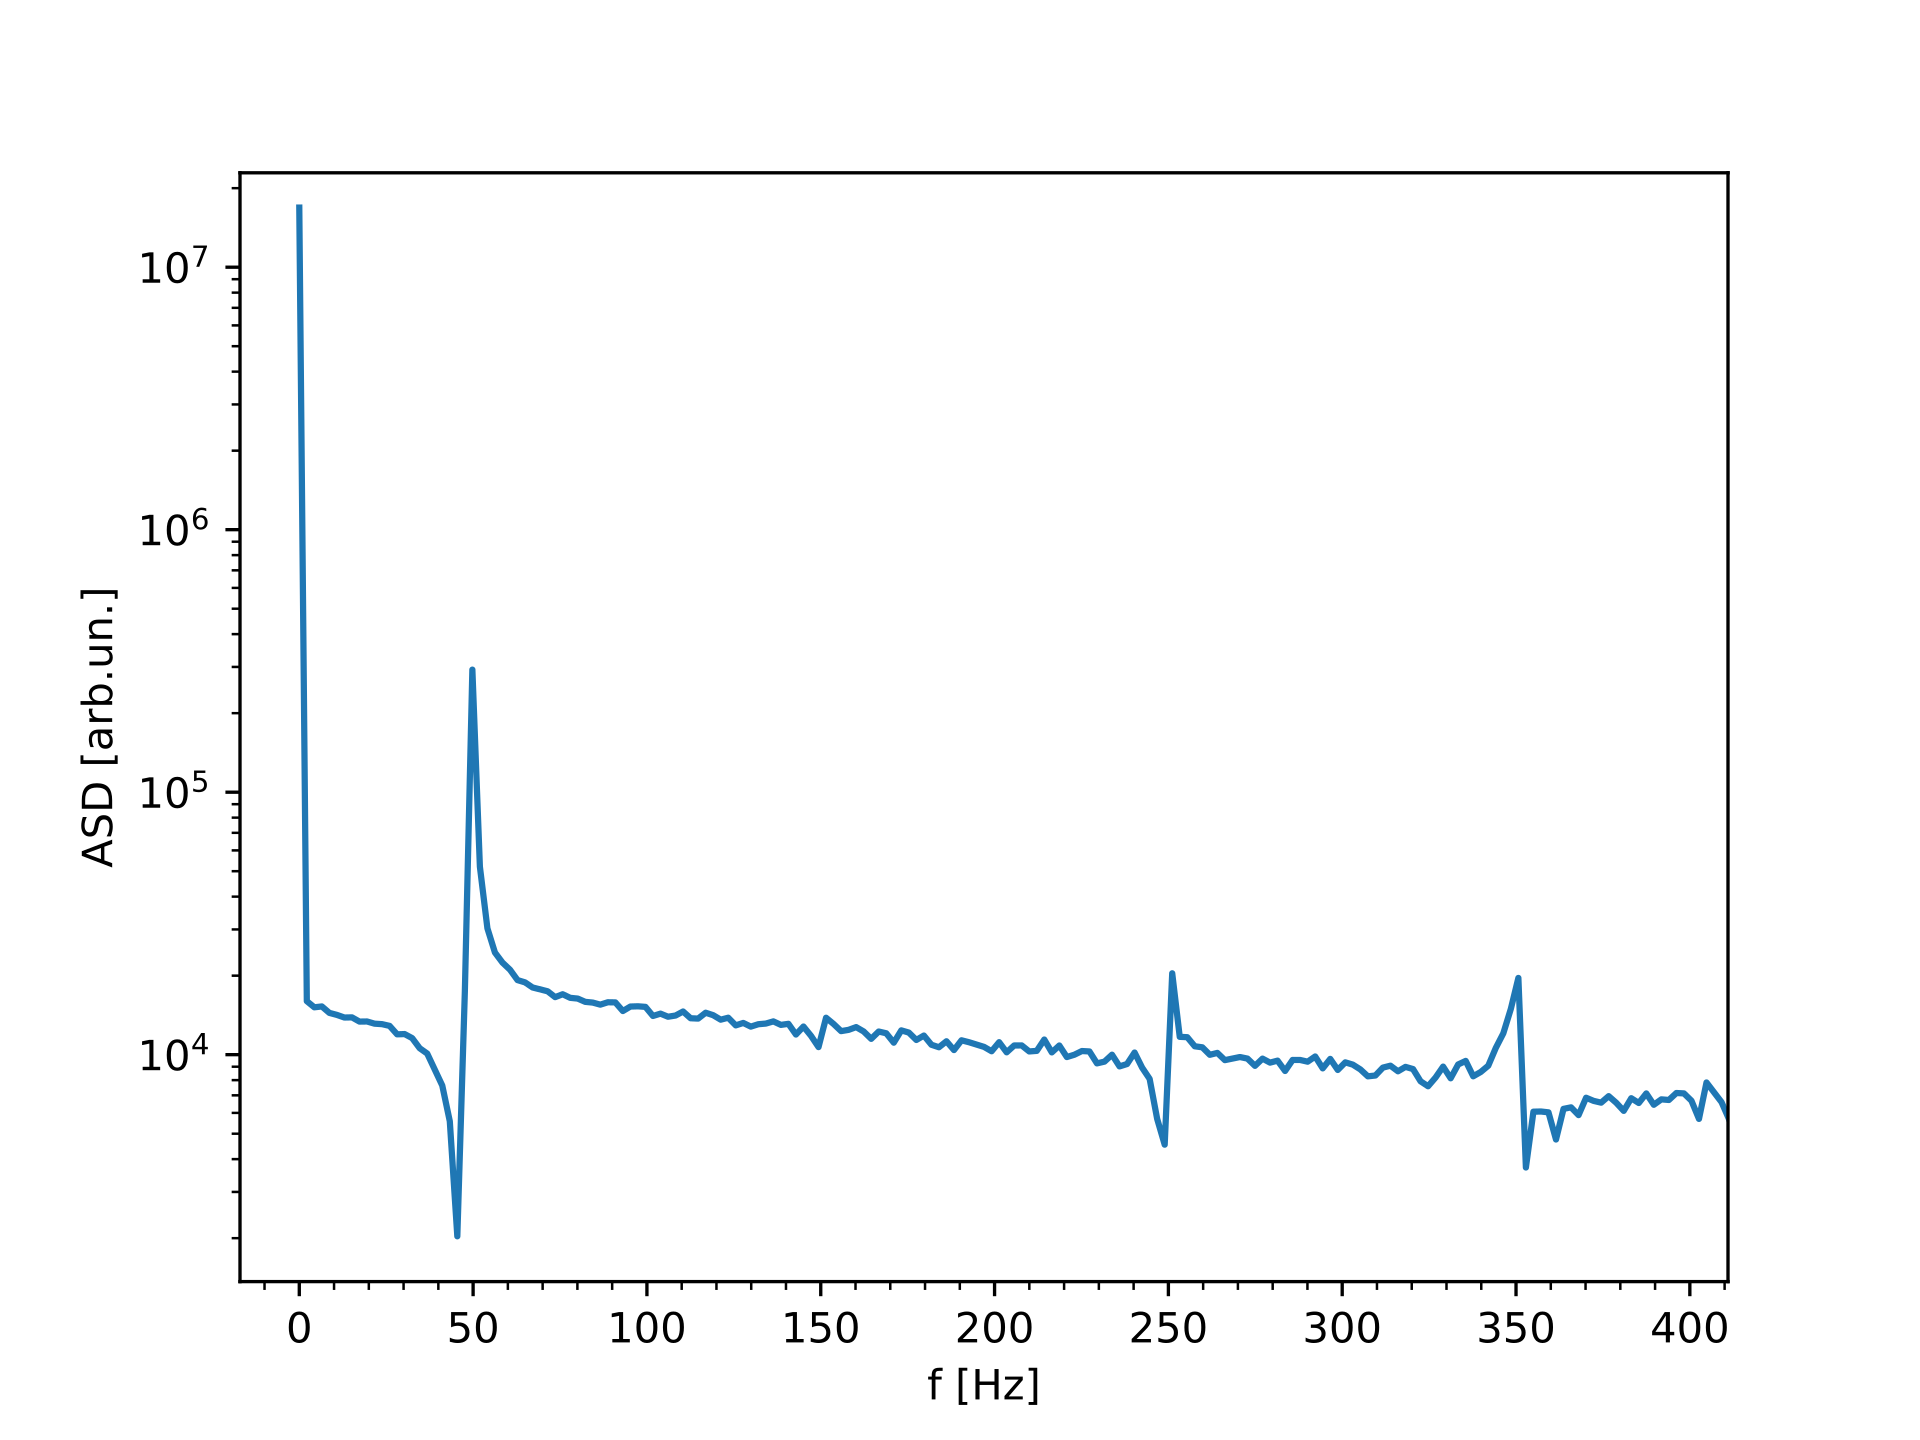
\includegraphics[width=0.48\columnwidth]{img/ese3/quinada-tagliato}
    \caption{Dati, FFT e zoom della FFT attorno alle basse frequenze per l'acquisizione \texttt{quinada.txt}}
    \label{fig:ese3-quinada}
\end{figure}


\section{Alcune forme d'onda}
Abbiamo graficato i dati acquisiti collegando Arduino direttamente al generatore di forme d'onda, configurato in varie modalità.\\
Abbiamo acquisito per due diverse frequenze forme d'onda sinusoidali, triangolari e quadre: queste ultime anche con \textit{duty cycle} massimo consentito dal generatore in entrambe le direzioni. \\
Notiamo che in tutti i casi è presente un picco alla frequenza dell'onda e altri picchi minori in corrispondenza delle armoniche. Nel caso dell'onda sinusoidale ci aspetteremmo un unico picco molto concentrato attorno alla frequenza dell'onda. Per via di imperfezioni del generatore reale e effetti dovuti al campionamento e alla digitalizzazione, possono però comparire delle armoniche. I picchi che osserviamo in corrispondenza di tali frequenze sono di ampiezza almeno due ordini di grandezza inferiori alla fondamentale, quindi comunque molto minori di quanto invece osserviamo nelle altre due forme d'onda.\\
Per le onde triangolari e quadre invece ci aspetteremmo che le armoniche presentino lo stesso andamento dei coefficienti della serie di Fourier per tali forme d'onda. Per tale motivo abbiamo realizzato grafici aggiuntivi in cui abbiamo rappresentato la curva corrispondente ad una legge di potenza che meglio approssimasse i picchi delle armoniche.\\
Nel caso dell'onda quadra abbiamo notato che i picchi seguono un andamento del tipo $n^{-1.06}$, invece che $n^{-1}$. Questo valore dell'esponente fitta anche i dati della sezione successiva, per cui è probabilmente dovuto ad al rumore (vedi sezione 5).

\begin{figure}[H]
    \centering
    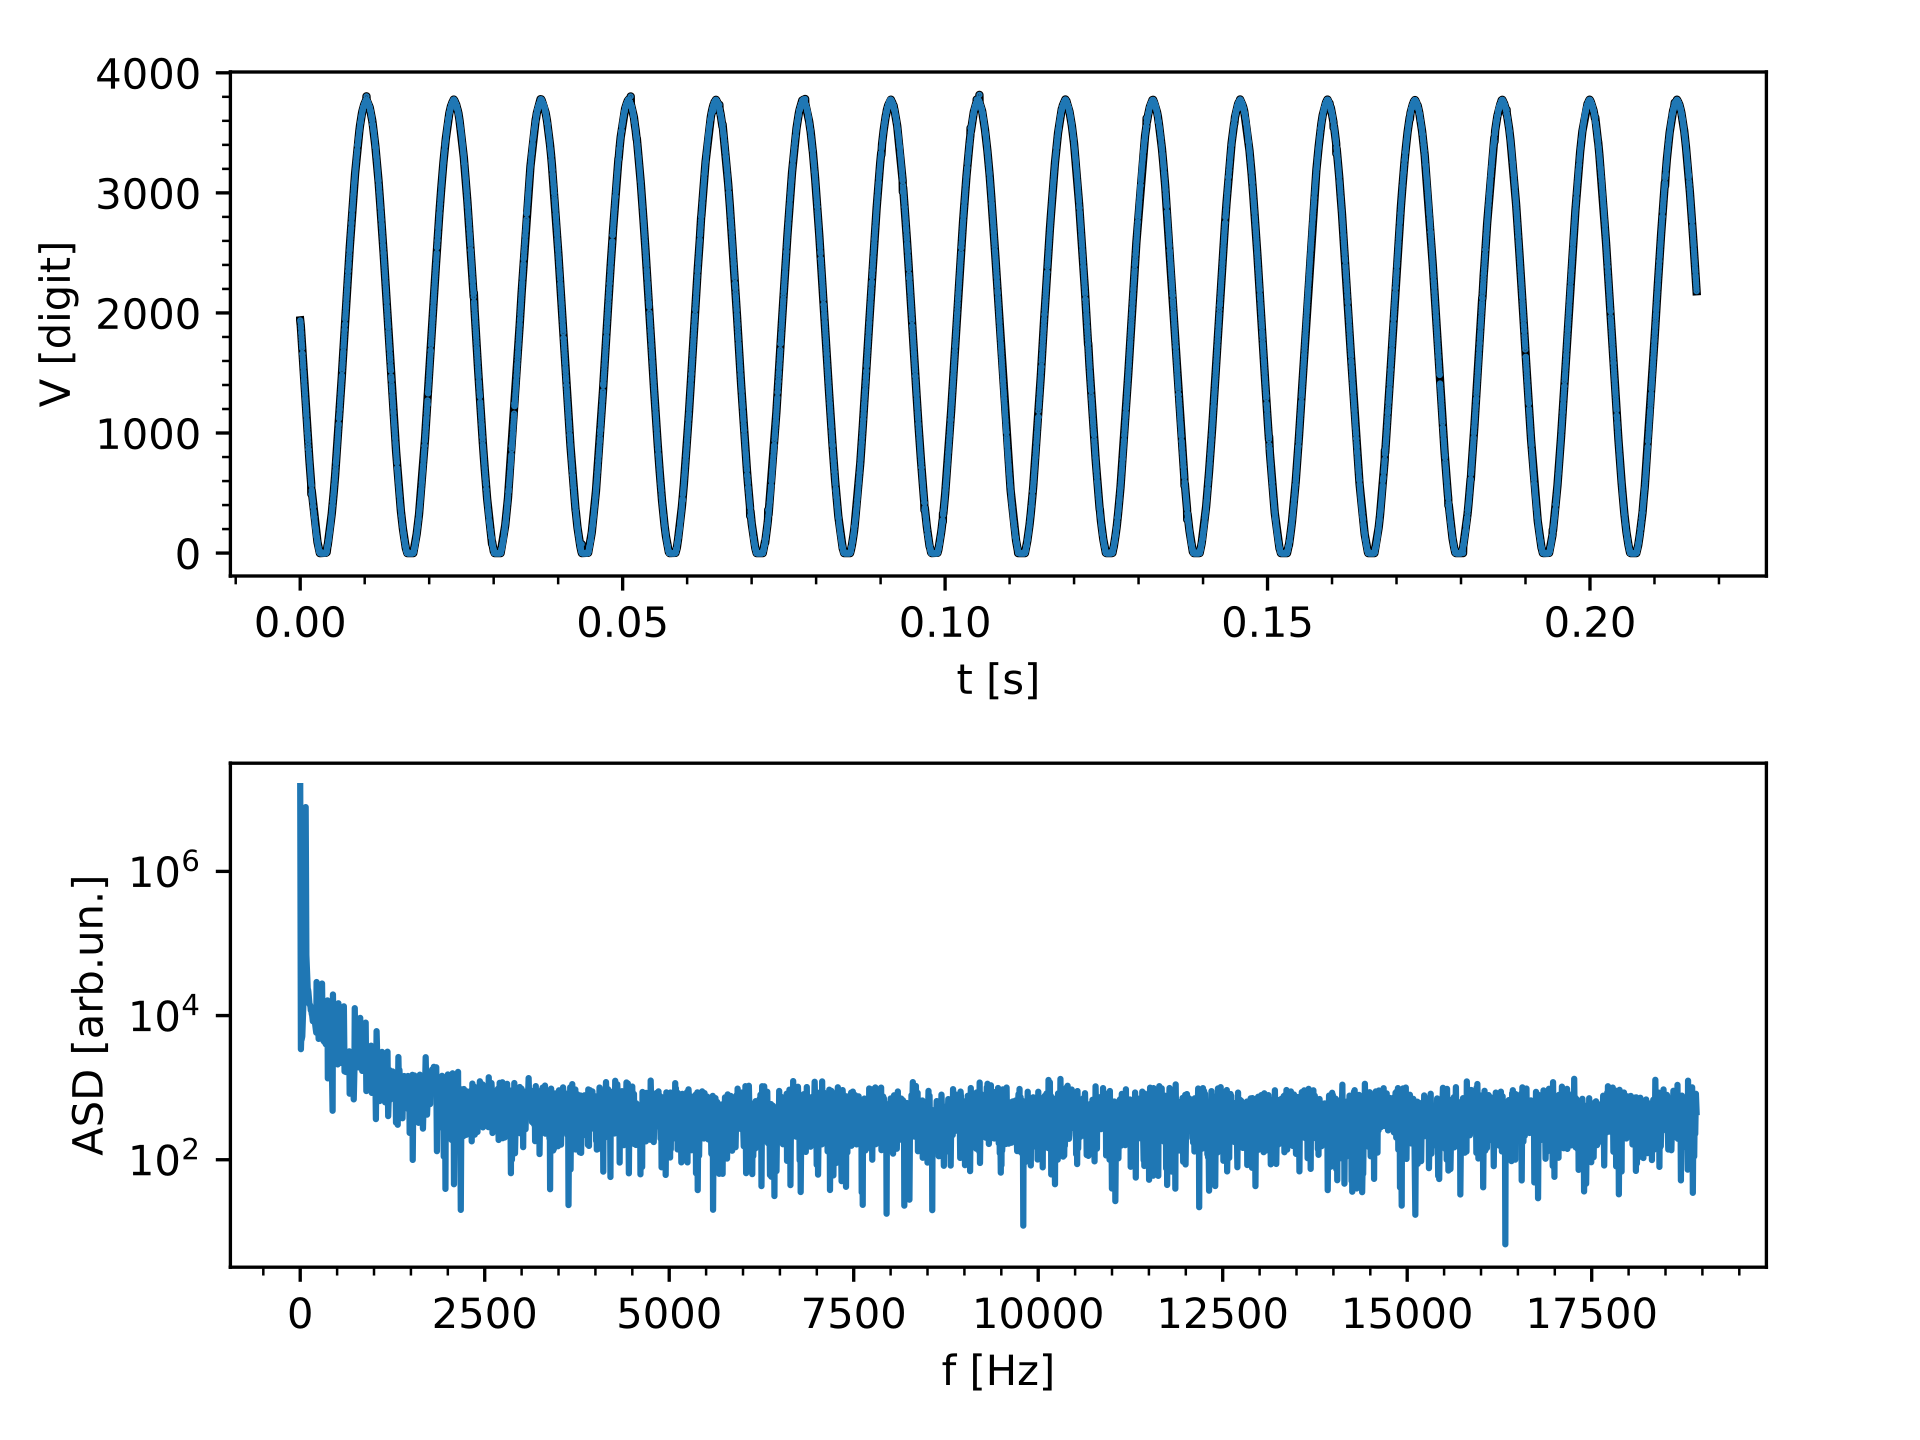
\includegraphics[width=0.45\columnwidth]{img/ese5/f73_SN}
    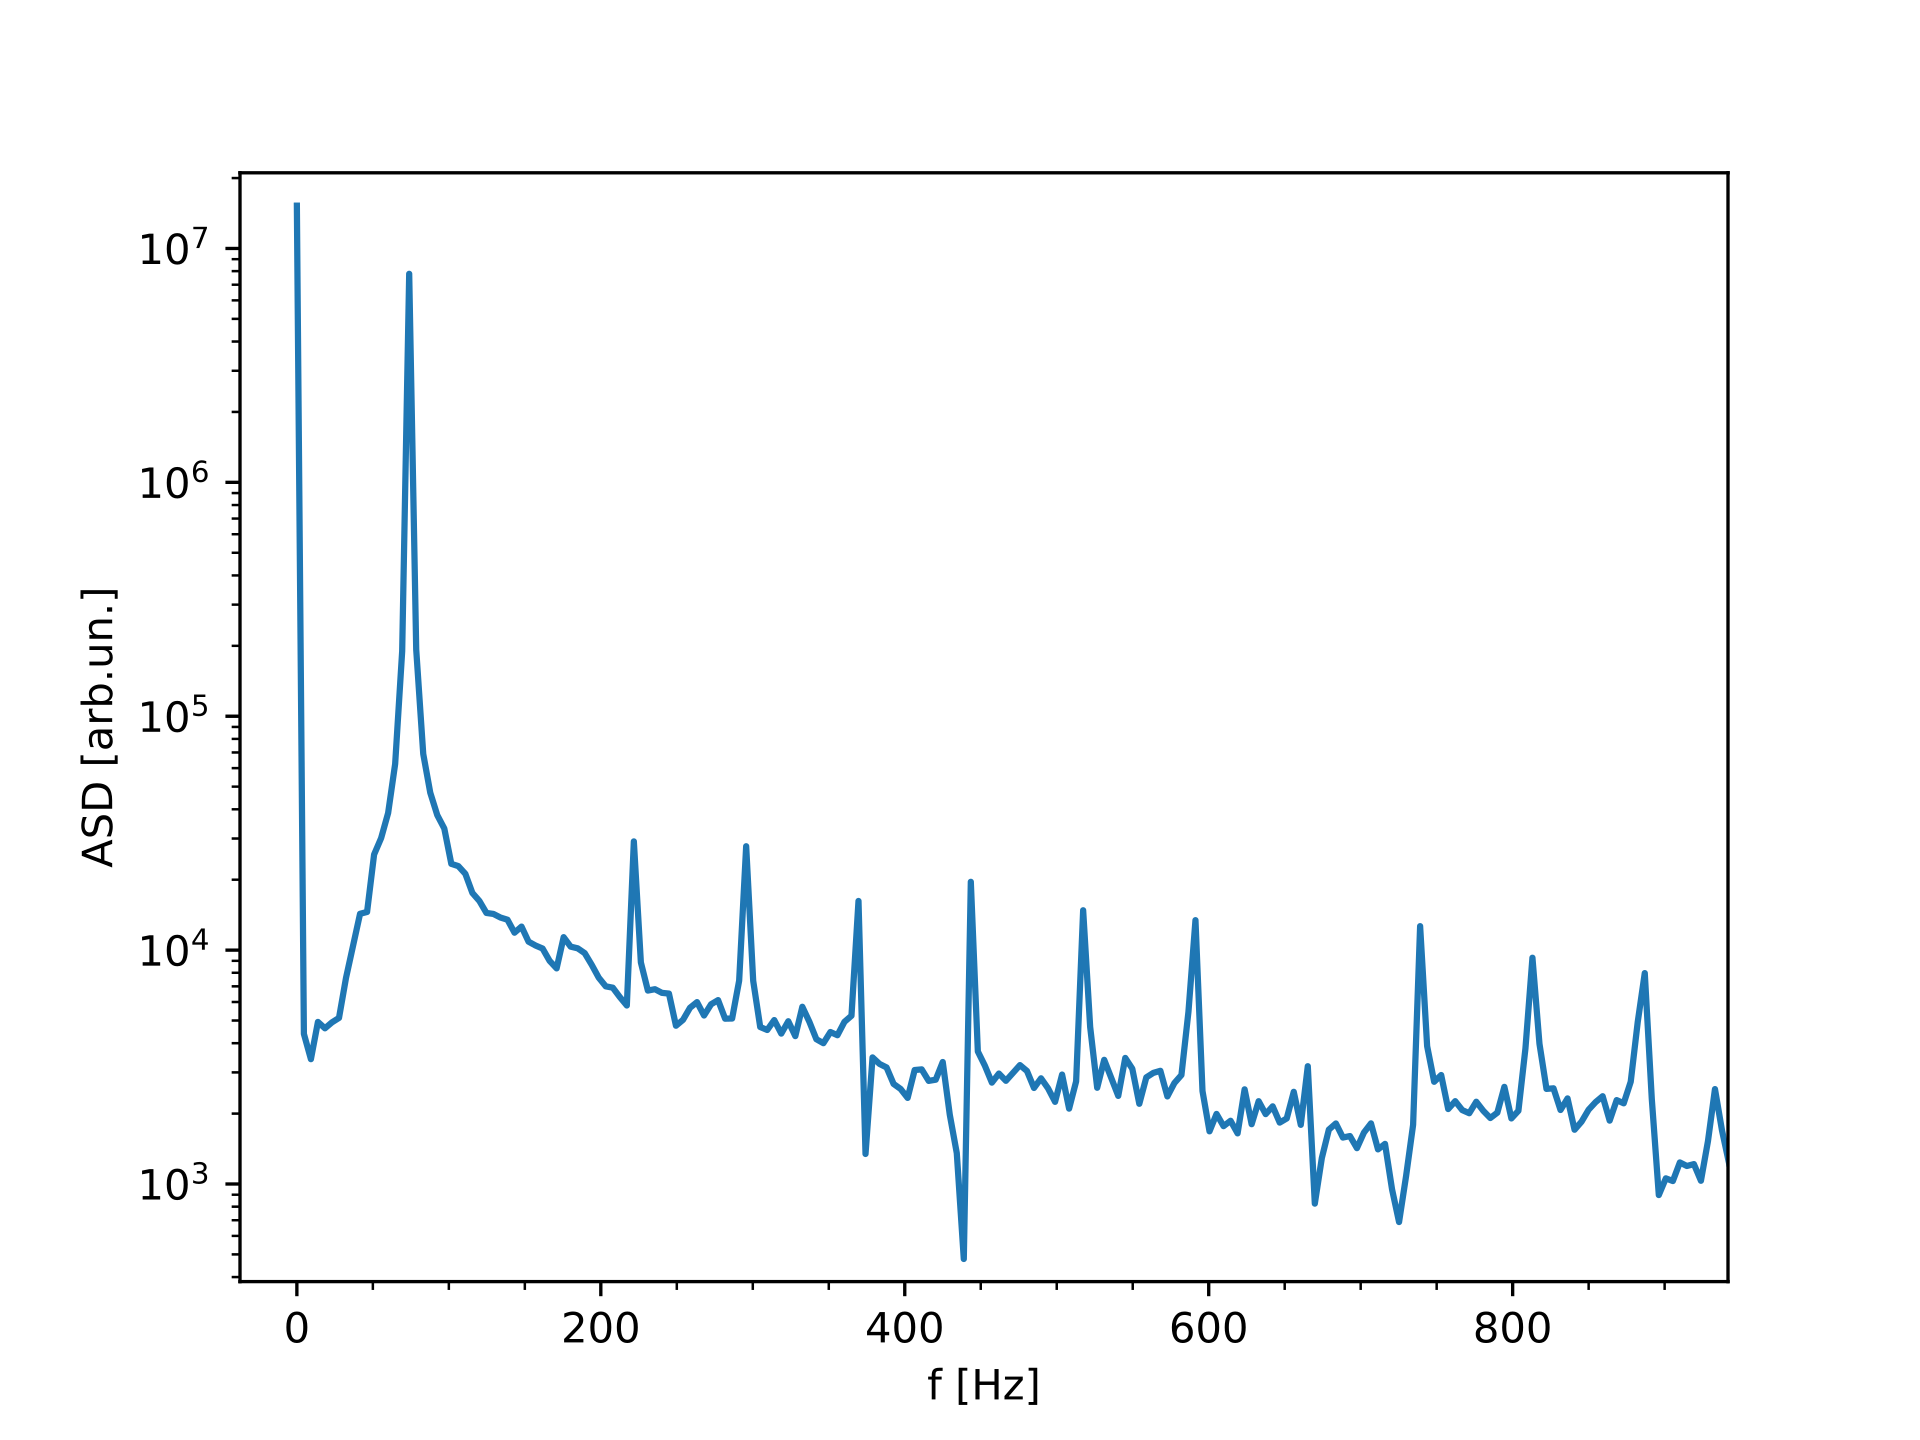
\includegraphics[width=0.48\columnwidth]{img/ese5/f73_SN-tagl}
    \caption{Grafici relativi ad un'onda sinusoidale a frequenza (73.246 $\pm$ 0.001) Hz. Notare i picchi in corrispondenza delle armoniche di ampiezza di 2-3 ordini di grandezza inferiori rispetto alla fondamentale.}
    \label{fig:ese5-f73_SN}
\end{figure}

\begin{figure}[H]
    \centering
    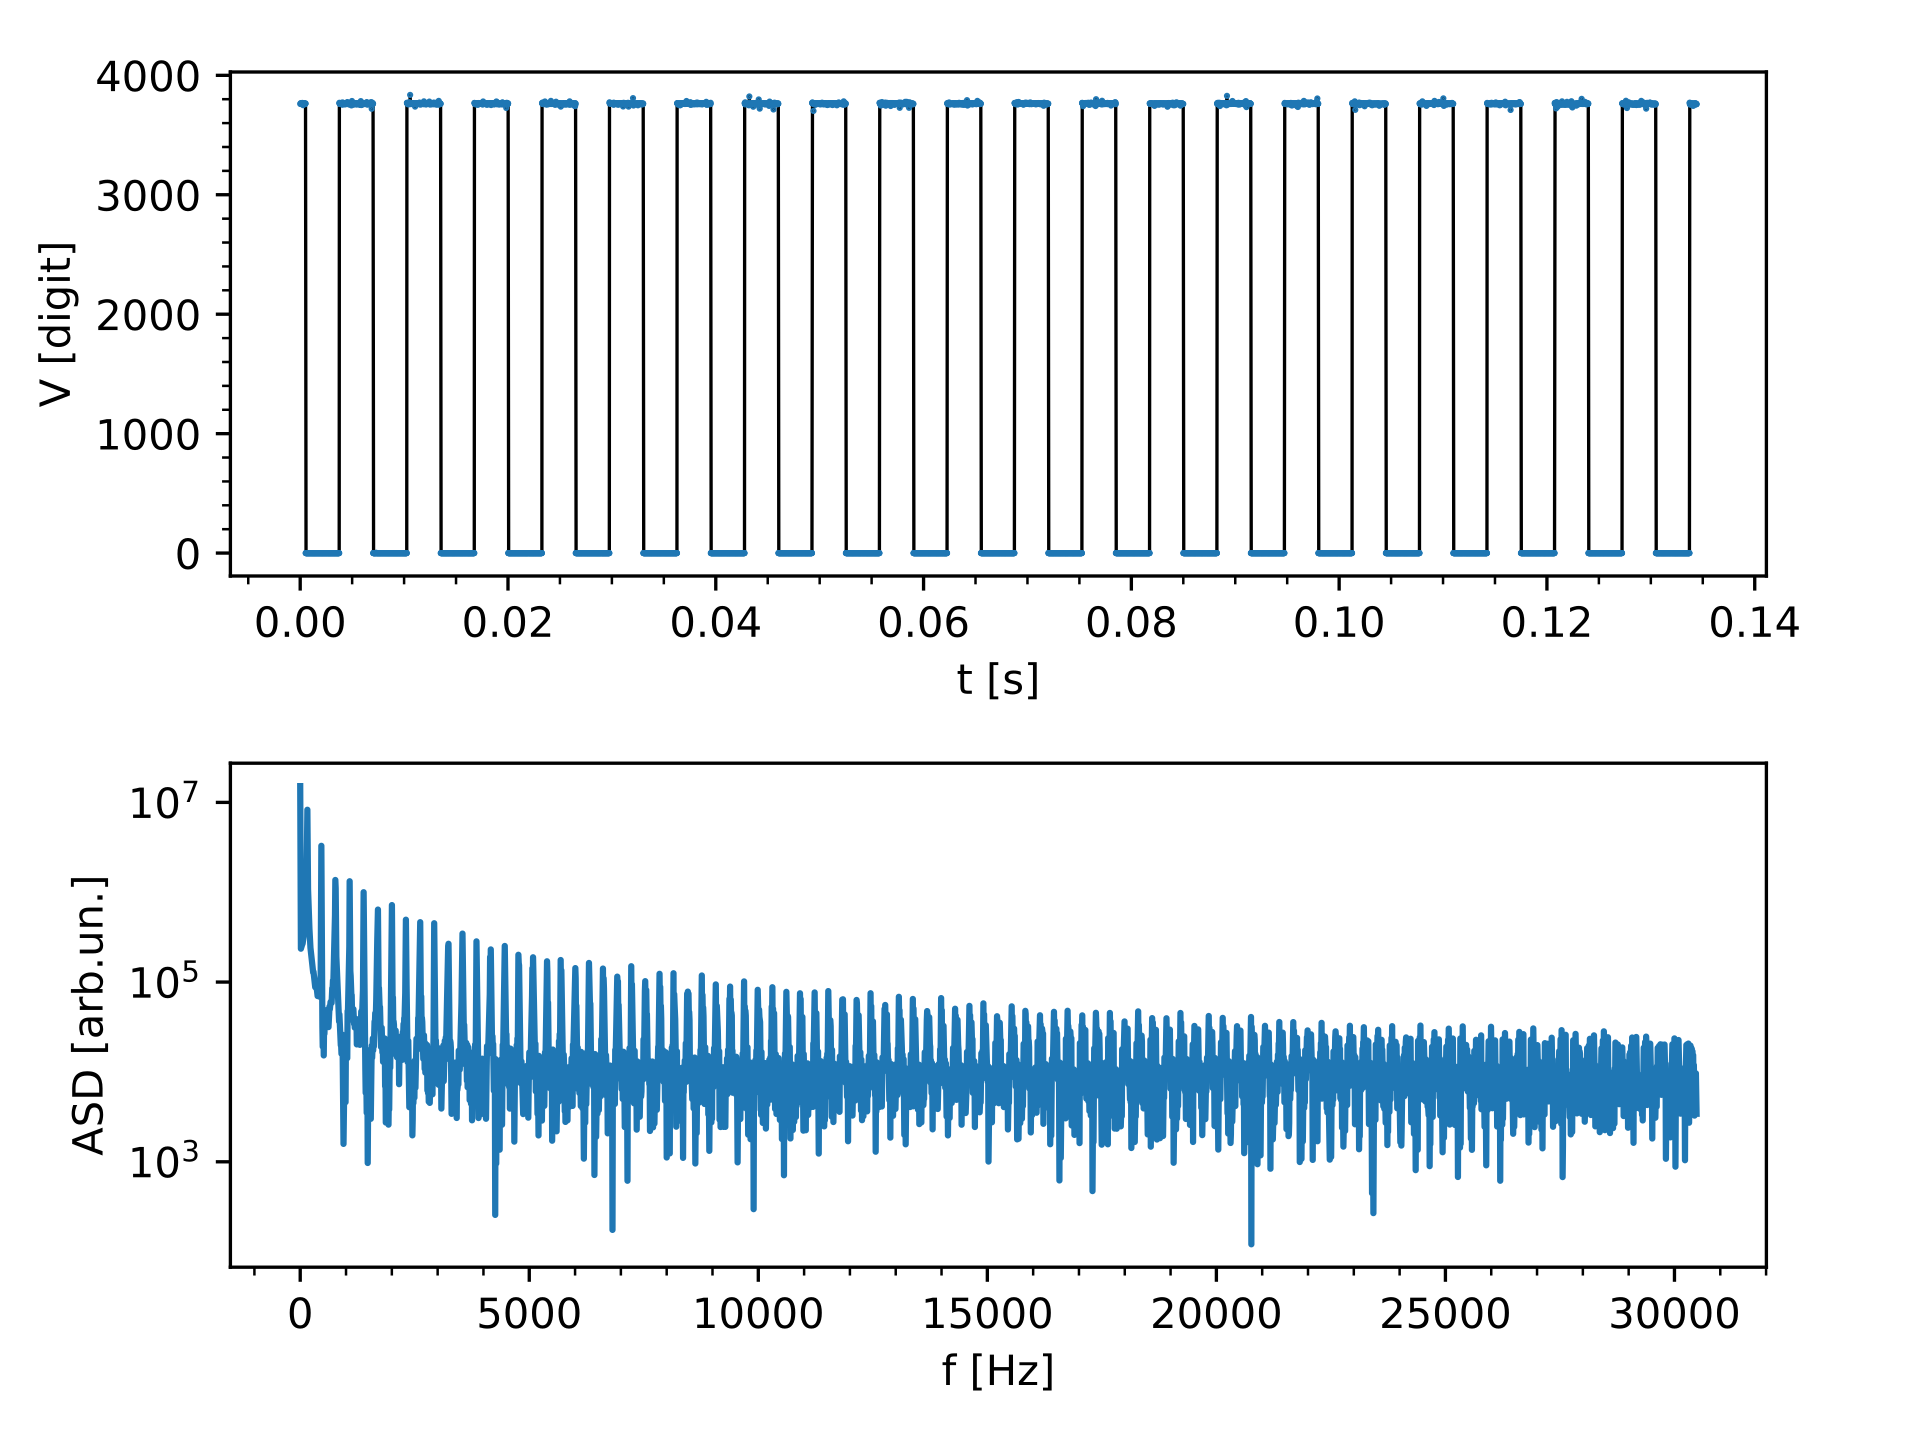
\includegraphics[width=0.45\columnwidth]{img/ese5/f153_QN}
    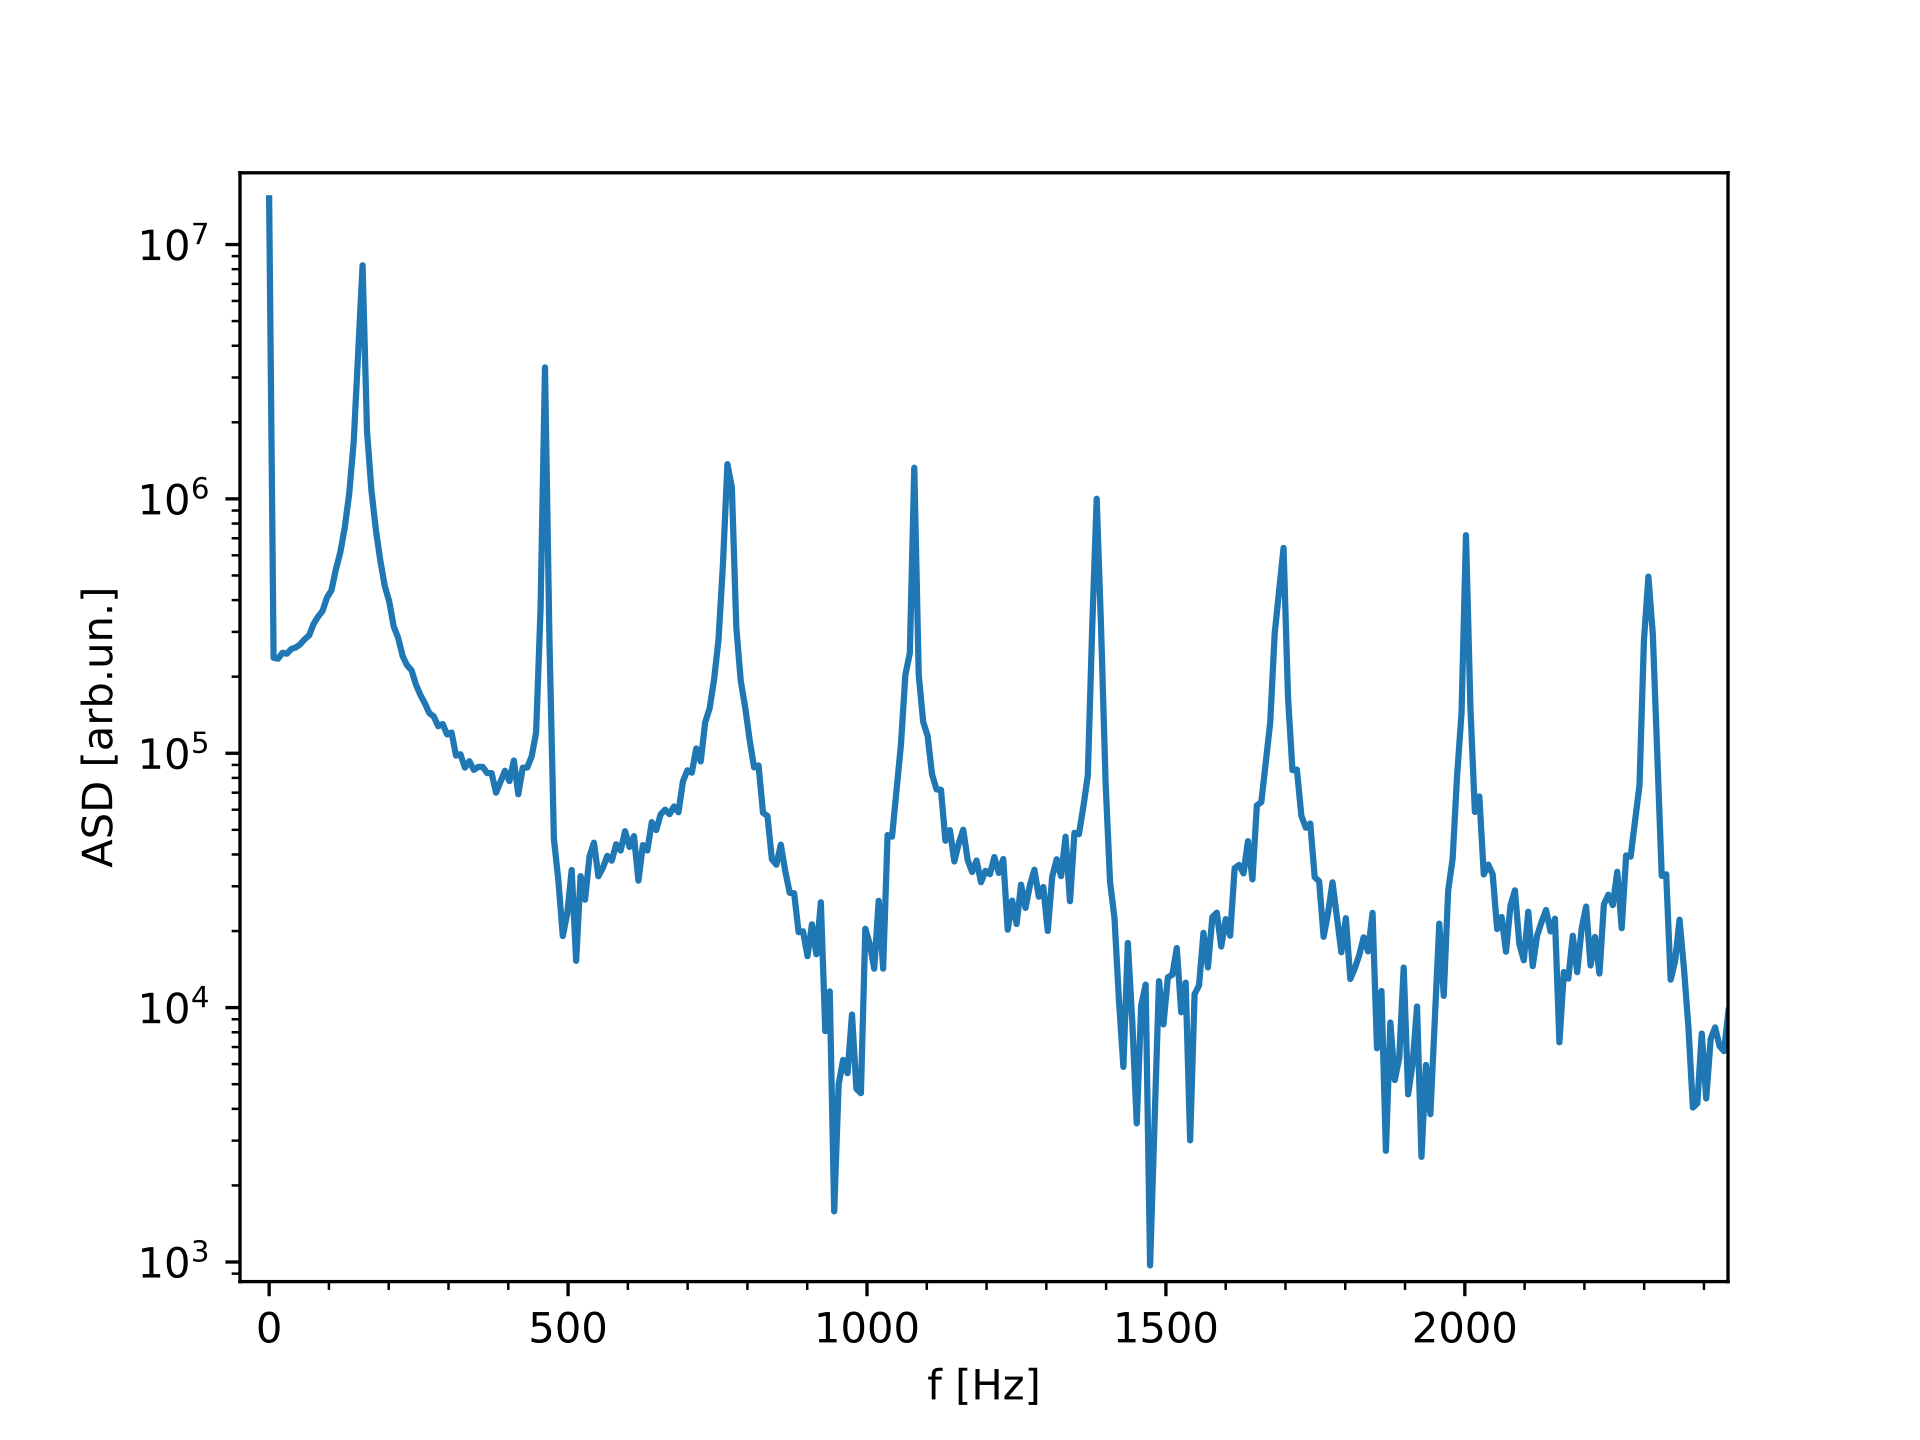
\includegraphics[width=0.48\columnwidth]{img/ese5/f153_QN-tagl}
    \caption{Grafici relativi ad un'onda quadra a frequenza (153.77 $\pm$ 0.01) Hz. Notare i picchi in corrispondenza delle armoniche dispari.}
    \label{fig:ese5-f73_QN}
\end{figure}

\begin{figure}[H]
    \centering
    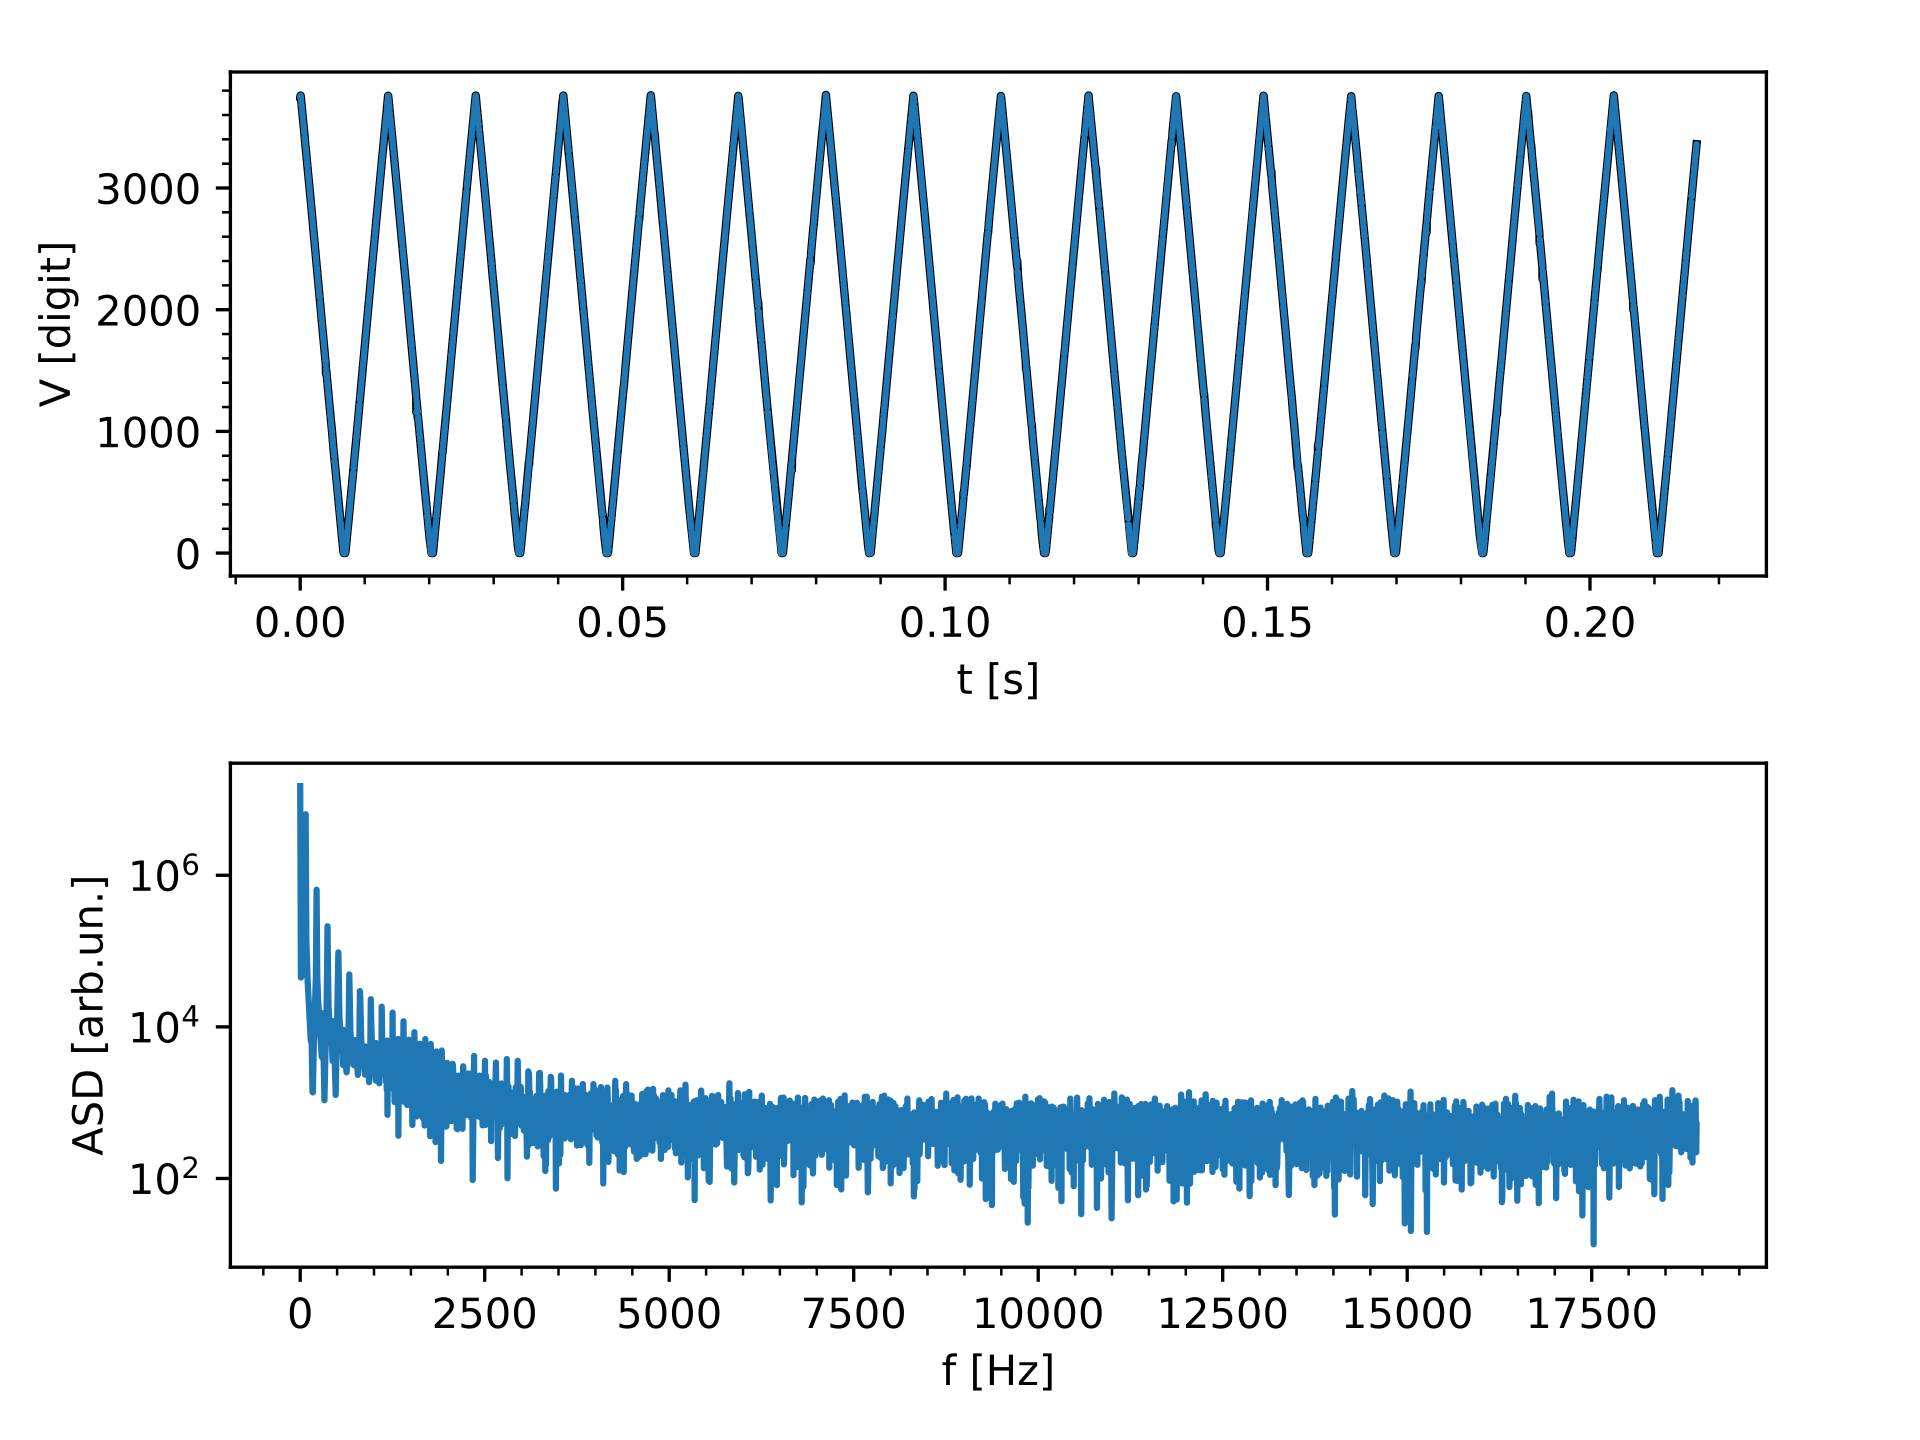
\includegraphics[width=0.45\columnwidth]{img/ese5/f73_TN}
    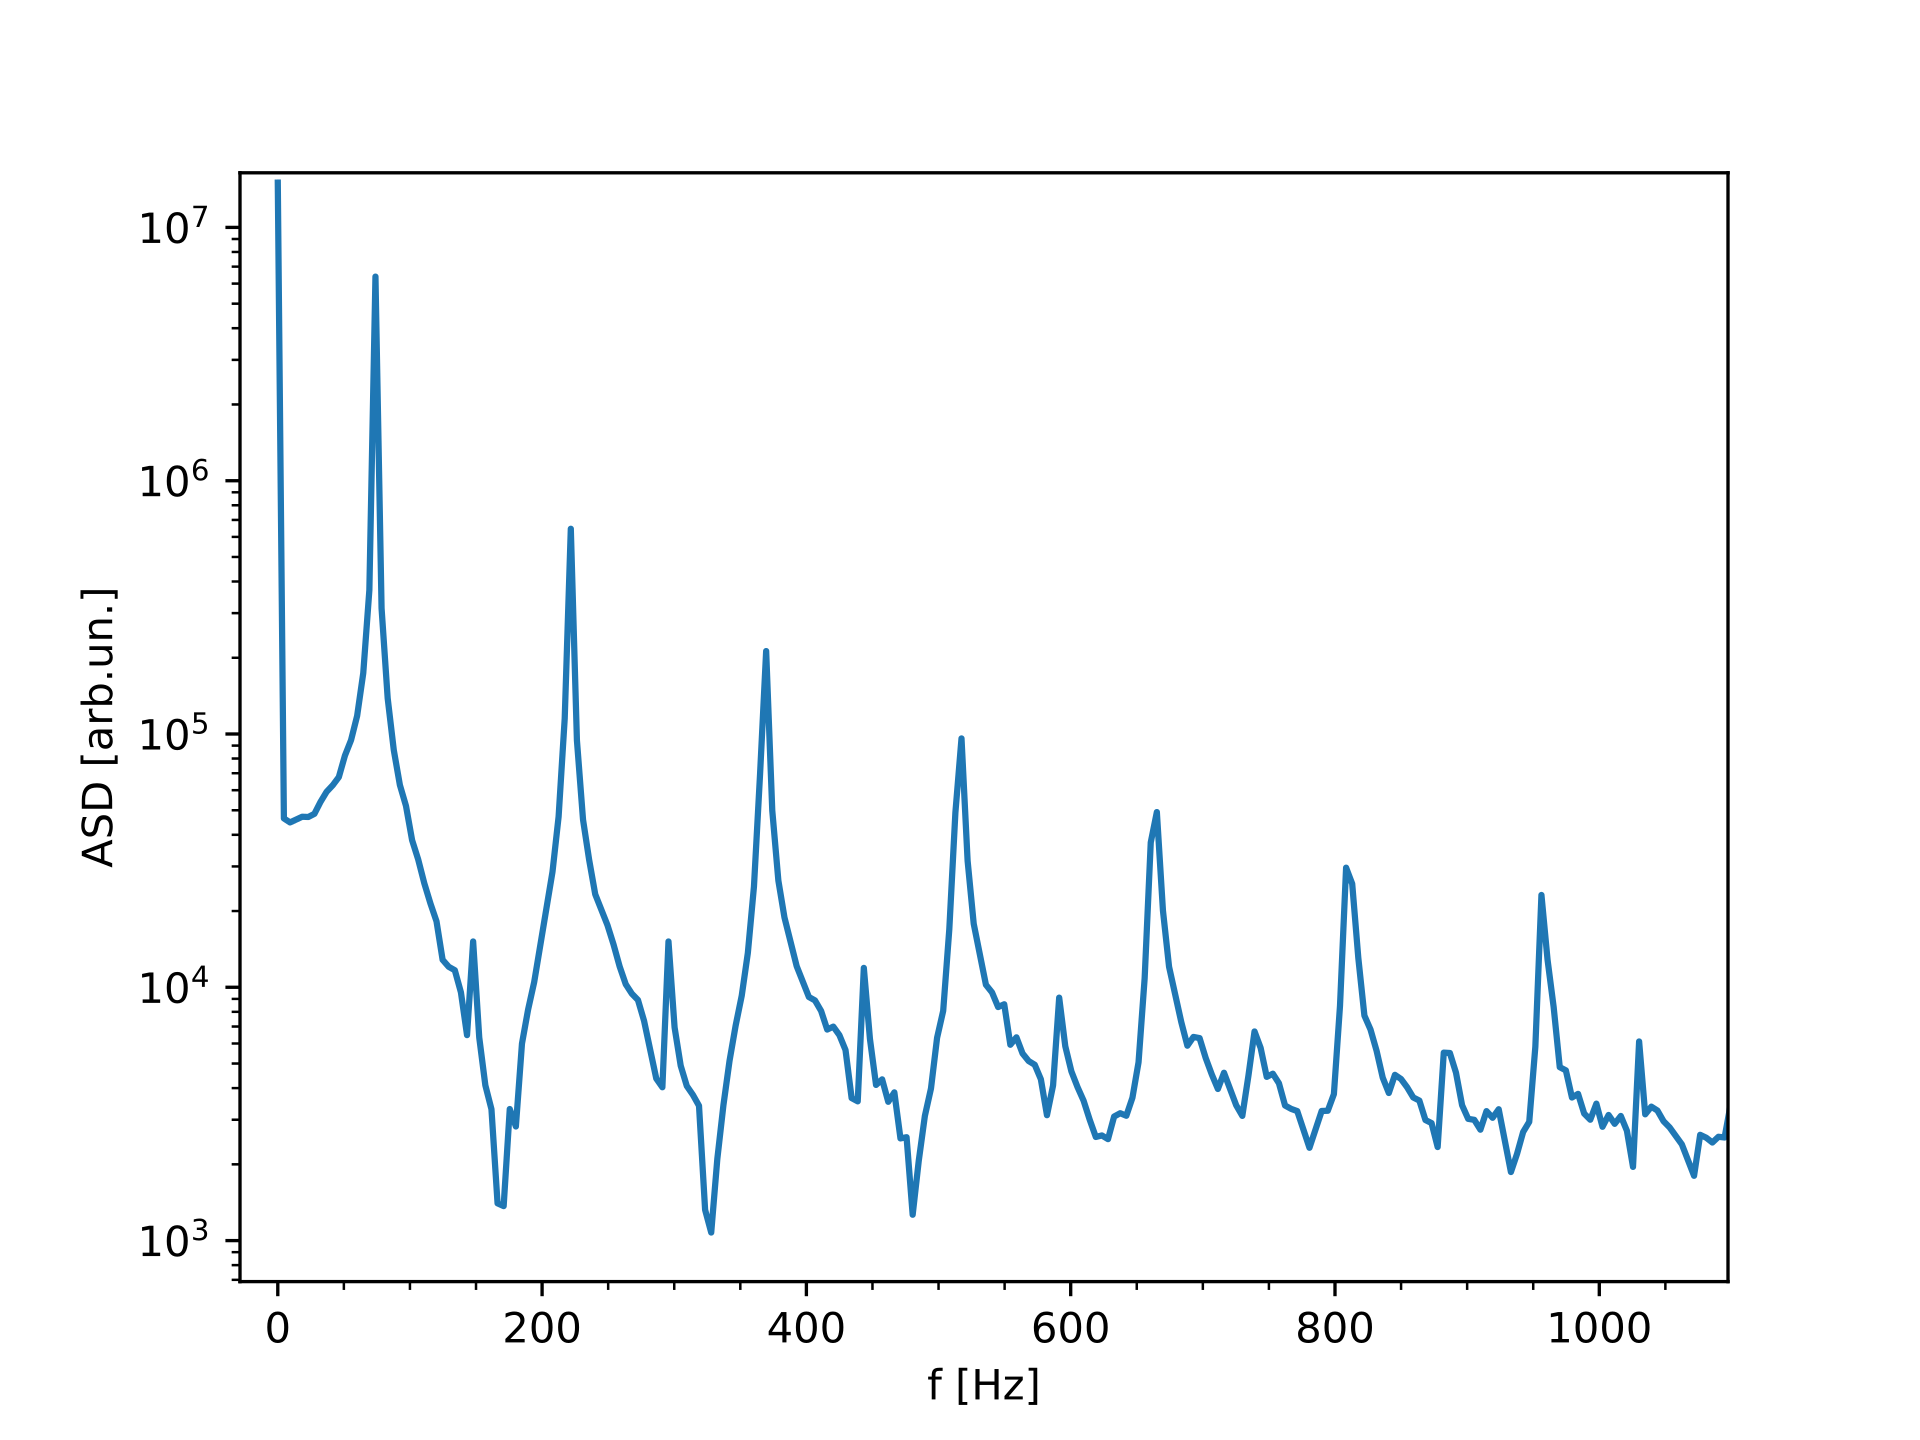
\includegraphics[width=0.48\columnwidth]{img/ese5/f73_TN-tagl}
    \caption{Grafici relativi ad un'onda triangolare a frequenza (72.918 $\pm$ 0.001) Hz. Notare i picchi in corrispondenza delle armoniche dispari.}
    \label{fig:ese5-f73_TN}
\end{figure}

\begin{figure}[H]
    \centering
    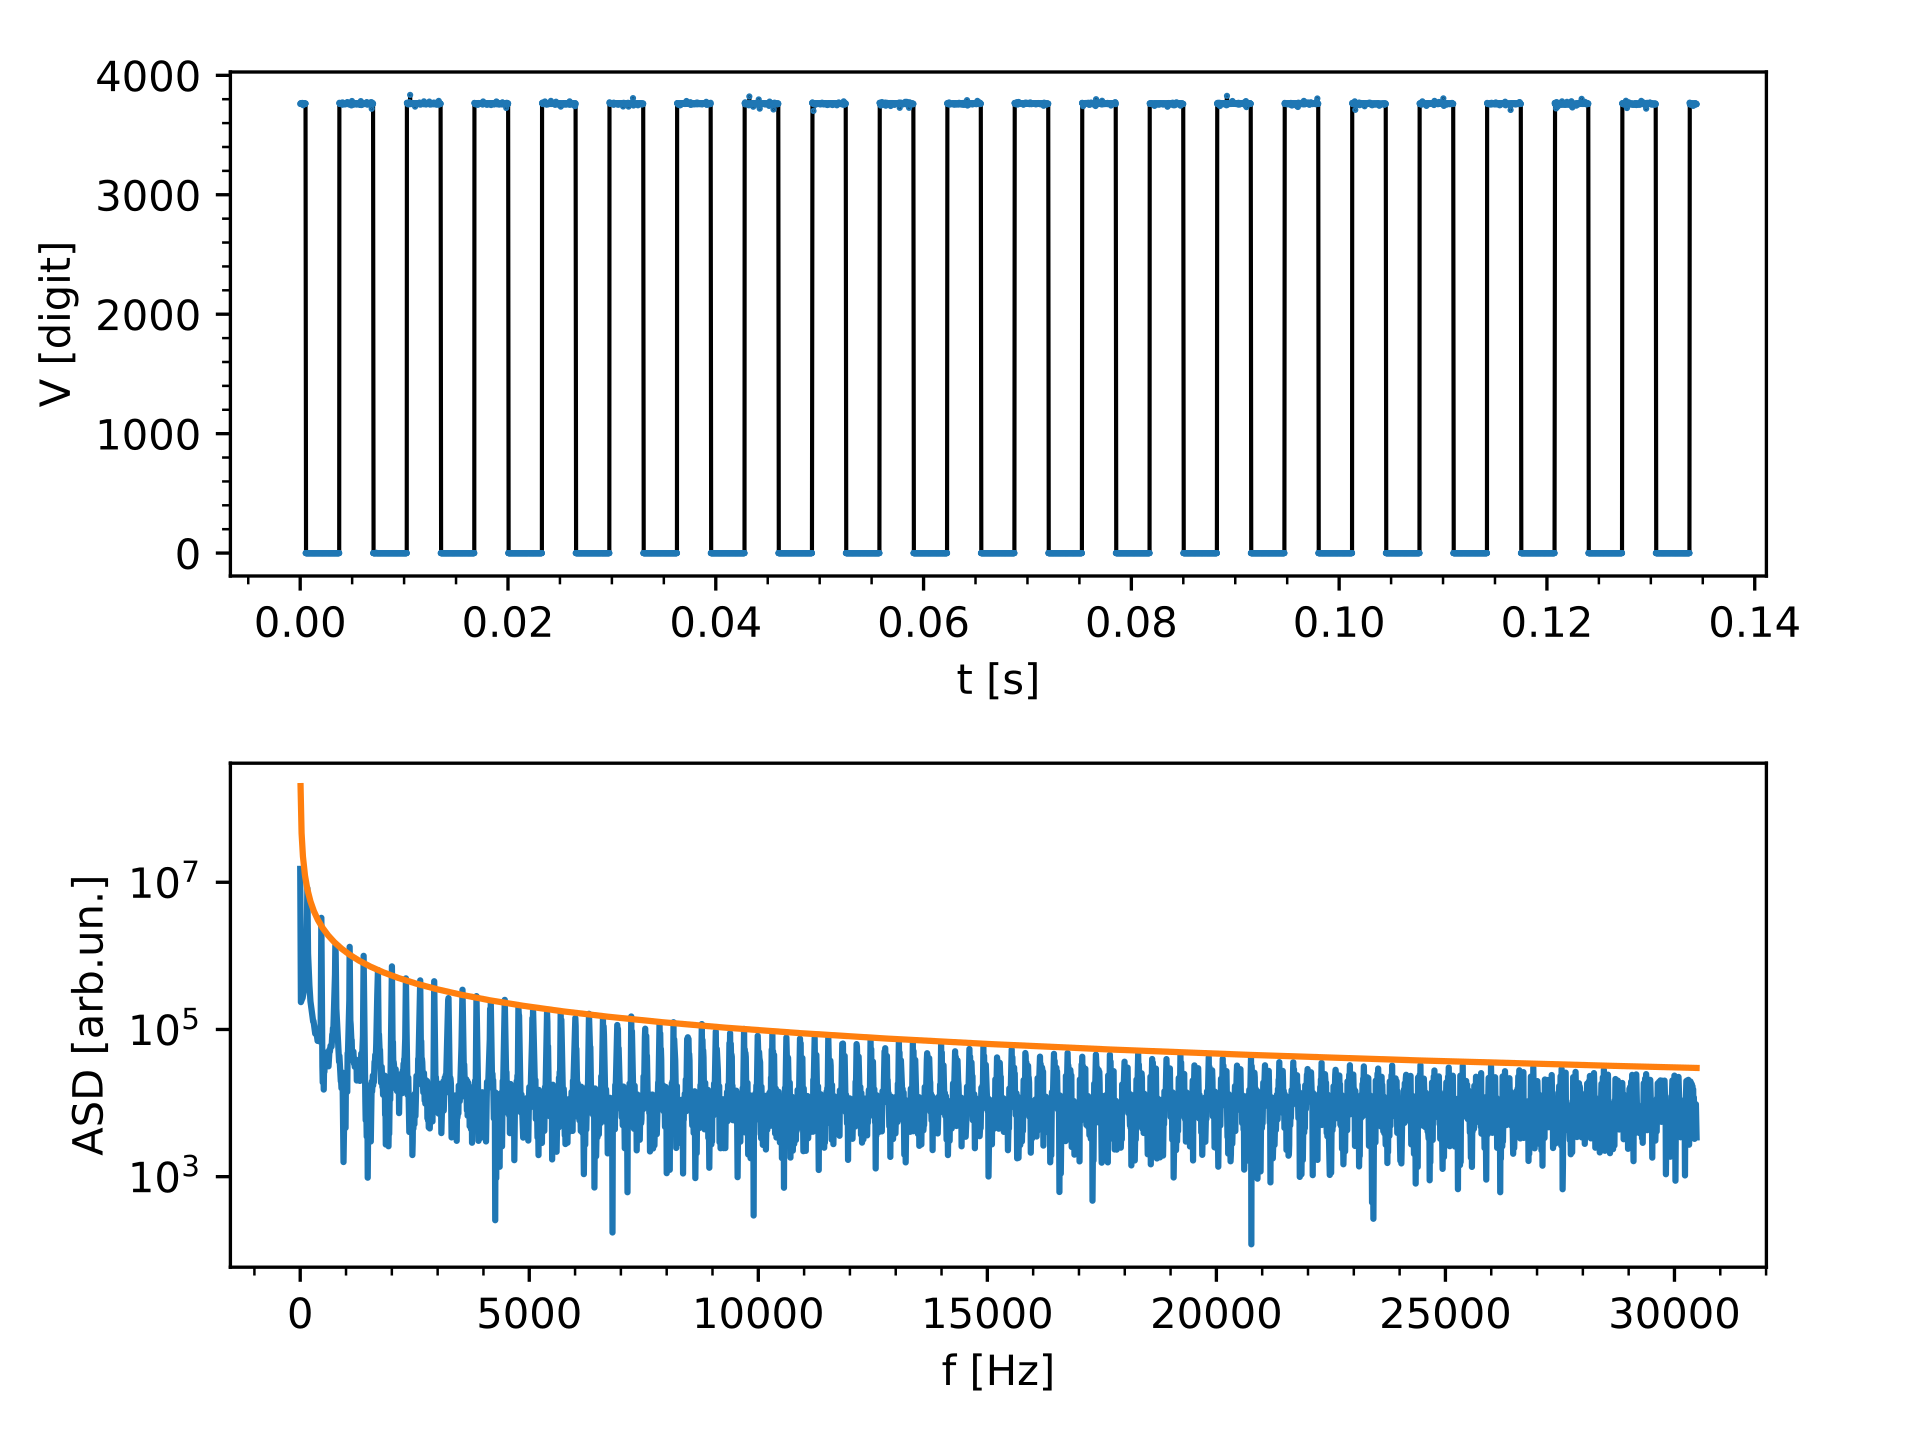
\includegraphics[width=0.45\columnwidth]{img/ese5/f153_QN-retta}
    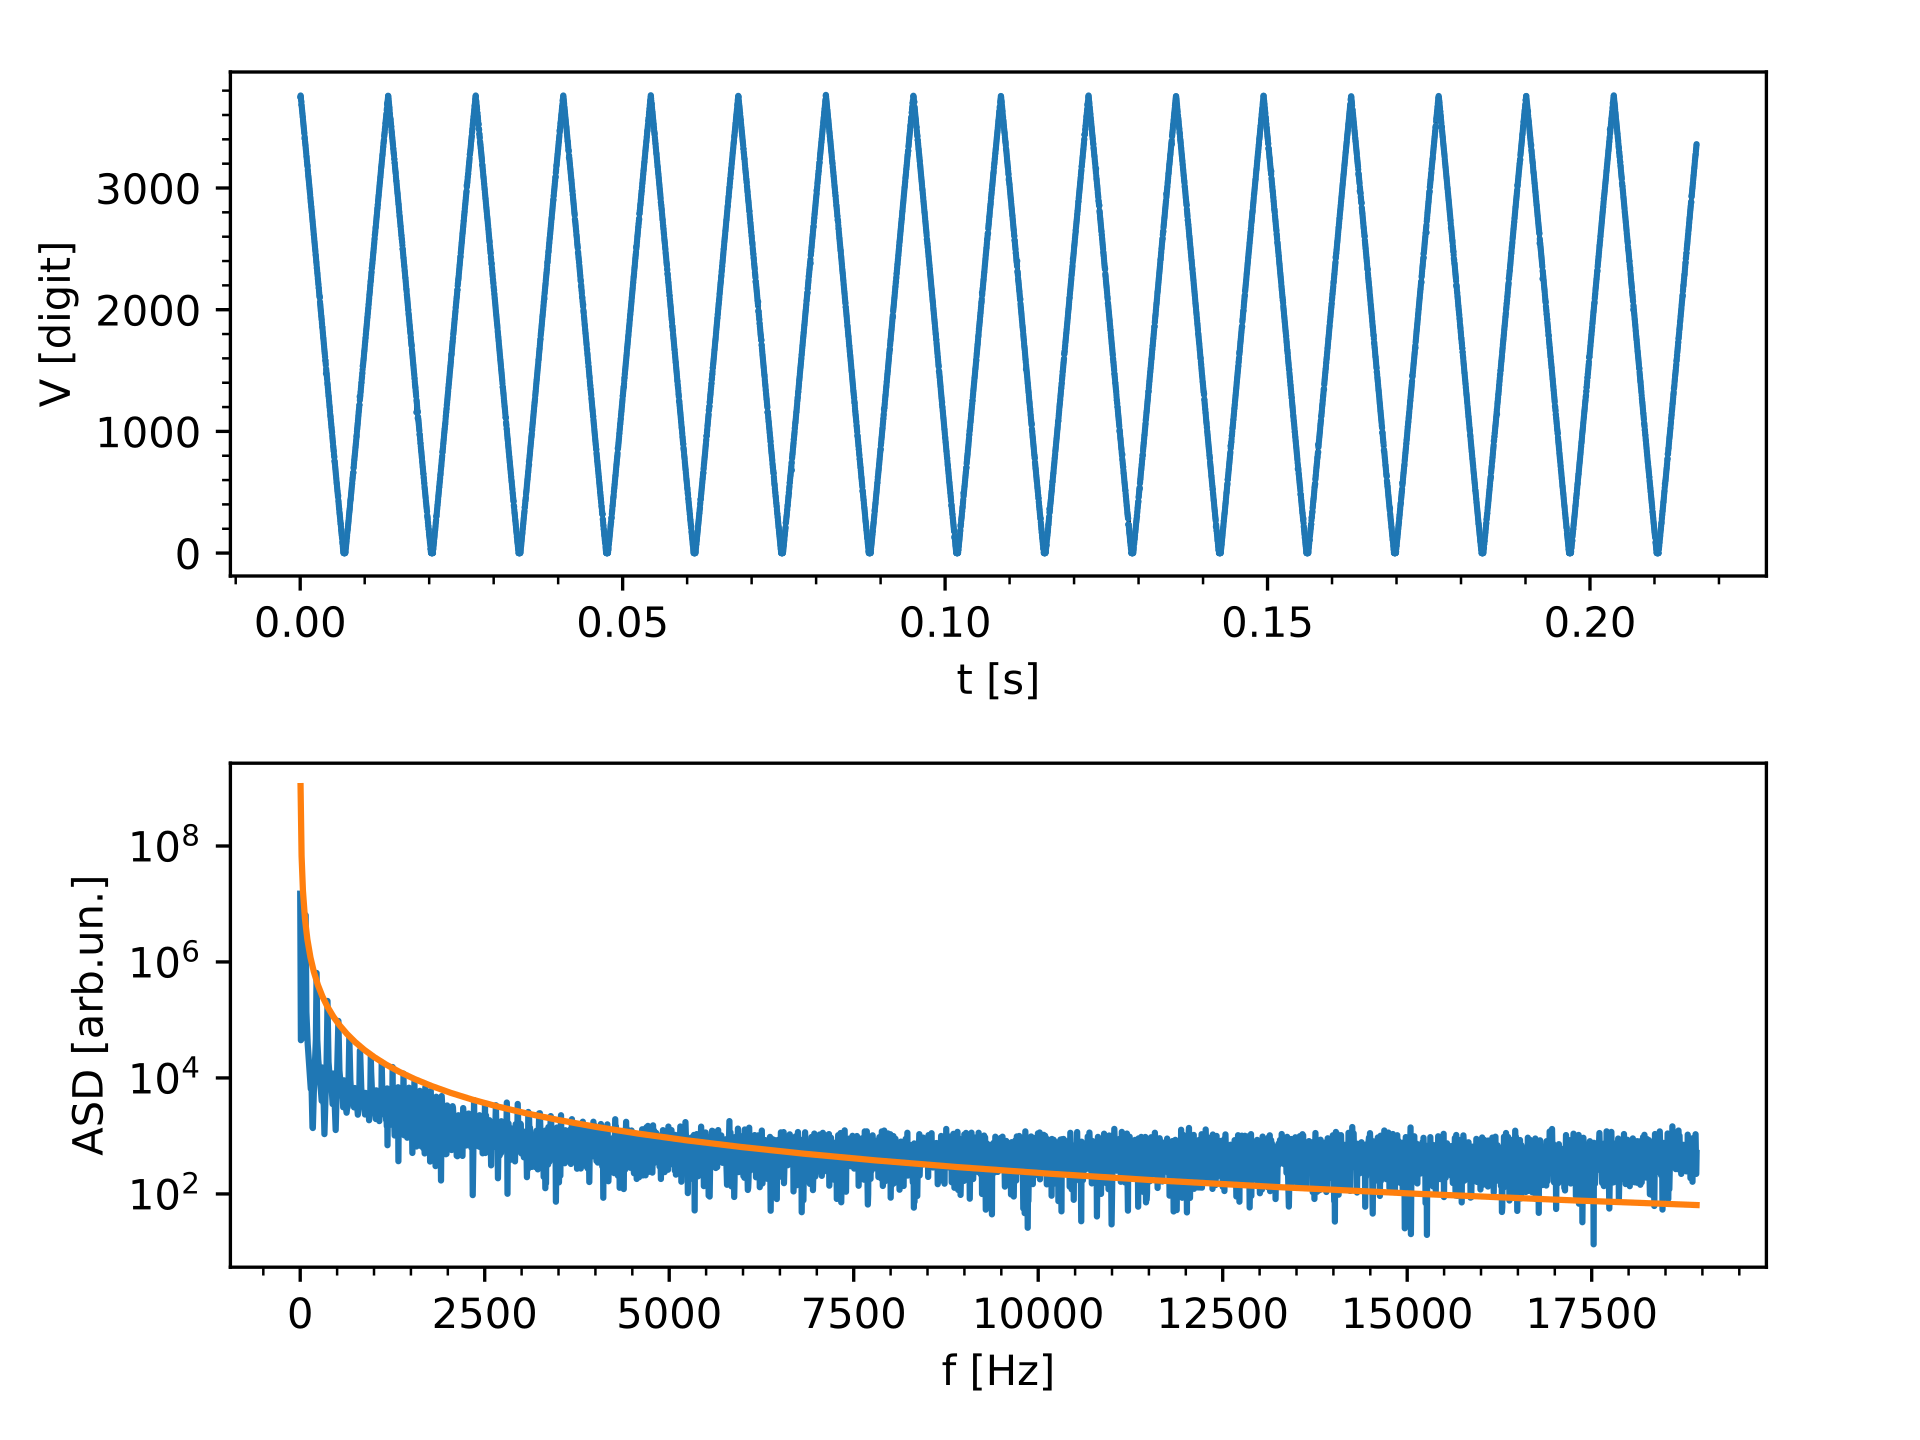
\includegraphics[width=0.45\columnwidth]{img/ese5/f73_TN-retta}
    \caption{Grafici relativi agli stessi dati delle figure \ref{fig:ese5-f73_QN} e \ref{fig:ese5-f73_TN}, con le curve di tendenza dei picchi.}
    \label{fig:ese5-rette}
\end{figure}

\begin{figure}[H]
    \centering
    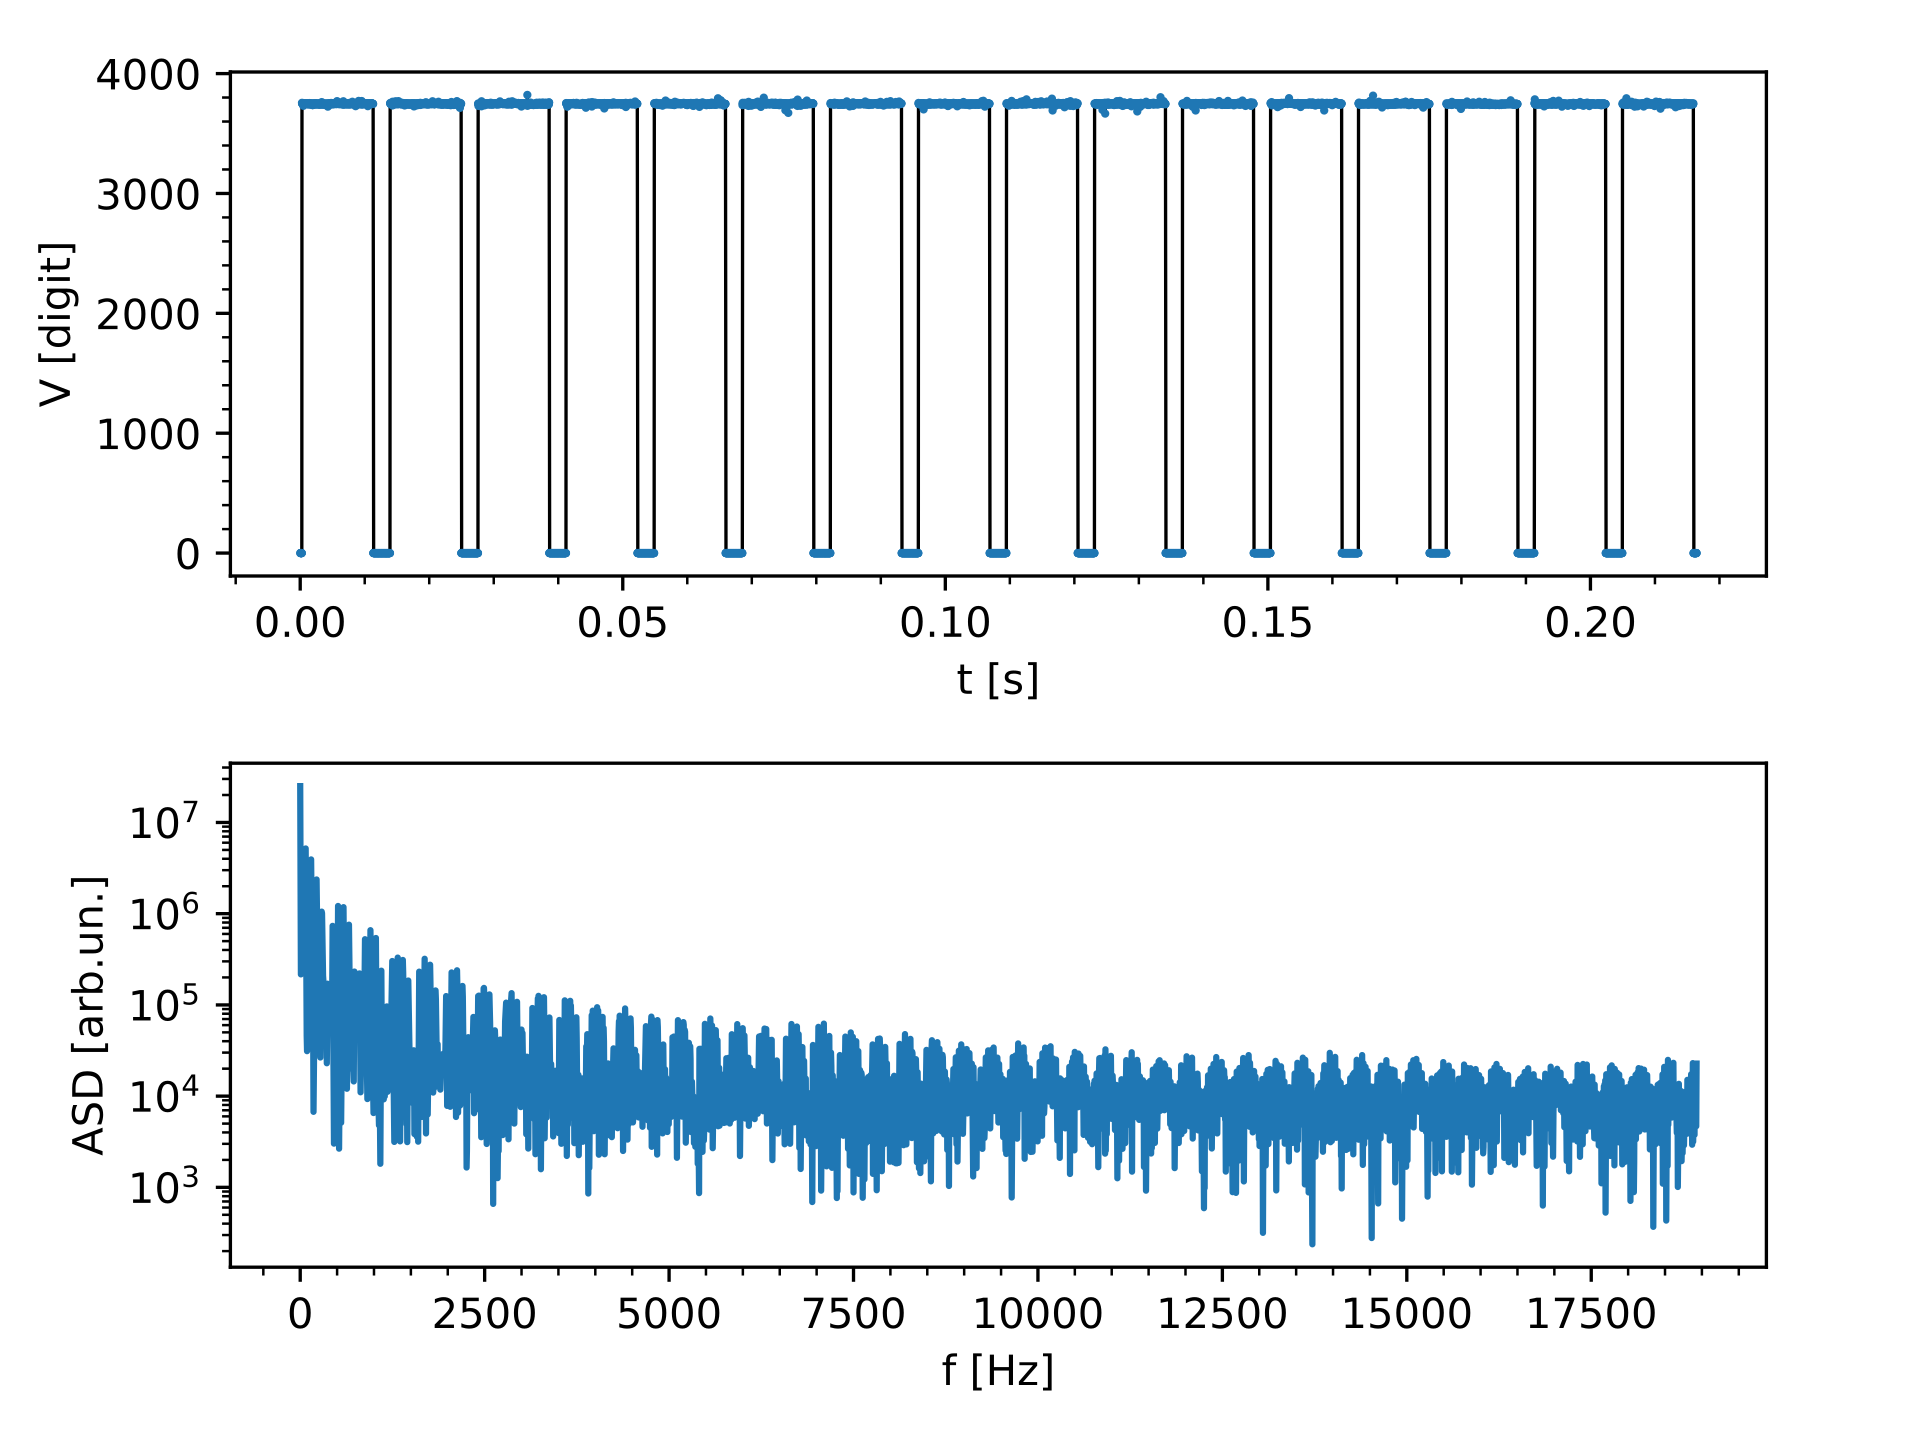
\includegraphics[width=0.45\columnwidth]{img/ese5/f73_QS}
    \includegraphics[width=0.48\columnwidth]{img/ese5/f73_QS-tagl}
    \caption{Grafici relativi ad un'onda quadra a frequenza (73.483 $\pm$ 0.001) Hz con manopola del \textit{duty cycle} girata completamente a sinistra.}
    \label{fig:ese5-duty-sx}
\end{figure}

\begin{figure}[H]
    \centering
    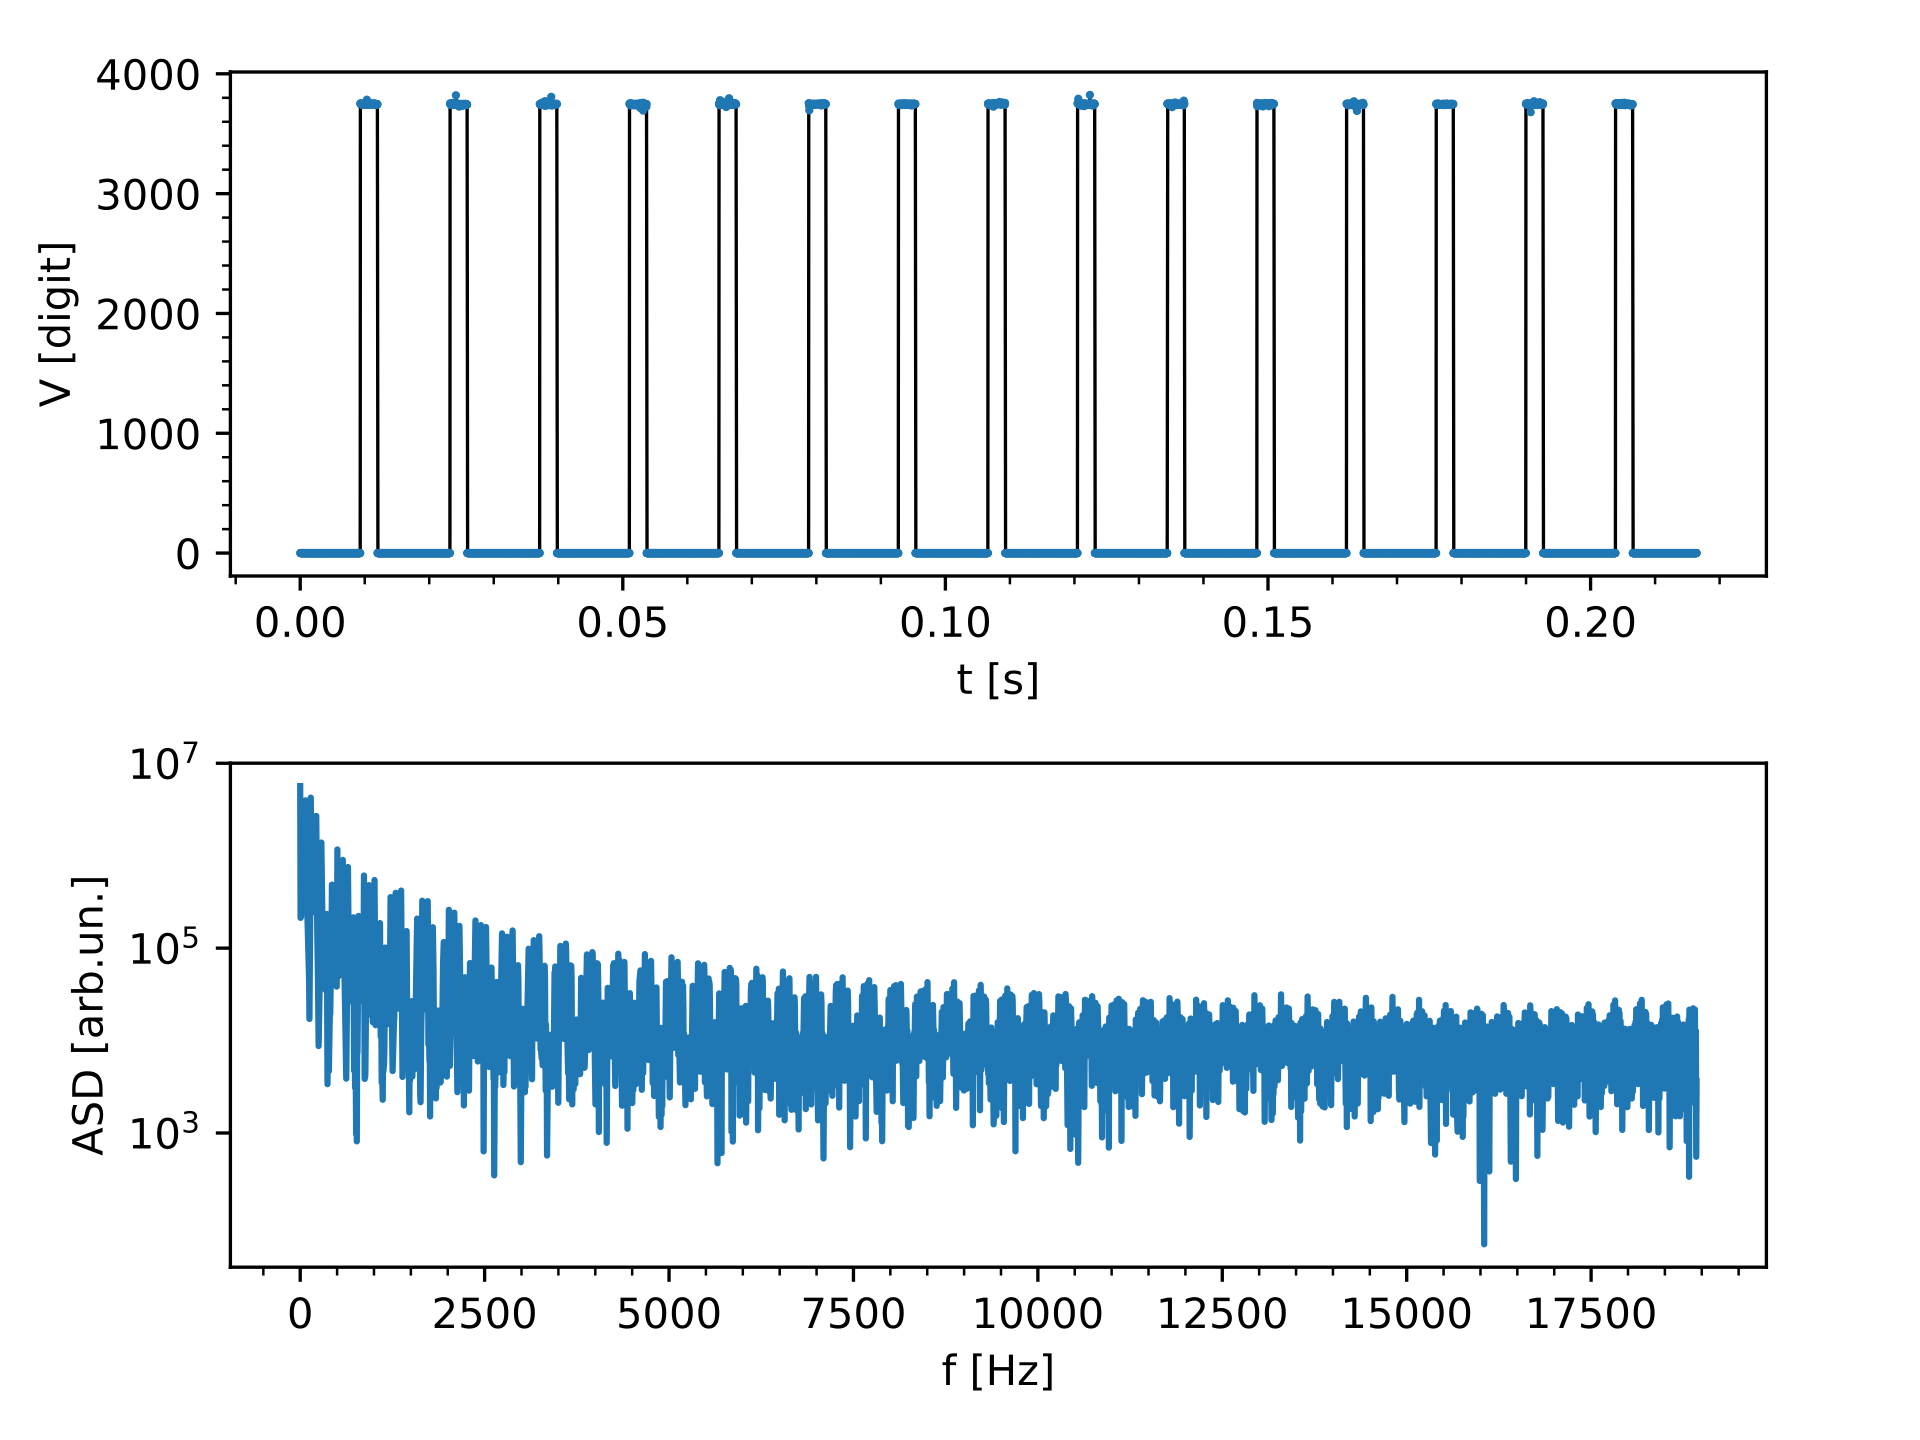
\includegraphics[width=0.45\columnwidth]{img/ese5/f73_QD}
    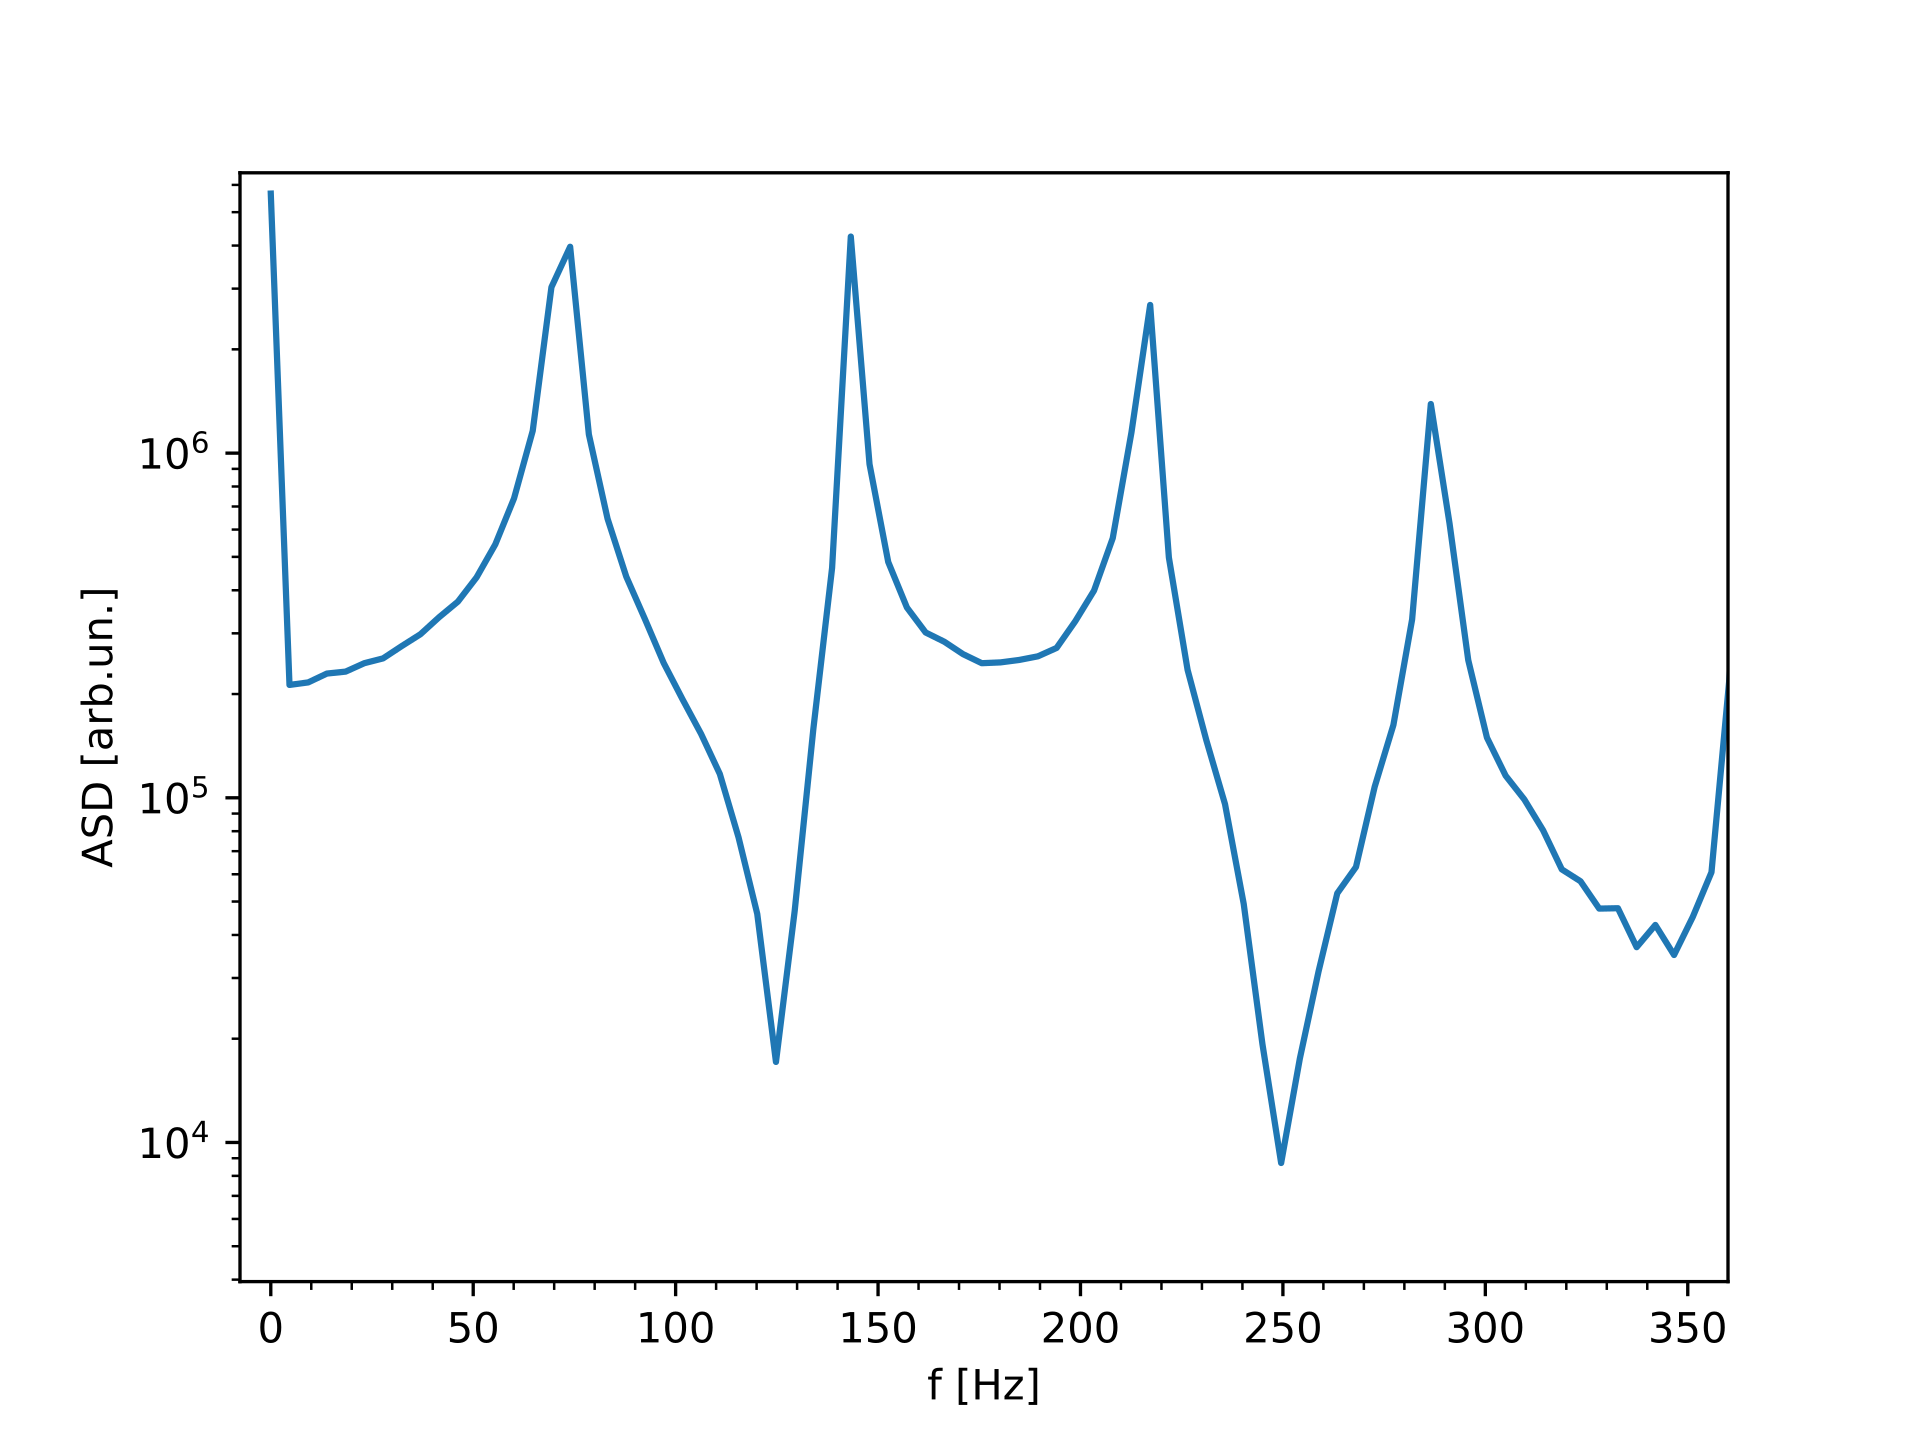
\includegraphics[width=0.48\columnwidth]{img/ese5/f73_QD-tagl}
    \caption{Grafici relativi ad un'onda quadra a frequenza (73.223 $\pm$ 0.001) Hz con manopola del \textit{duty cycle} girata completamente a destra.}
    \label{fig:ese5-duty-dx}
\end{figure}

\section{Pinna di squalo}
I dati graficati in questa sezione sono stati ottenuti facendo passare onde quadre e, in un caso, triangolare attraverso un integratore (con frequenza di taglio $f_T =$482 Hz). Per una maggiore leggibilità, abbiamo preferito riportare solamente il grafico della FFT zoomato sull'intorno del picco di nostro interesse.\\
Notiamo che i picchi delle armoniche seguono un andamento maggiormente decrescente rispetto a quanto osservato nella sezione precedente. Questo è dovuto al fatto che l'integratore funge da filtro passa basso. Per uno dei set di dati (a frequenza (501.00 $\pm$ 0.01) Hz) abbiamo rappresentato la curva corrispondente ad una legge di potenza moltiplicata per il guadagno dell'integratore. Abbiamo notato che anche in questo caso, come per la sezione precedente, i picchi dell'onda di partenza seguivano un andamento del tipo $n^{-1.06}$, invece che $n^{-1}$ come atteso per un'onda quadra ideale.

\begin{figure}[H]
    \centering
    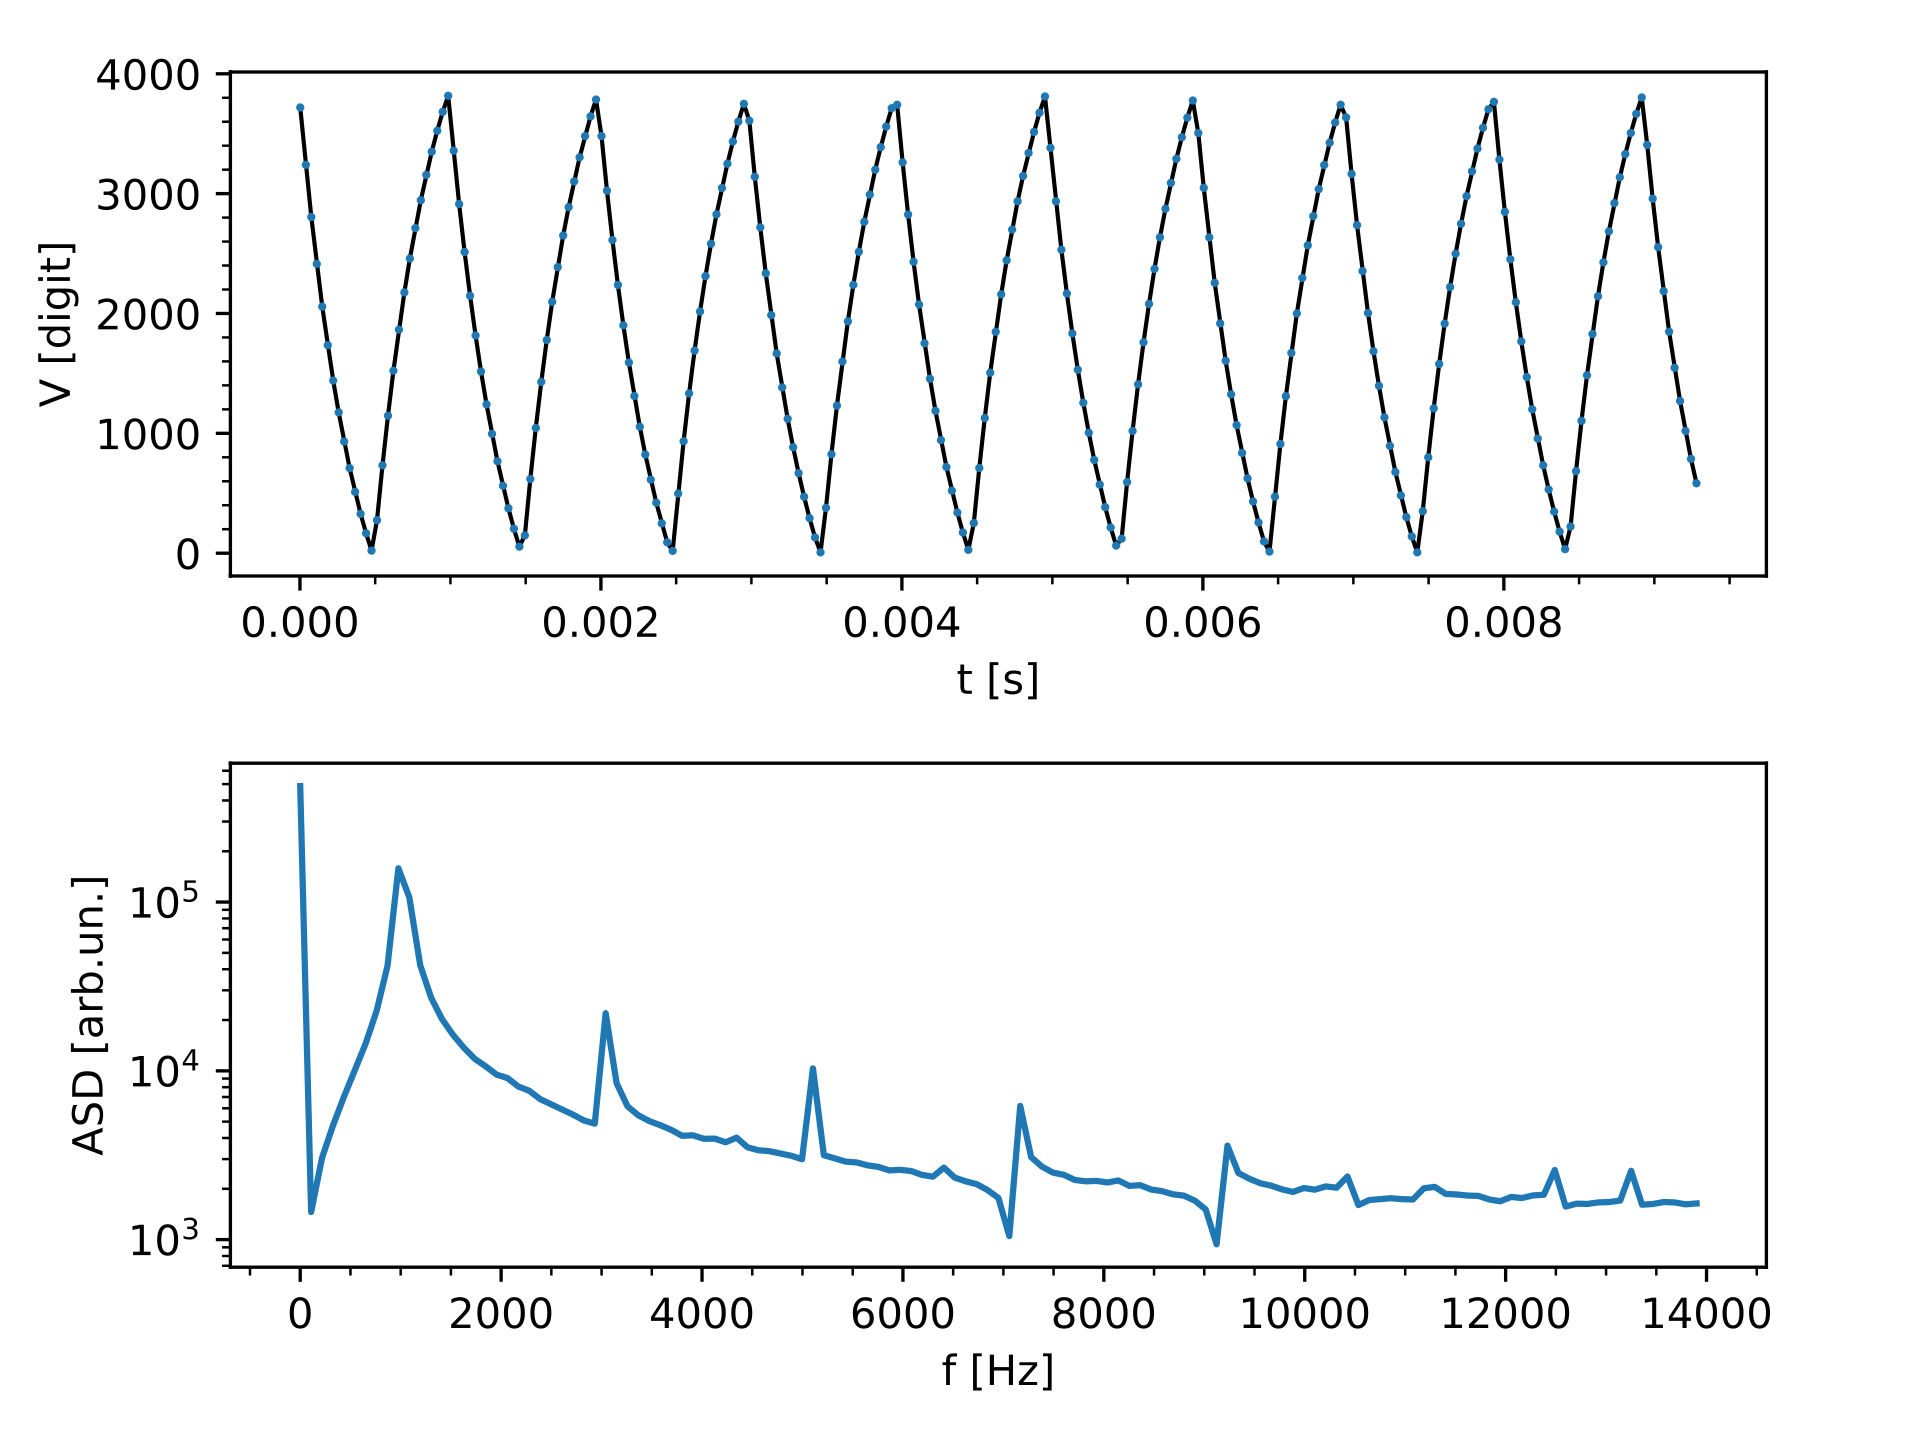
\includegraphics[width=0.48\columnwidth]{img/ese6/esp6-1.0082kHz.png}
    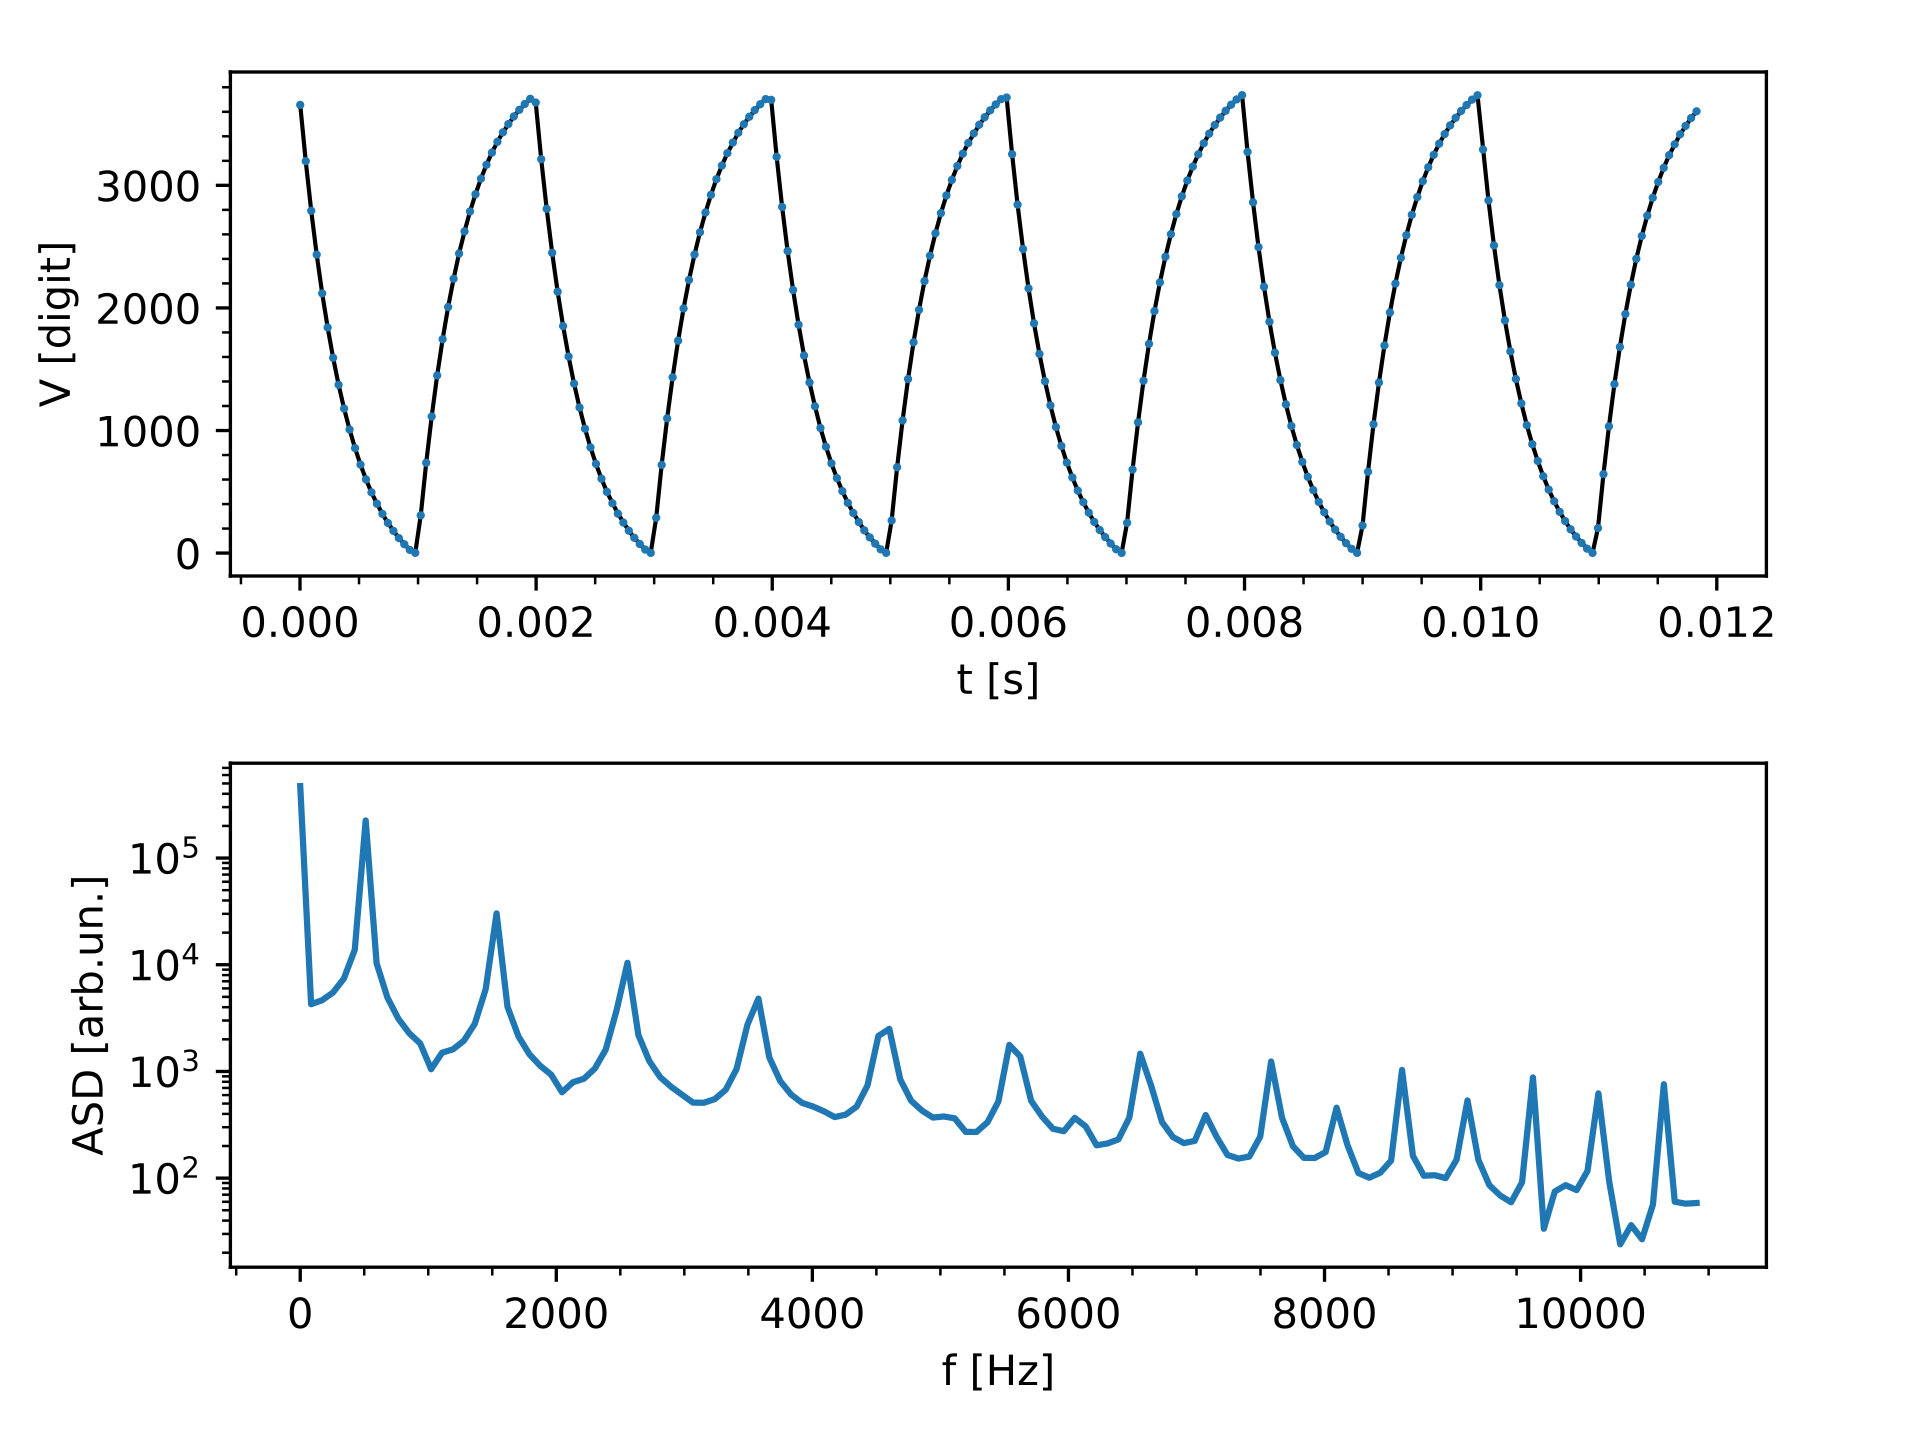
\includegraphics[width=0.48\columnwidth]{img/ese6/esp6-501.00Hz.png}
    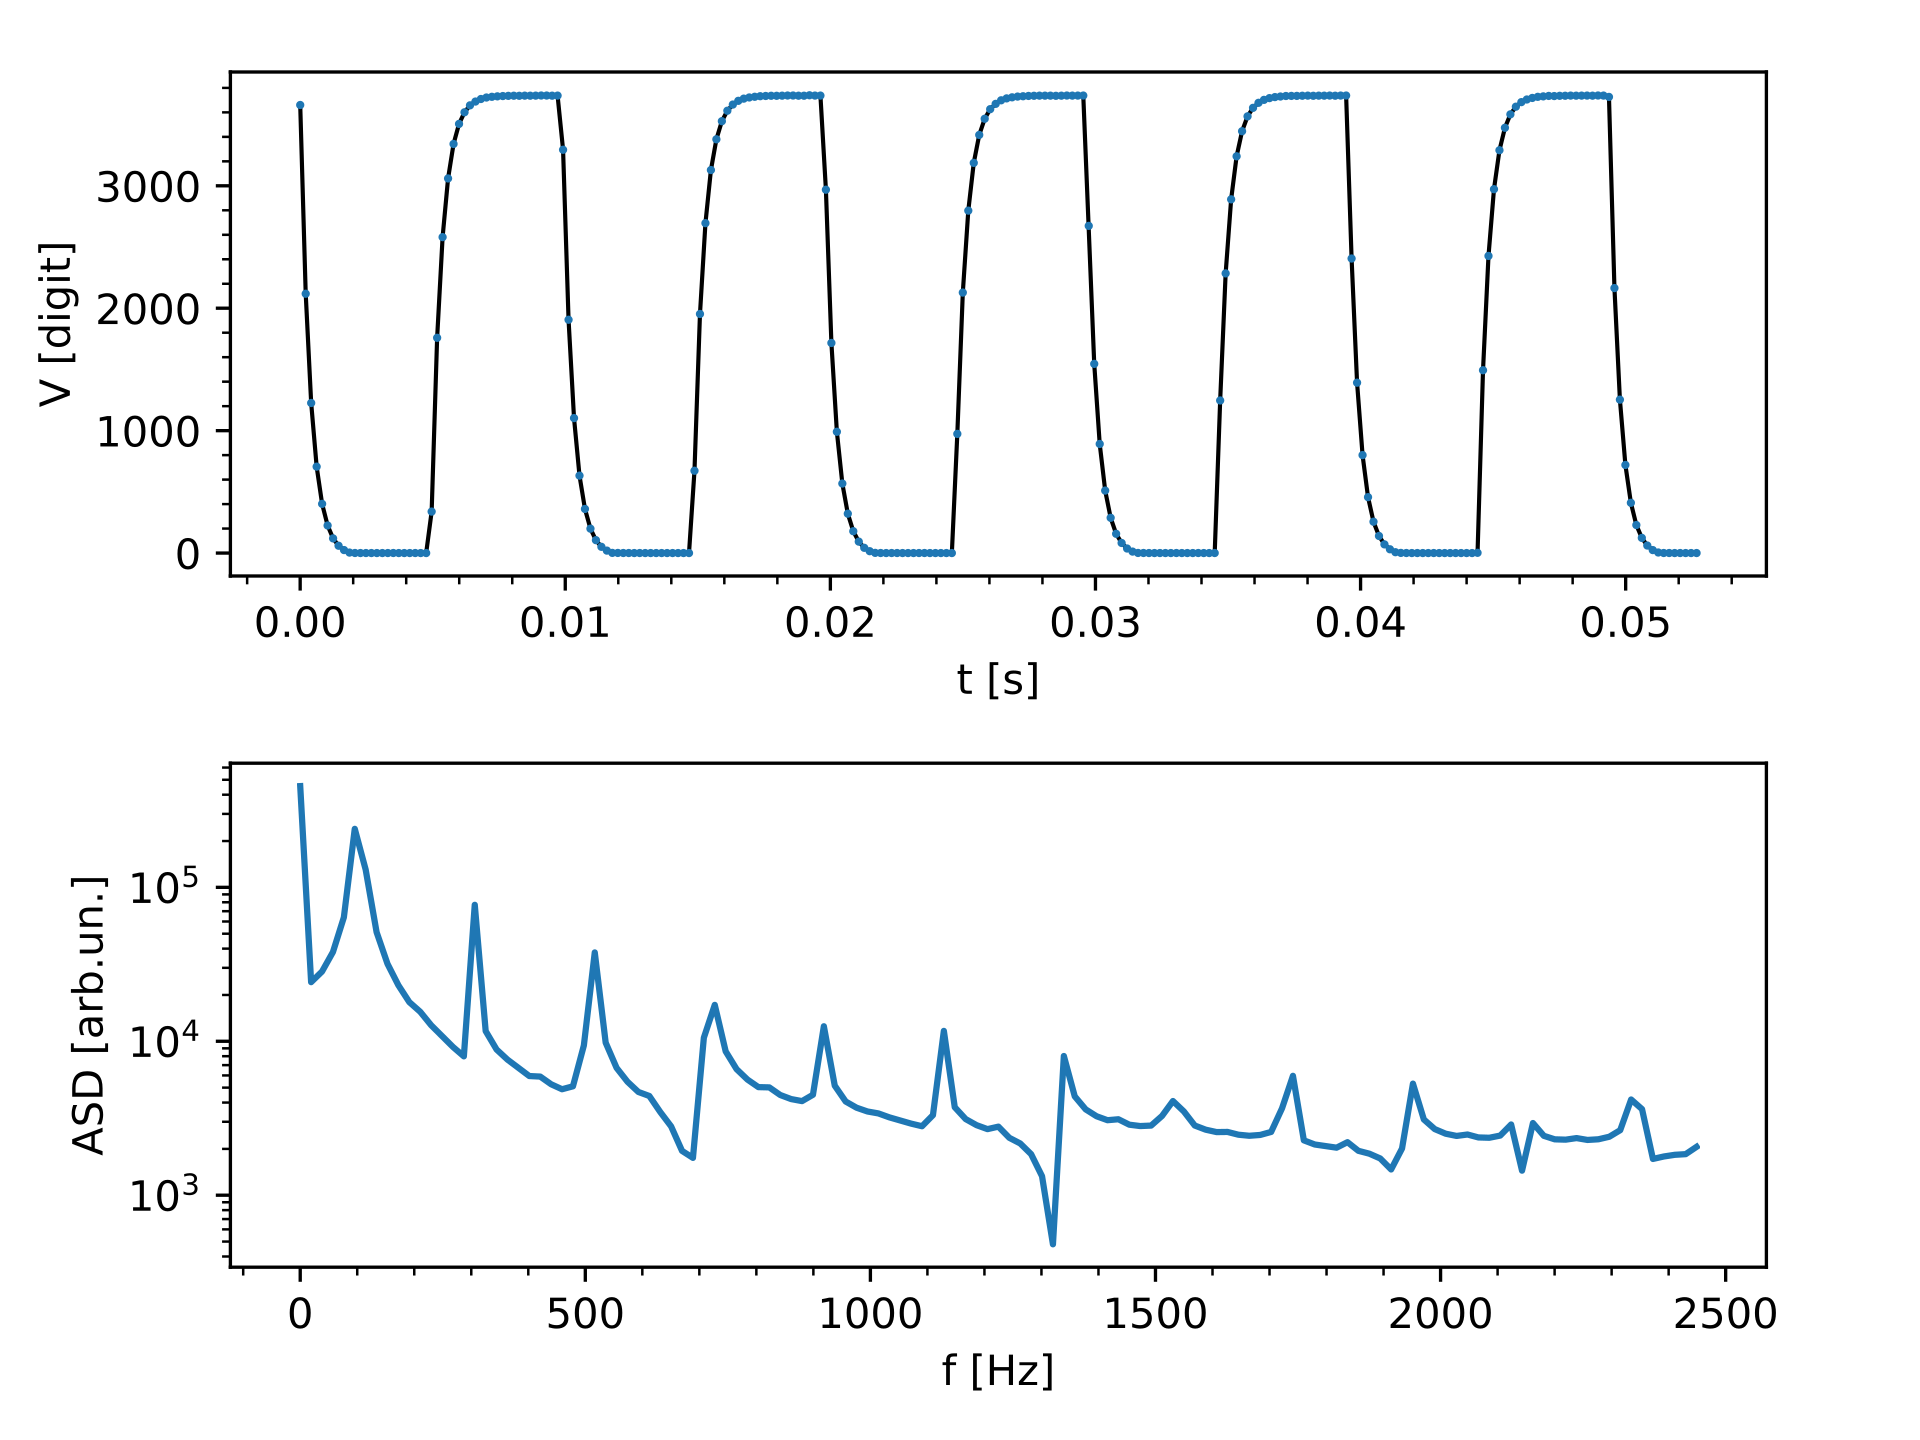
\includegraphics[width=0.48\columnwidth]{img/ese6/esp6-101.26Hz.png}
    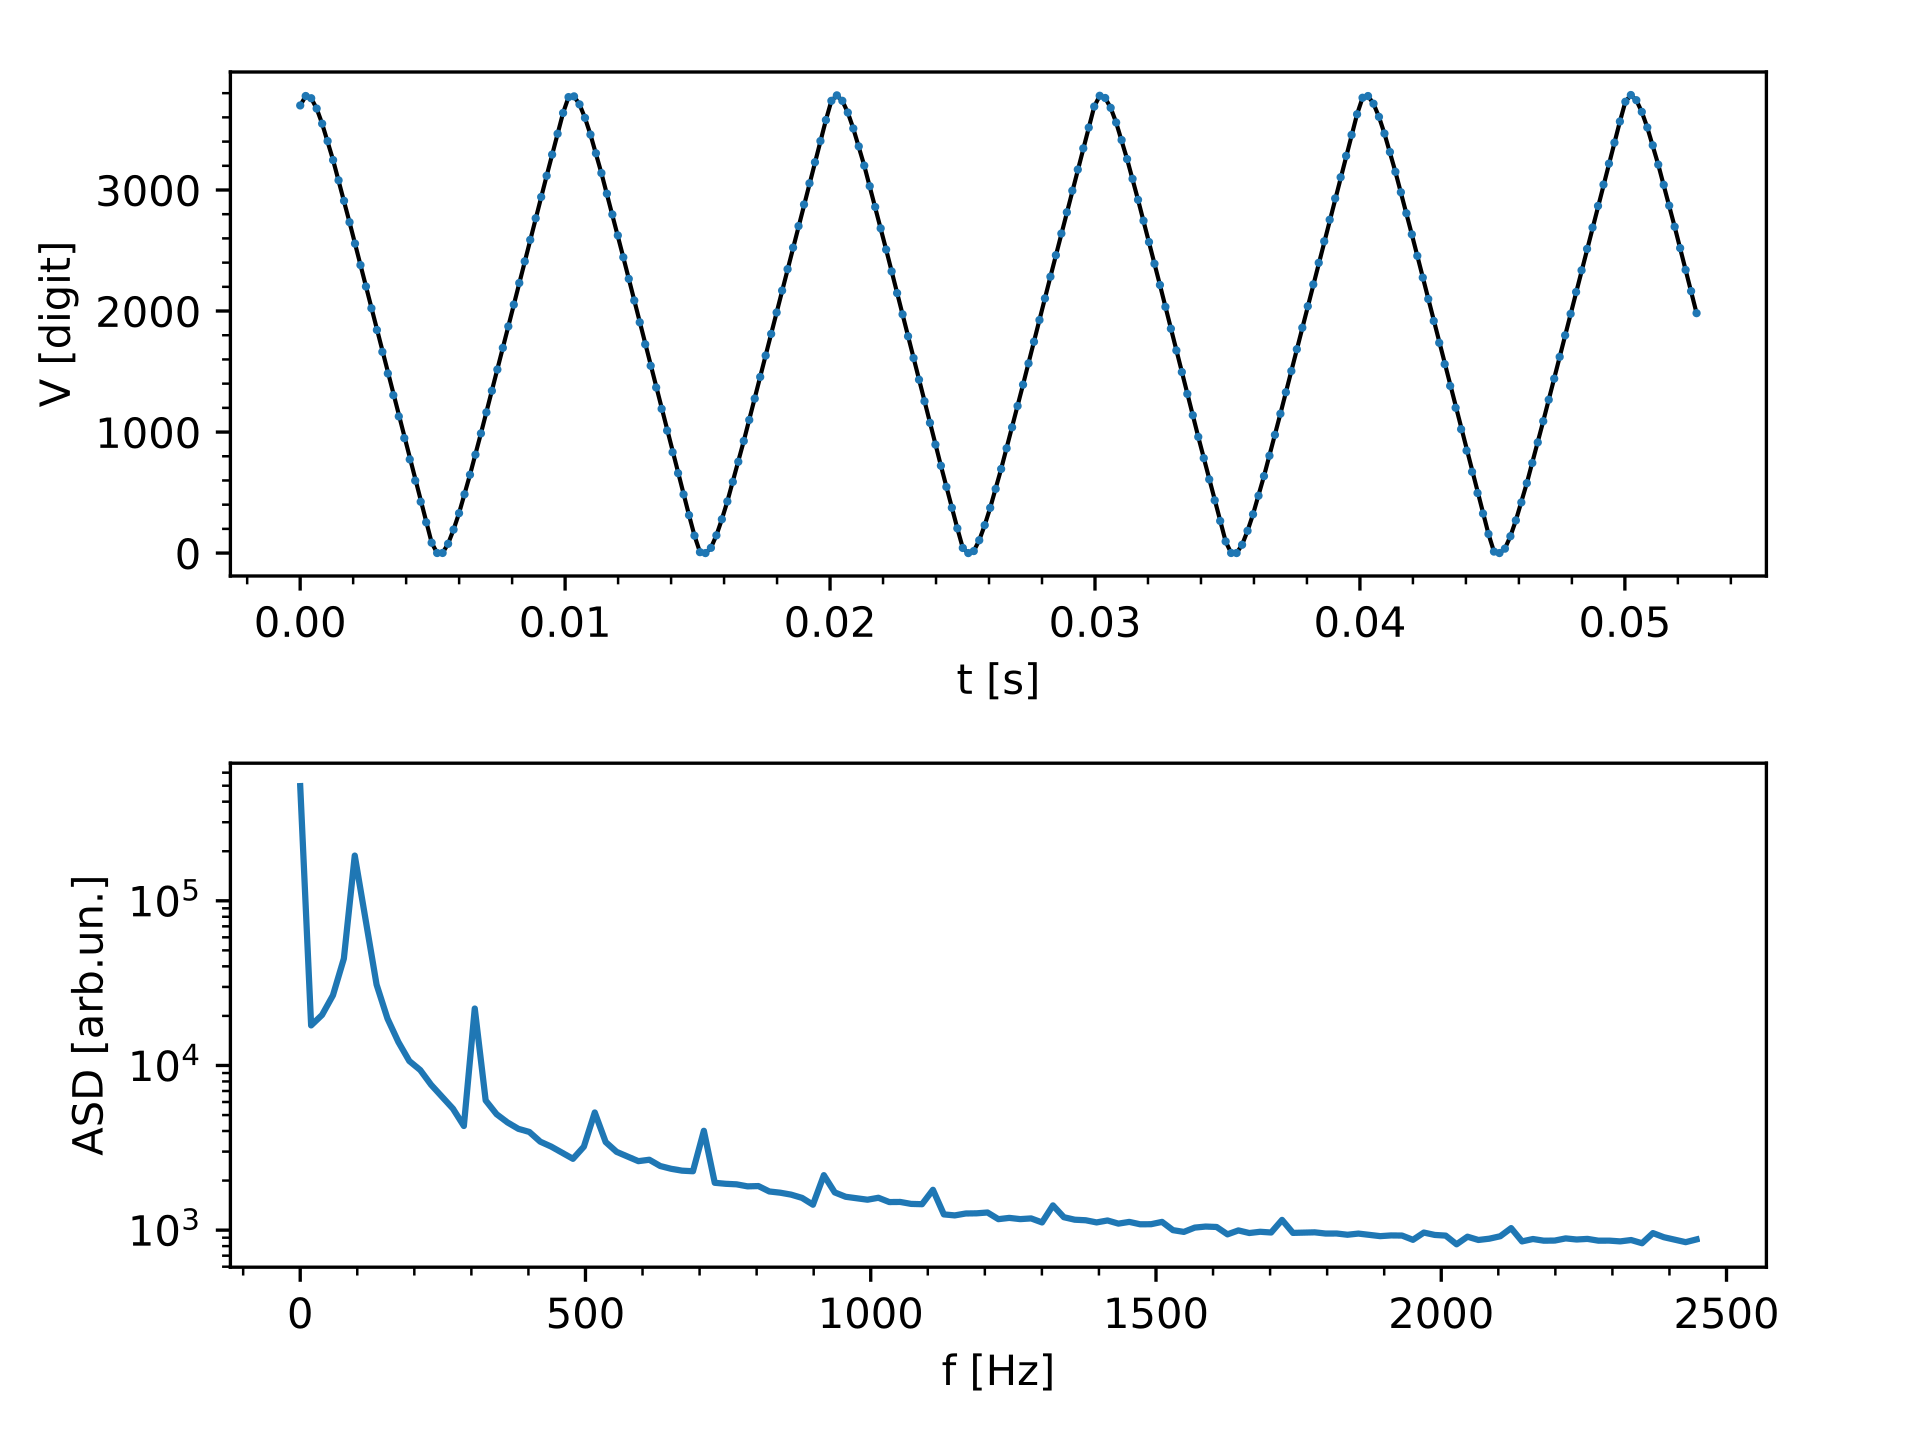
\includegraphics[width=0.48\columnwidth]{img/ese6/esp6-100.06Hz-T.png}
    \caption{Da sinistra a destra: Onde quadre rispettivamente a frequenze (1.0082 $\pm$ 0.0001) kHz, (501.00 $\pm$ 0.01) Hz, (101.26 $\pm$ 0.01) Hz; Onda triangolare a frequenza (100.06 $\pm$ 0.01) Hz).}
    \label{fig:ese6-grafici}
\end{figure}

\begin{figure}[H]
    \centering
    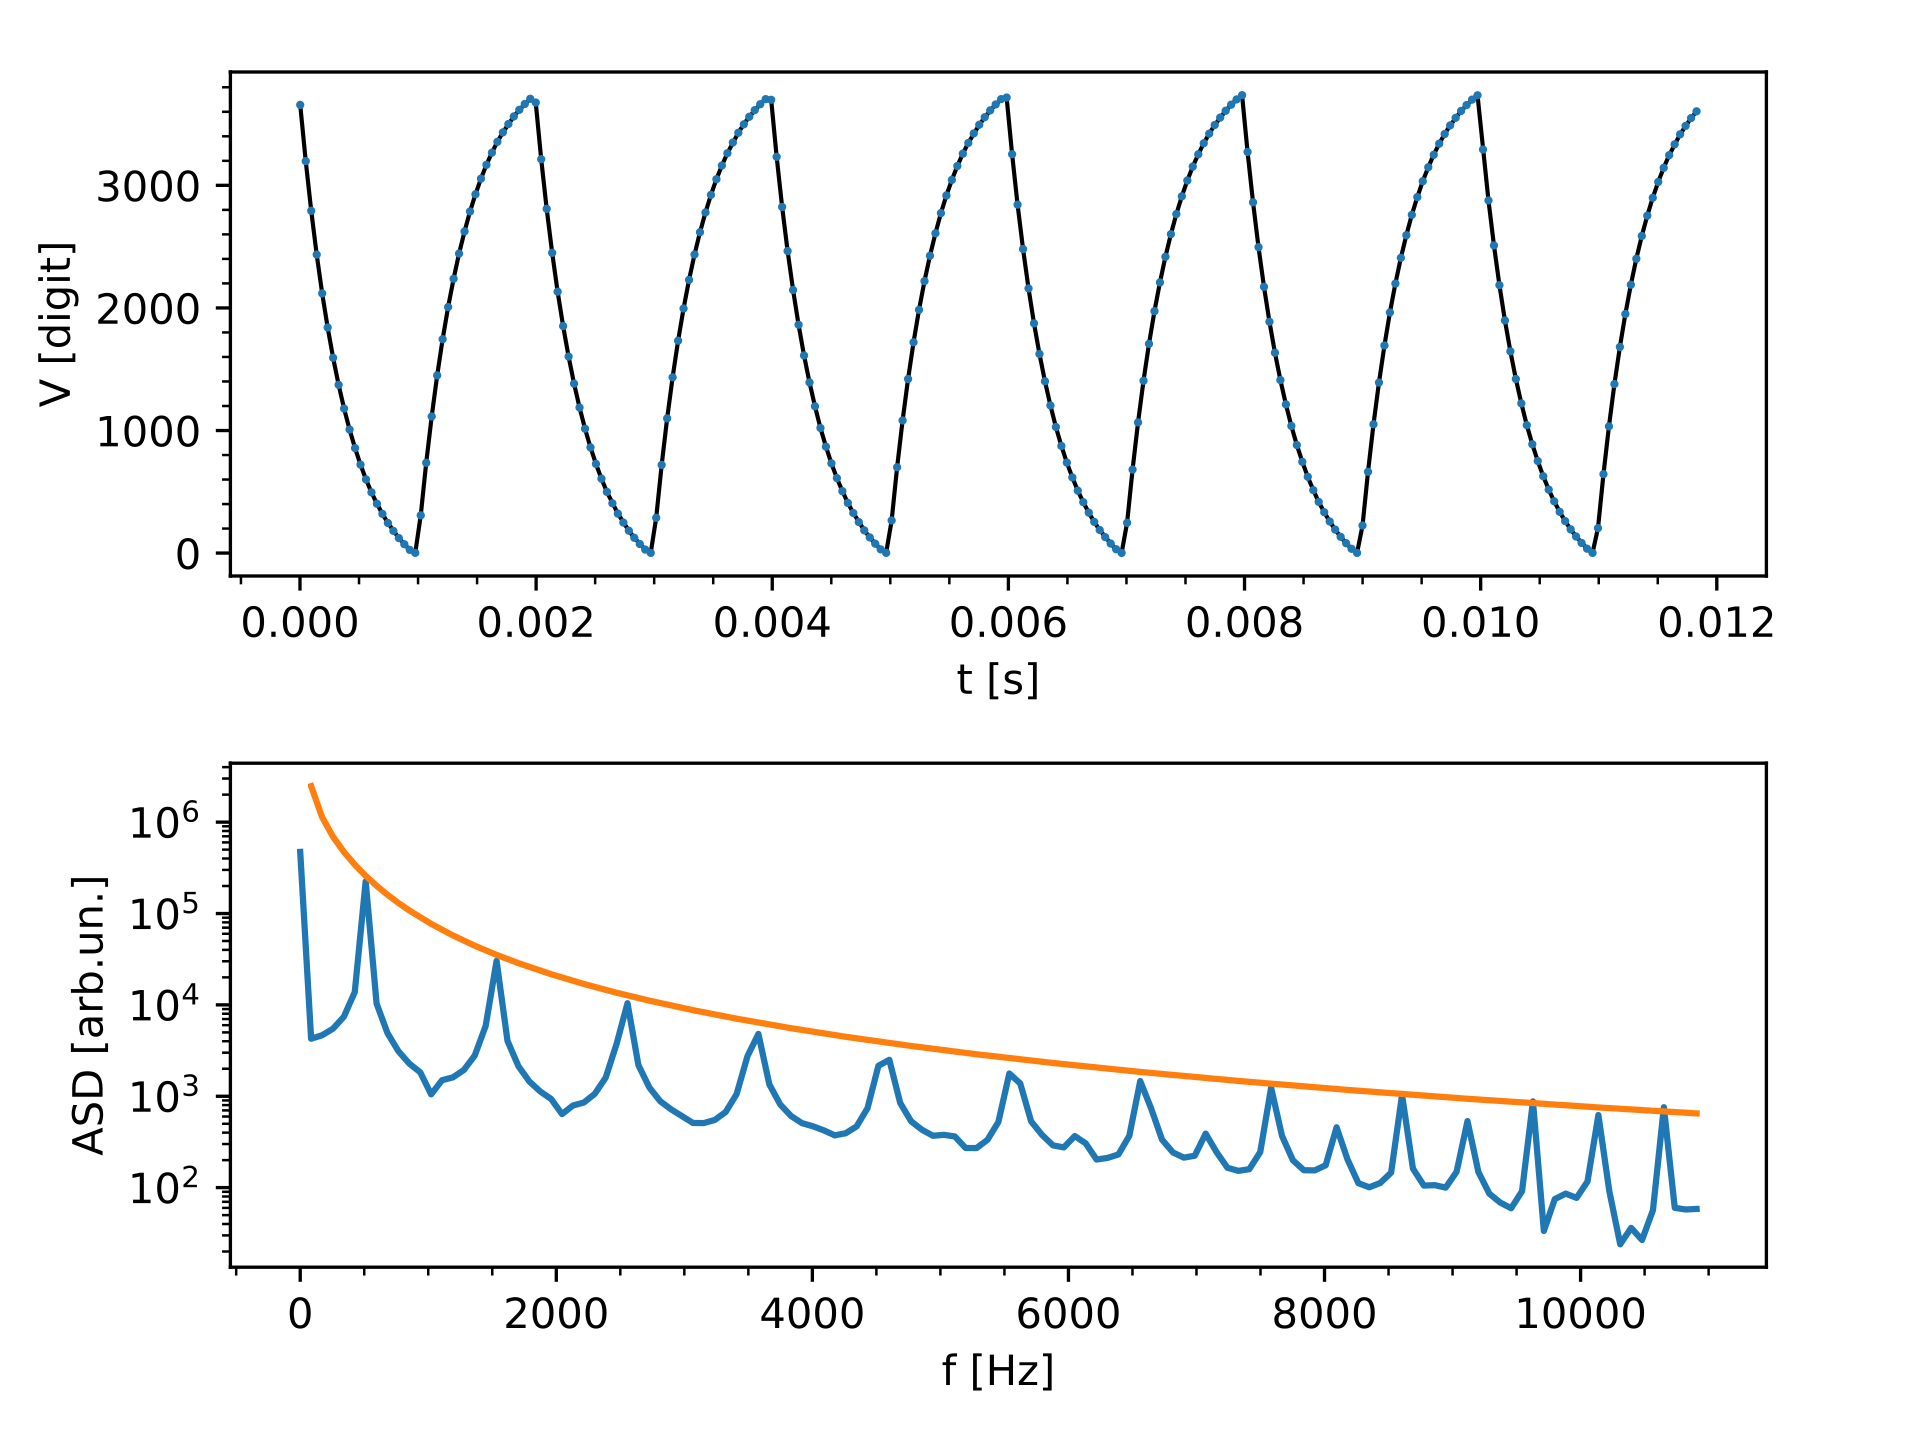
\includegraphics[width=0.80\columnwidth]{img/ese6/esp6-501.00Hz-retta.png}
    \caption{Onda quadra a frequenza (501.00 $\pm$ 0.01) Hz con curva di tendenza dei picchi.}
    \label{fig:ese6-retta}
\end{figure}

\section{Simulazione onda quadra rumorosa}
Nelle due sezioni precedenti, abbiamo notato che le armoniche delle onde quadre seguono un andamento del tipo $n^{-1.06}$. Abbiamo supposto che ciò potesse essere dovuto al rumore prodotto dal generatore. Per verificare tale ipotesi, abbiamo generato un'onda quadra con del rumore gaussiano, con deviazione standard pari a un decimo dell'ampiezza dell'onda.\\
Dal grafico della FFT, abbiamo notato che la nostra assunzione è ragionevole.
\begin{figure}[H]
    \centering
    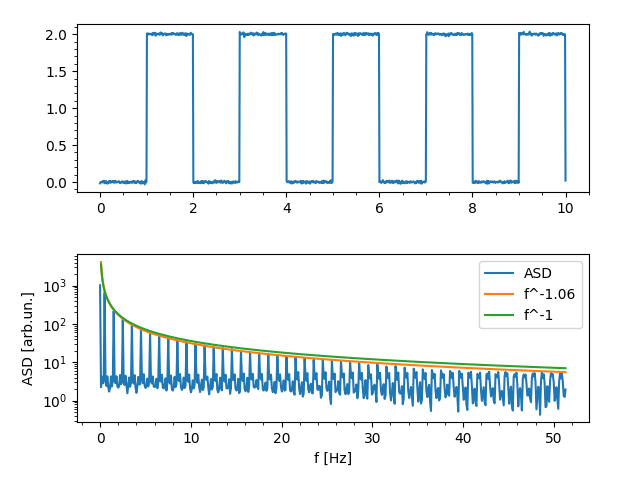
\includegraphics[width=0.80\columnwidth]{img/onda_quadra_noisy.png}
    \caption{Simulazione di un'onda quadra con rumore gaussiano. In verde, l'andamento di un'onda quadra ideale; in arancione, l'andamento da noi osservato sperimentalmente.}
    \label{fig:ese6-retta}
\end{figure}

\section{Resistenza dinamica del diodo e lock-in numerico}
In questa esperienza abbiamo fatto passare un segnale alternato attraverso un diodo polarizzato e misurato la d.d.p. ai capi del diodo. Poiché il segnale alternato veniva fatto passare attraverso prima una resistenza $R_D$ e poi attraverso il diodo, di resistenza dinamica $r_d \ll R_D$, il segnale acquisito finisce per essere molto rumoroso. Ciò nonostante, come è evidente dalla figura \ref{fig:ese9-vd}, nella trasformata di Fourier è presente un picco alla stessa frequenza di quello presente nella figura \ref{fig:ese9-VG} (1.03 kHz), per cui il segnale è comunque identificabile nei dati acquisiti.\\
Nella figura \ref{fig:ese9-lockin}, usando il valore della trasformata di Fourier in corrispondenza del picco della figura \ref{fig:ese9-vd}, abbiamo ricostruito il segnale. I grafici mostrano i dati acquisiti e l'onda sinusoidale ricostruita, entrambi rappresentati con una linea continua per una maggiore leggibilità. 

\begin{figure}[H]
    \centering
    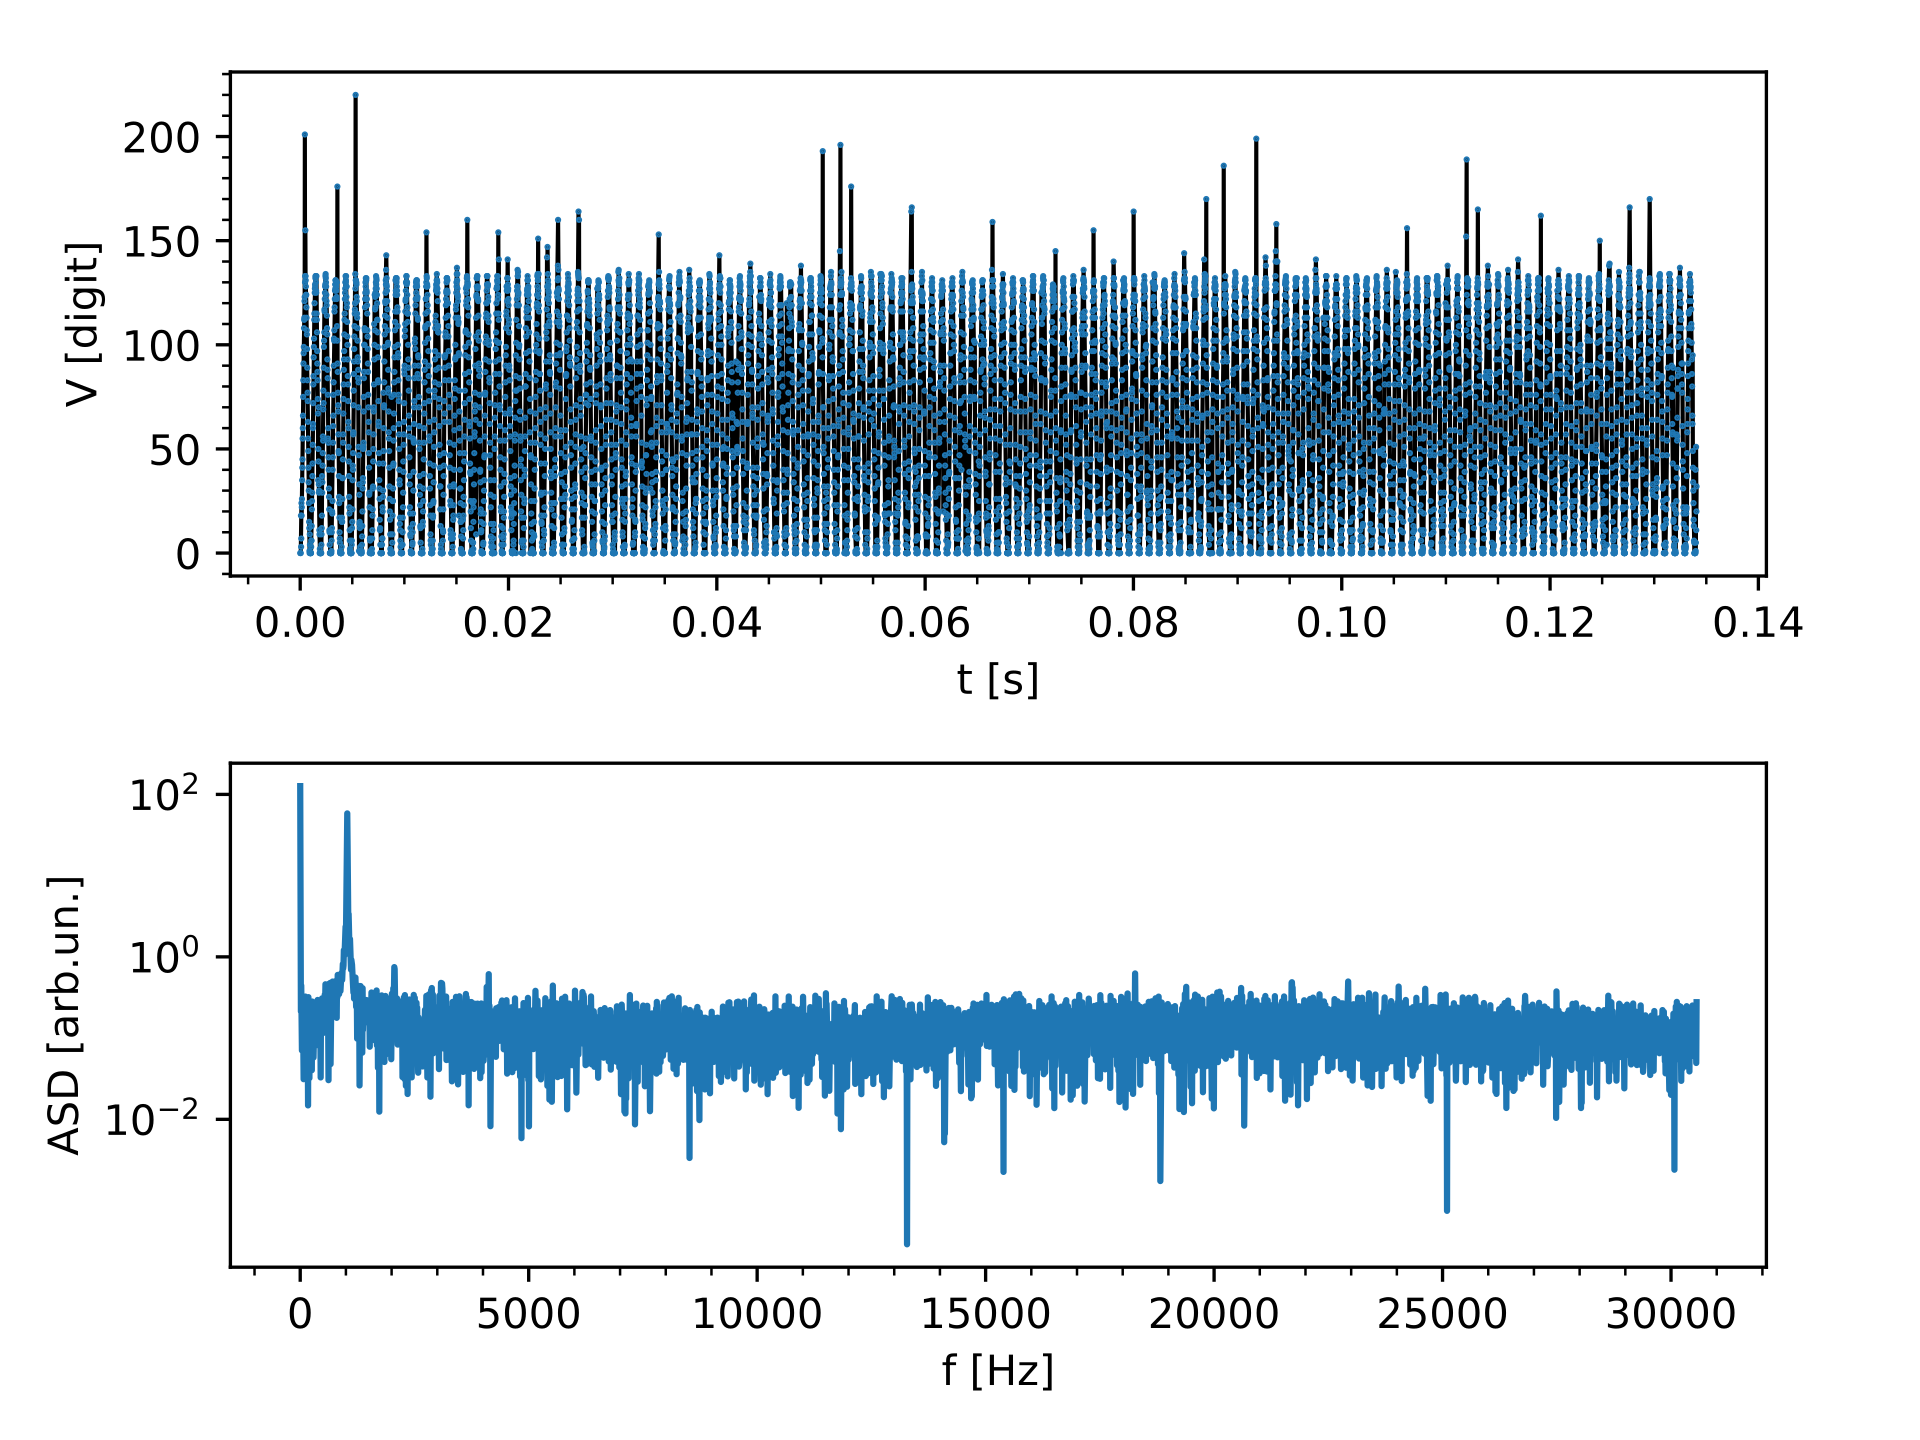
\includegraphics[width=0.45\columnwidth]{img/ese9/dataEDJ-VG-1.75V.png}
    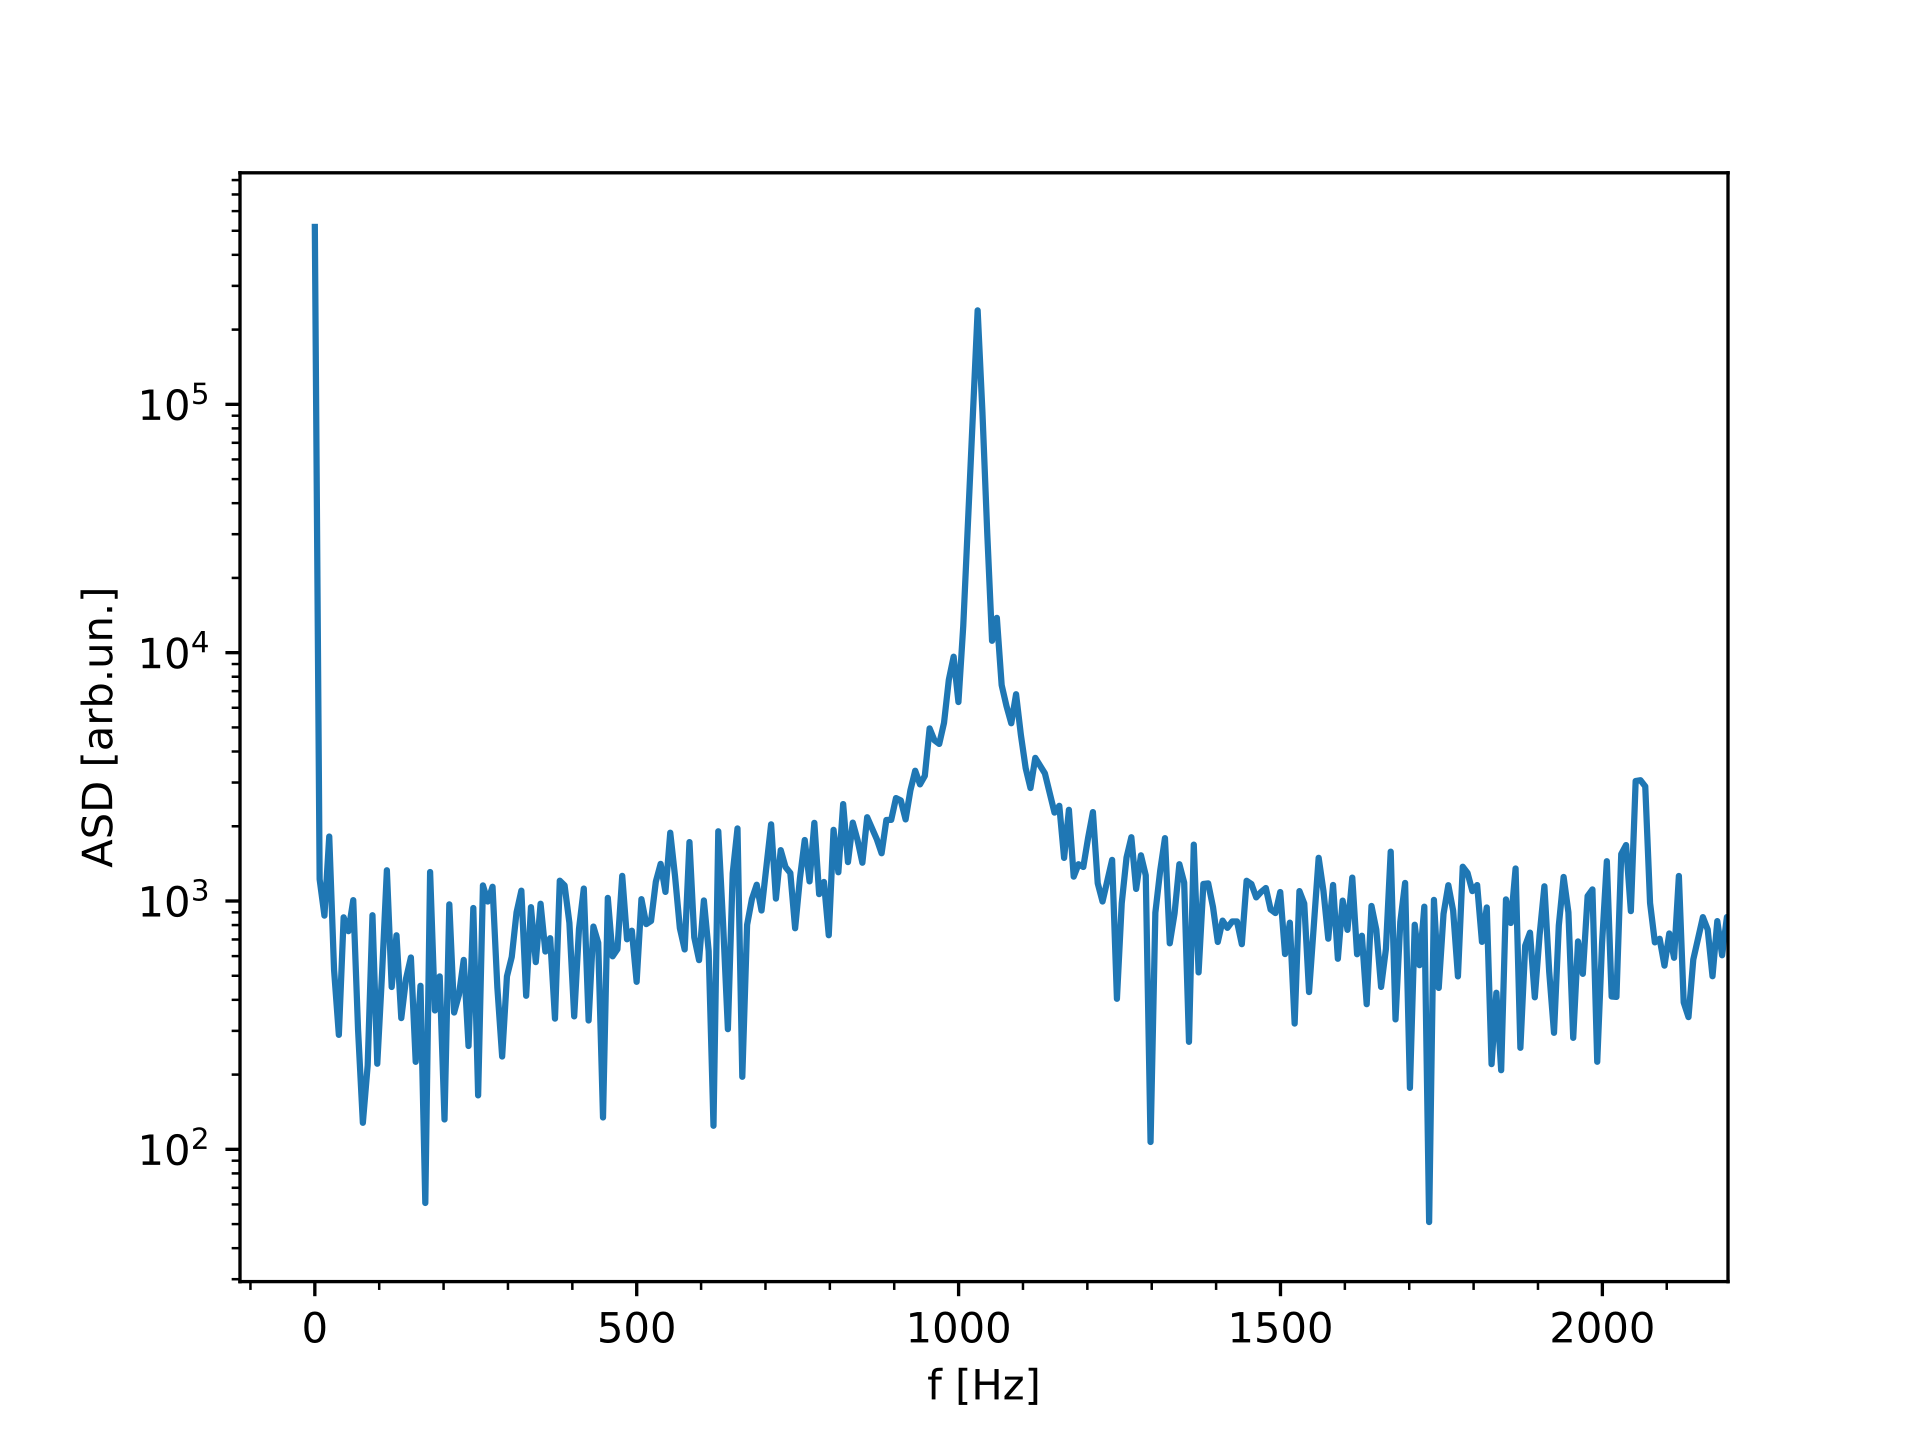
\includegraphics[width=0.48\columnwidth]{img/ese9/dataEDJ-VG-1.75V-tagl.png}
    \caption{Grafici relativi al segnale sinusoidale del generatore. Come atteso, la trasformata presenta un unico picco significativo, a frequenza 1.03 kHz.}
    \label{fig:ese9-VG}
\end{figure}

\begin{figure}[H]
    \centering
    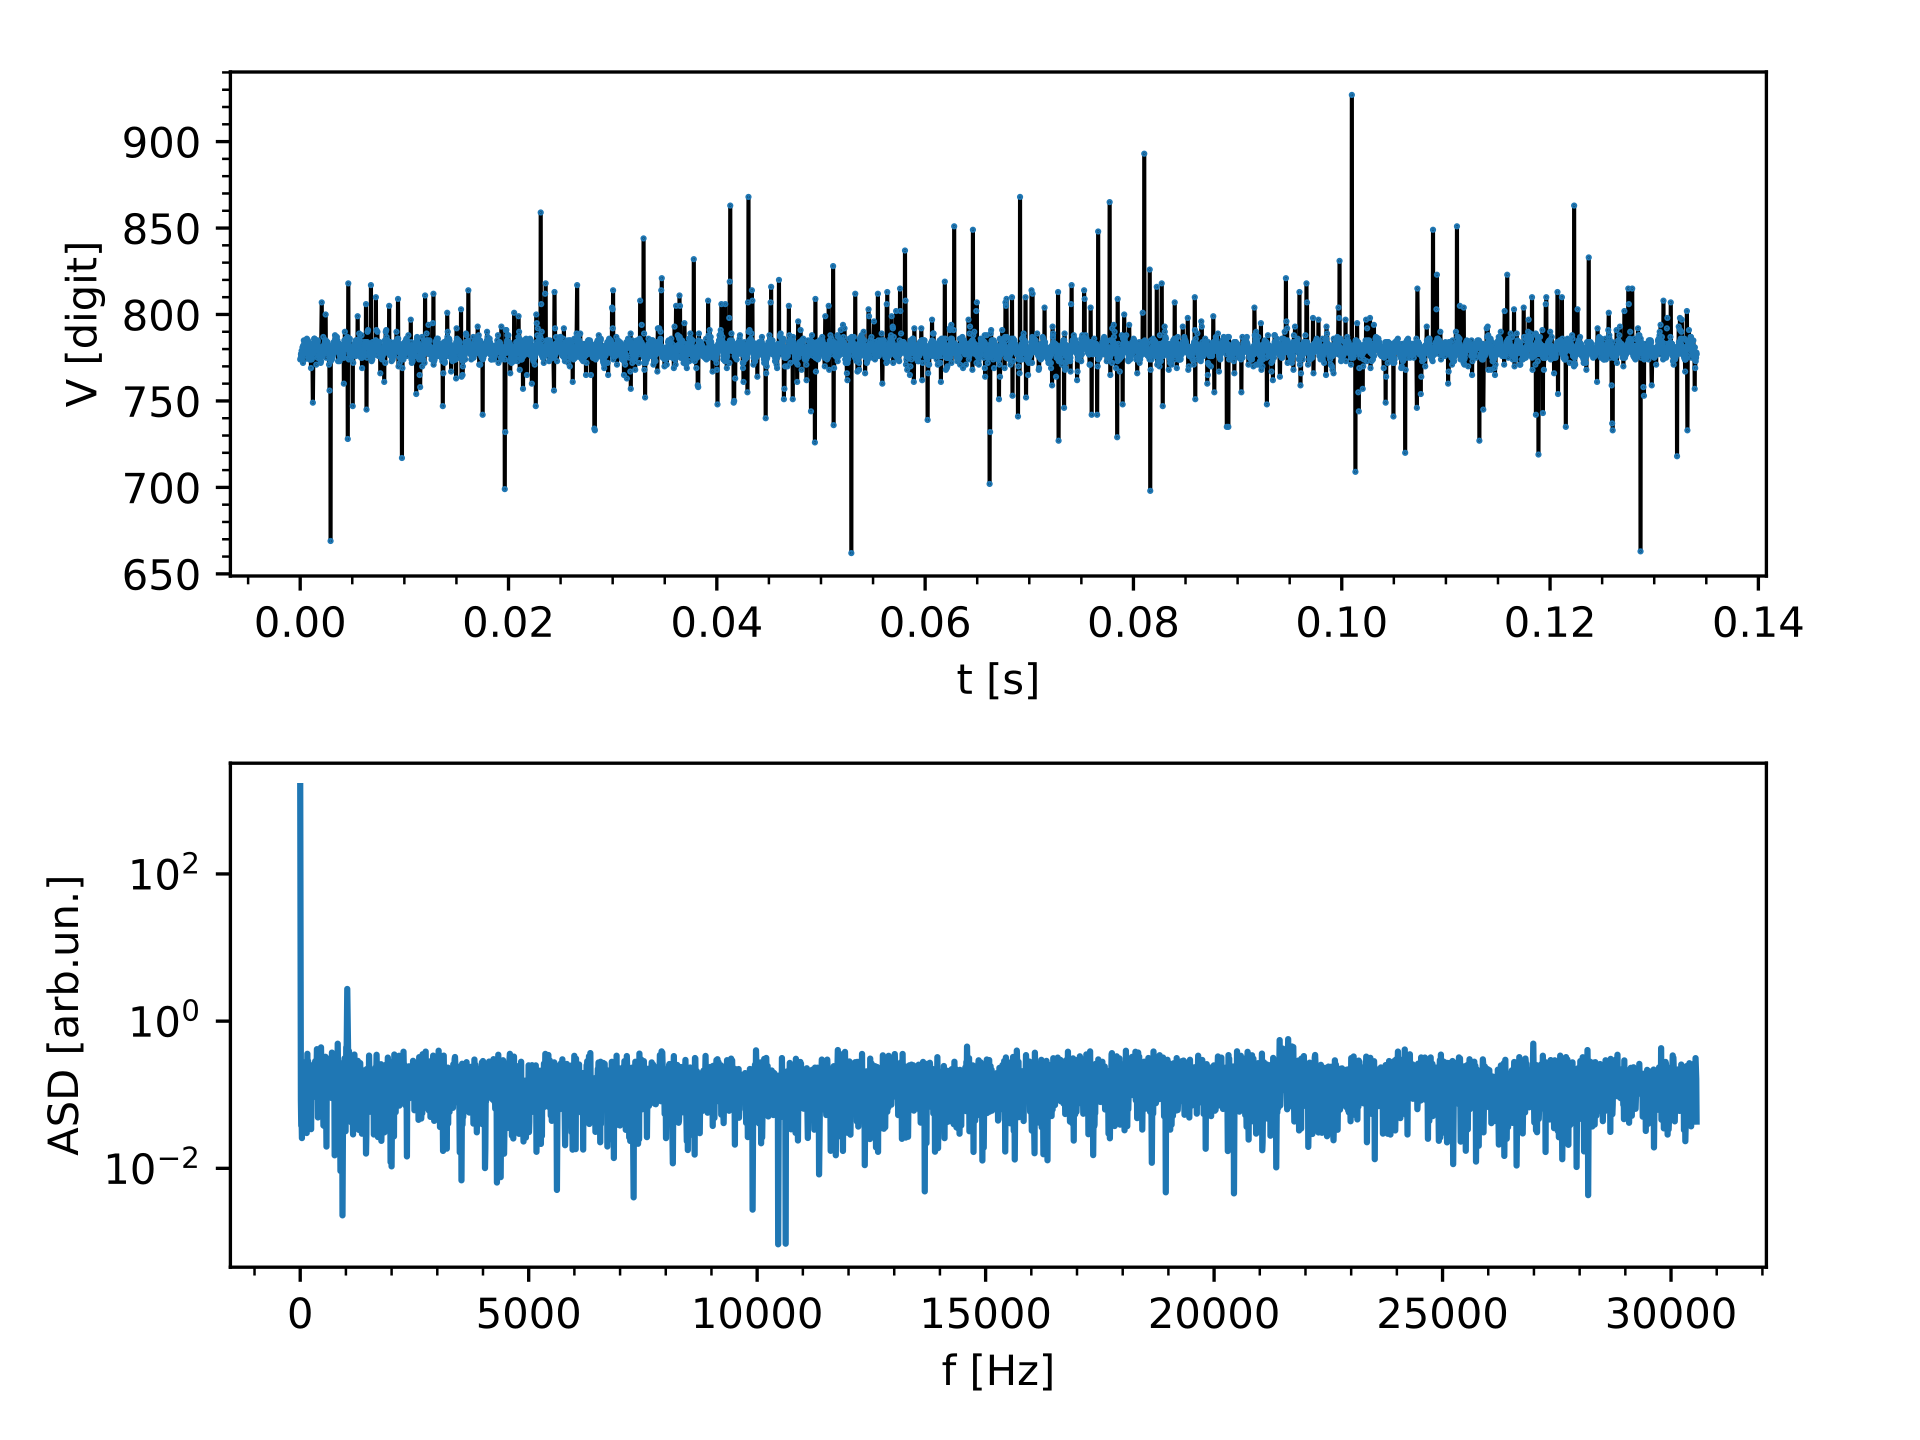
\includegraphics[width=0.45\columnwidth]{img/ese9/dataEDJ-vd-1.75V.png}
    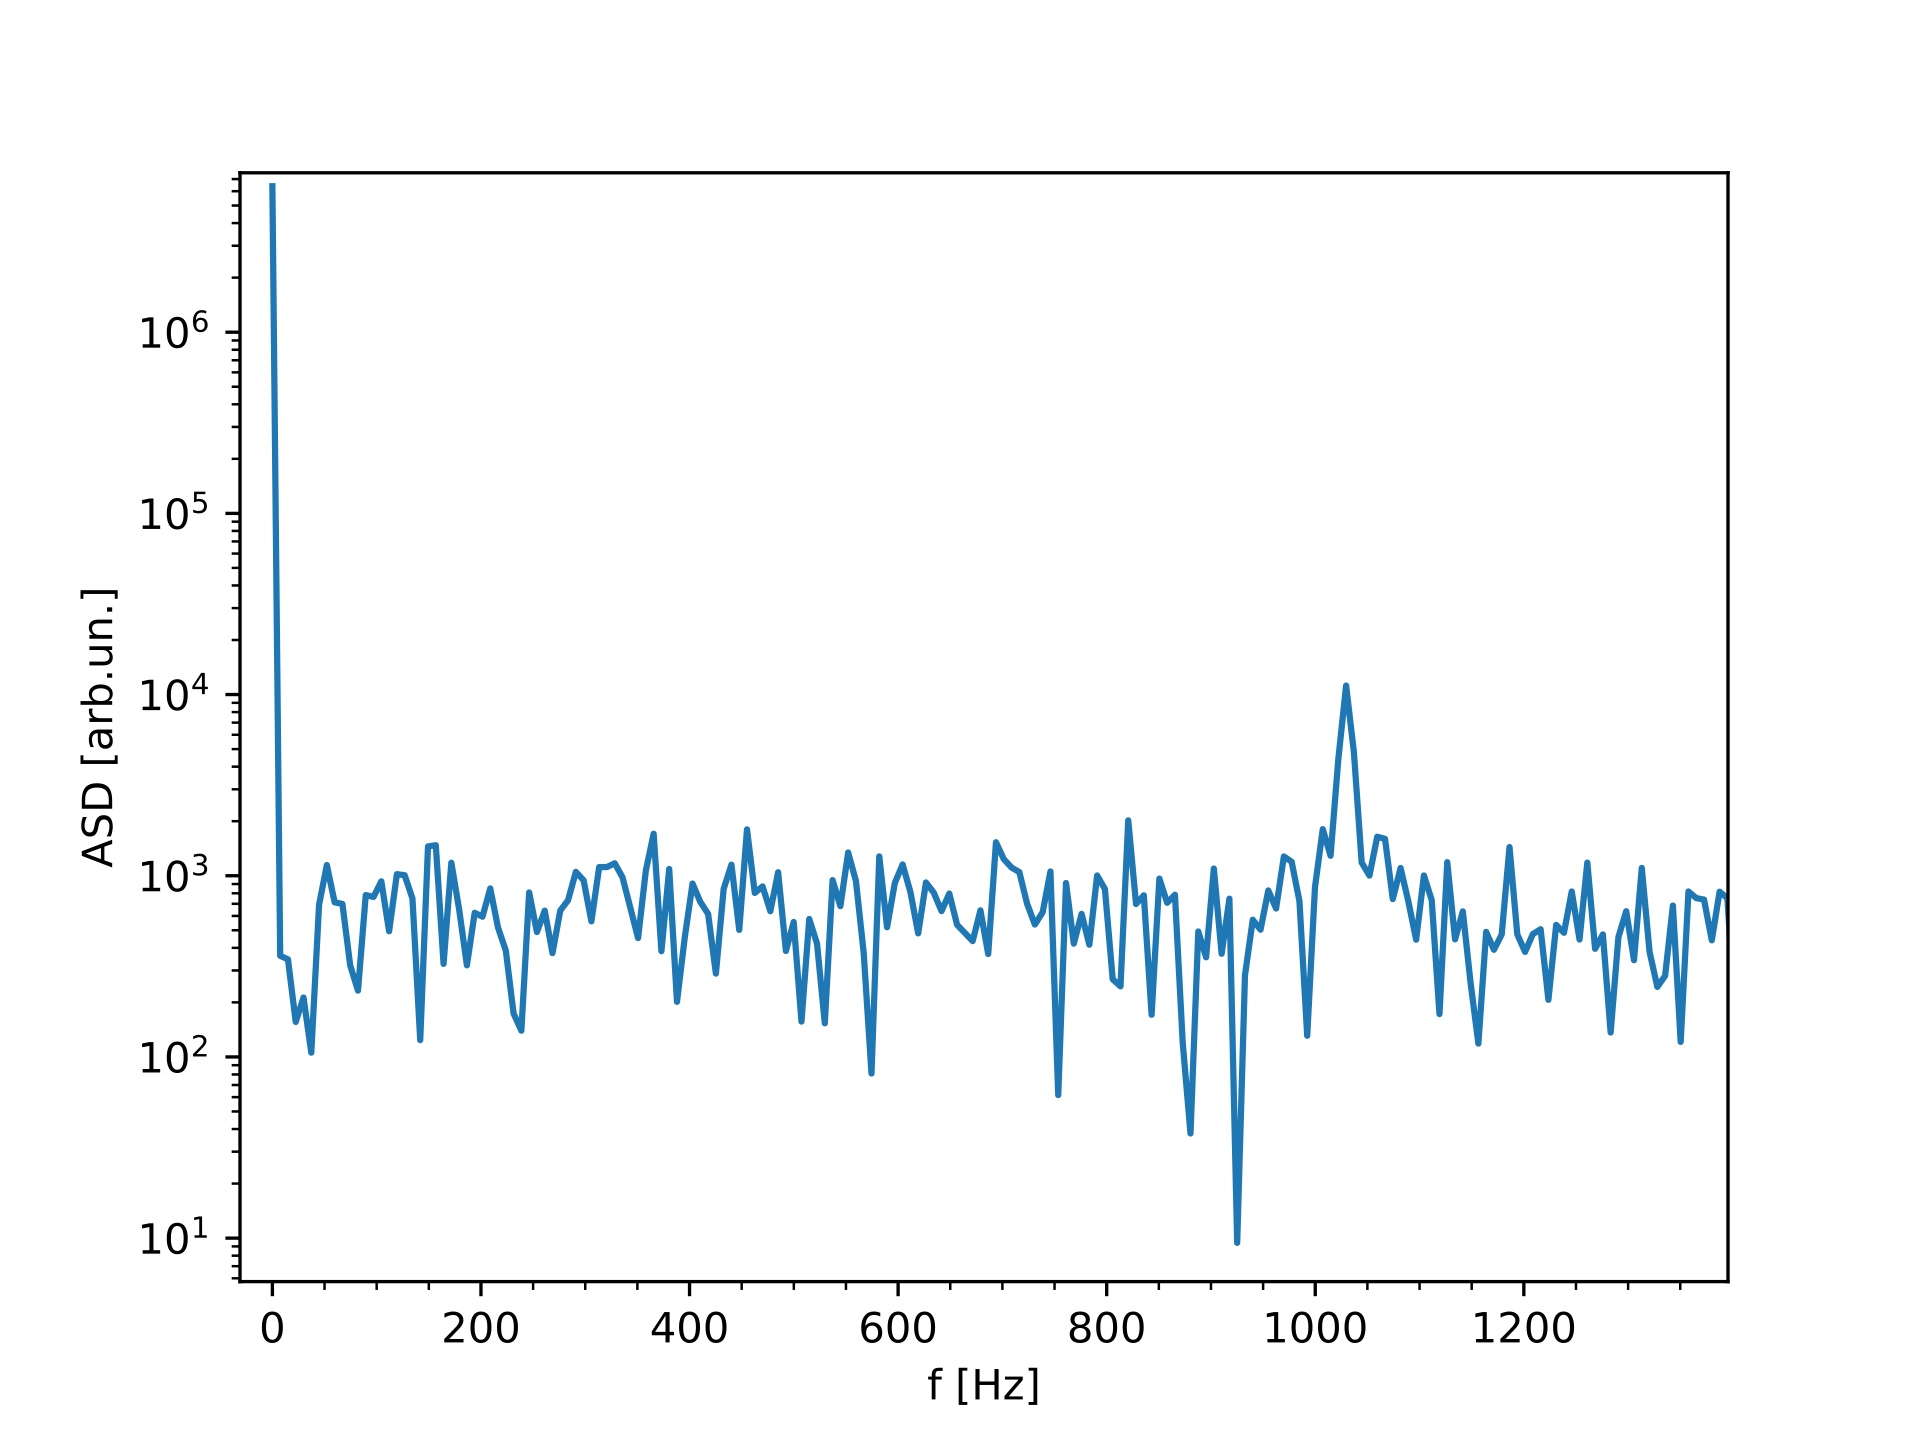
\includegraphics[width=0.48\columnwidth]{img/ese9/dataEDJ-vd-1.75V-tagl.png}
    \caption{Grafici relativi alla d.d.p. ai capi del diodo. Notare il rumore e il picco alla frequenza di 1.03 kHz.}
    \label{fig:ese9-vd}
\end{figure}

\begin{figure}[H]
    \centering
    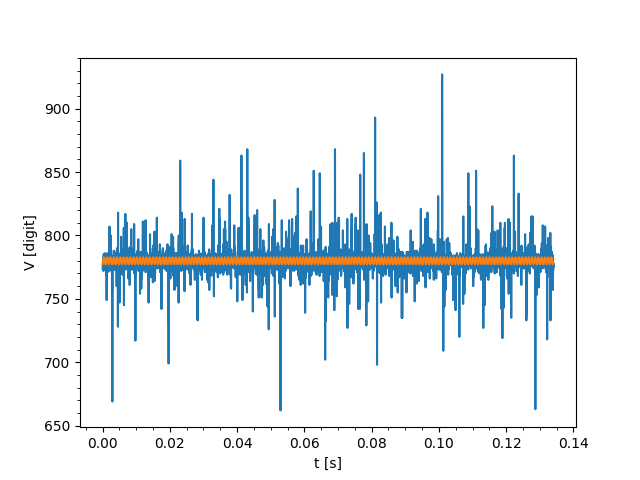
\includegraphics[width=0.45\columnwidth]{img/ese9/dataEDJ-vd-1.75V-lockin.png}
    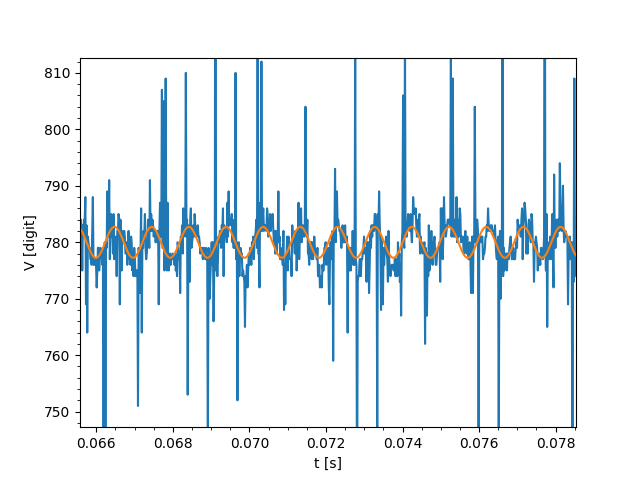
\includegraphics[width=0.45\columnwidth]{img/ese9/dataEDJ-vd-1.75V-lockin-tagl.png}
    \caption{Ricostruzione del segnale, a partire dal valore della trasformata di Fourier nel picco della figura \ref{fig:ese9-vd}. Nel grafico a destra abbiamo effettuato uno zoom su un intervallo casuale per maggiore chiarezza.}
    \label{fig:ese9-lockin}
\end{figure}


\section{Auto-oscillatore con transistor BJT}
In questa esperienza, abbiamo utilizzato un transistor per produrre un auto-oscillatore. In particolare, abbiamo fornito alla base di un transistor a emettitore comune in regime attivo la corrente del collettore, sfasata di mezzo periodo. Questo circuito è a feedback positivo, per cui si inducono spontaneamente oscillazioni.\\
Dai grafici della FFT, notiamo che il picco della fondamentale risulta essere più largo rispetto a quello che ci aspetteremmo per un'onda sinusoidale pura e inoltre notiamo la presenza di armoniche.\\
Il primo effetto potrebbe essere dovuto al fatto che l'auto-oscillatore può oscillare in un range di frequenze; mentre il secondo effetto potrebbe essere causato dalla dipendenza non lineare fra  tensione e corrente nella curva caratteristica di base del transistor, che porta ad un comportamento ``asimmetrico" dell'amplificatore.\\
Per una maggiore leggibilità, abbiamo preferito riportare solamente il grafico della FFT zoomato sull'intorno della regione di nostro interesse.

\begin{figure}[H]
    \centering
    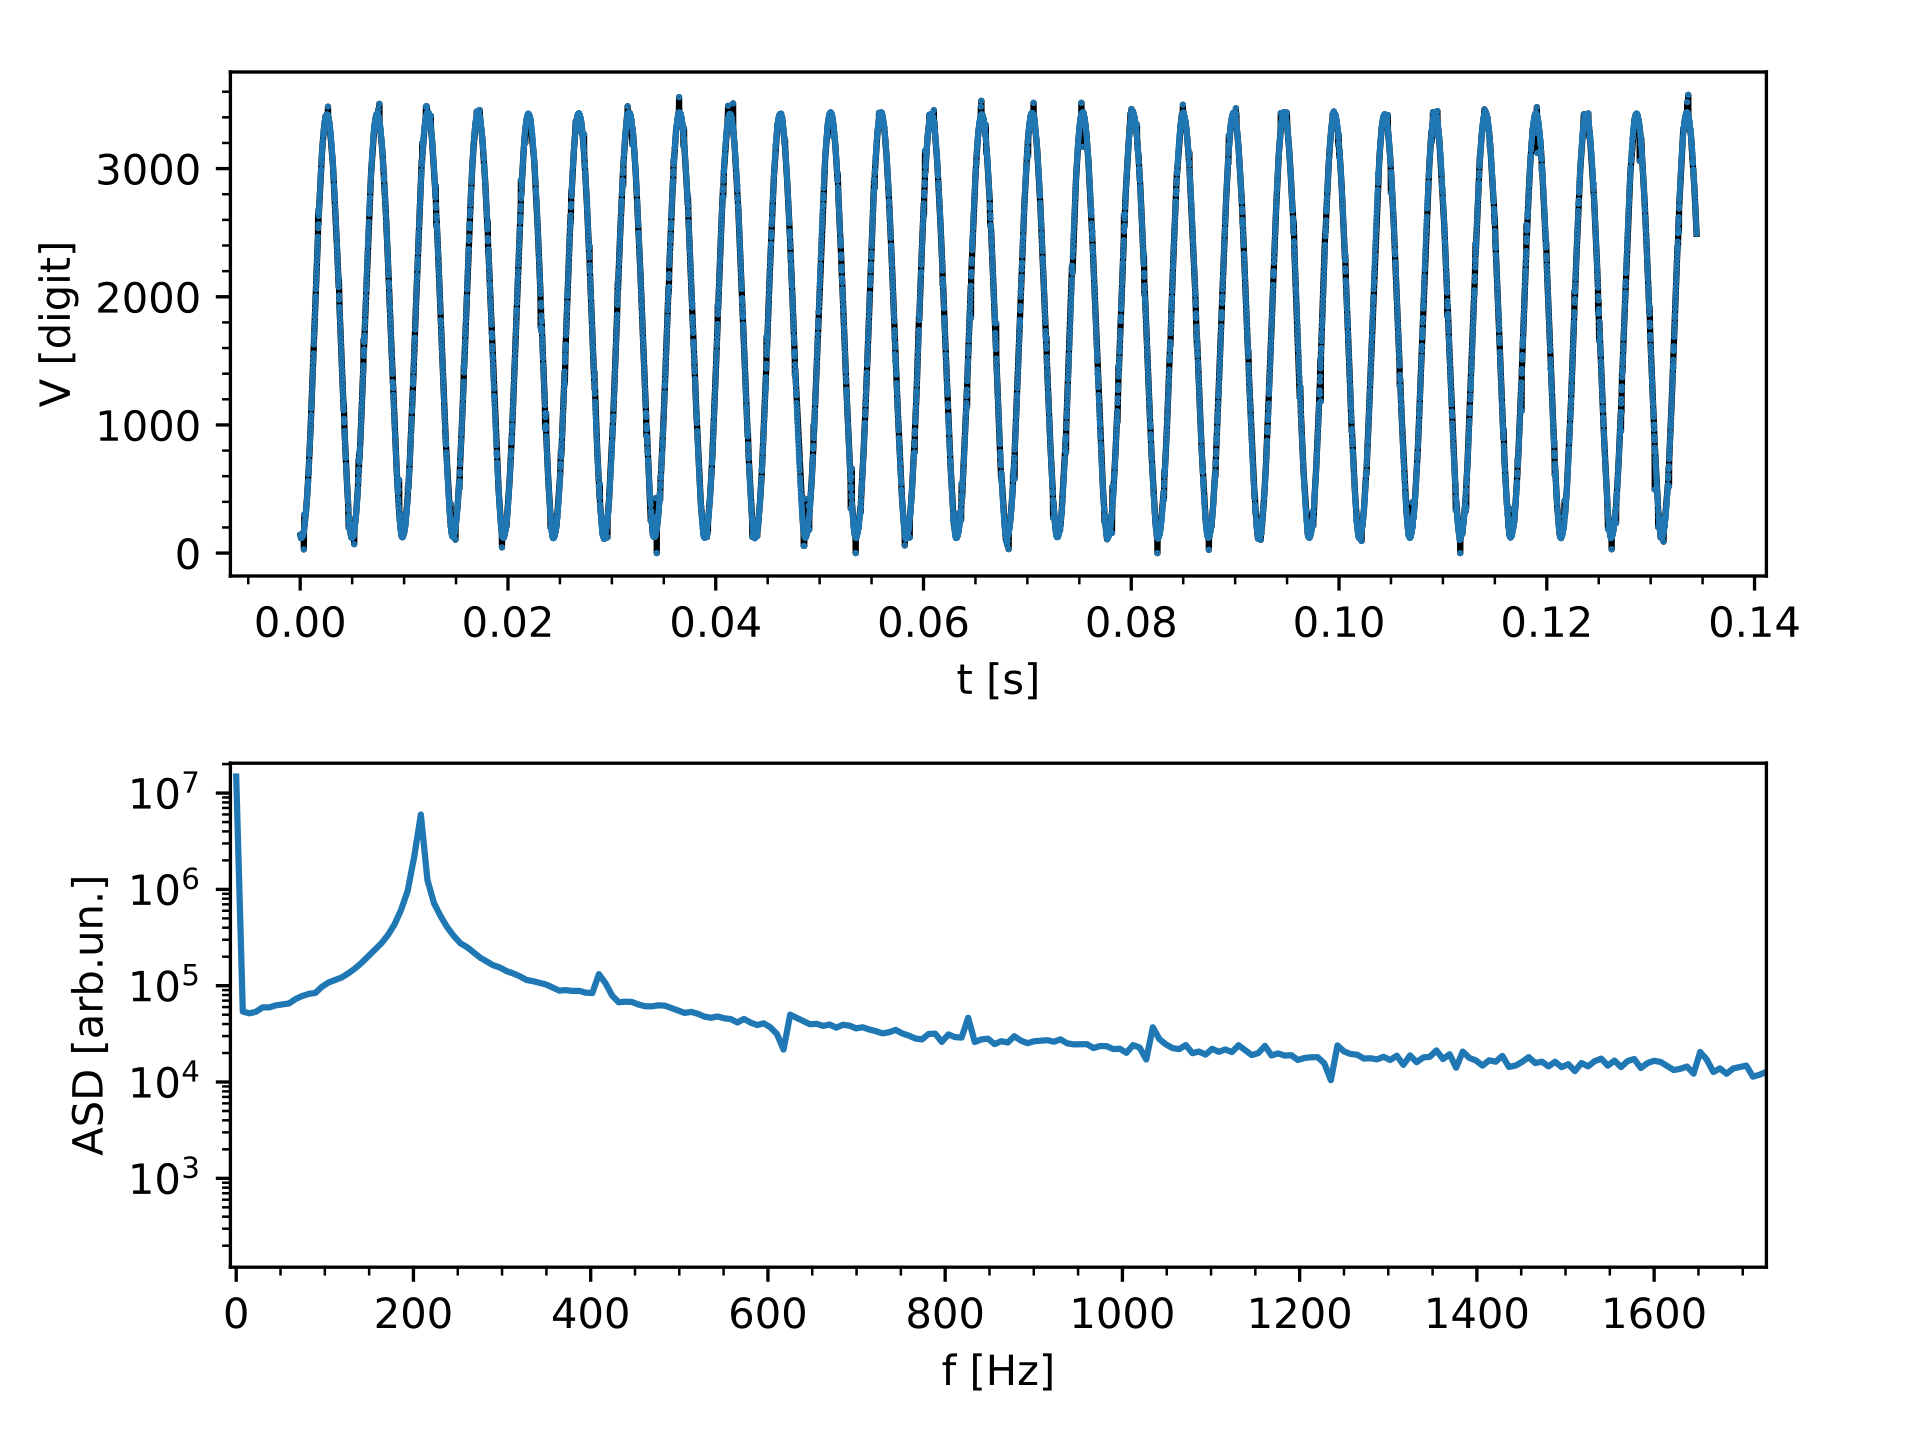
\includegraphics[width=0.48\columnwidth]{img/ese11/16.6uA-10us.png}
    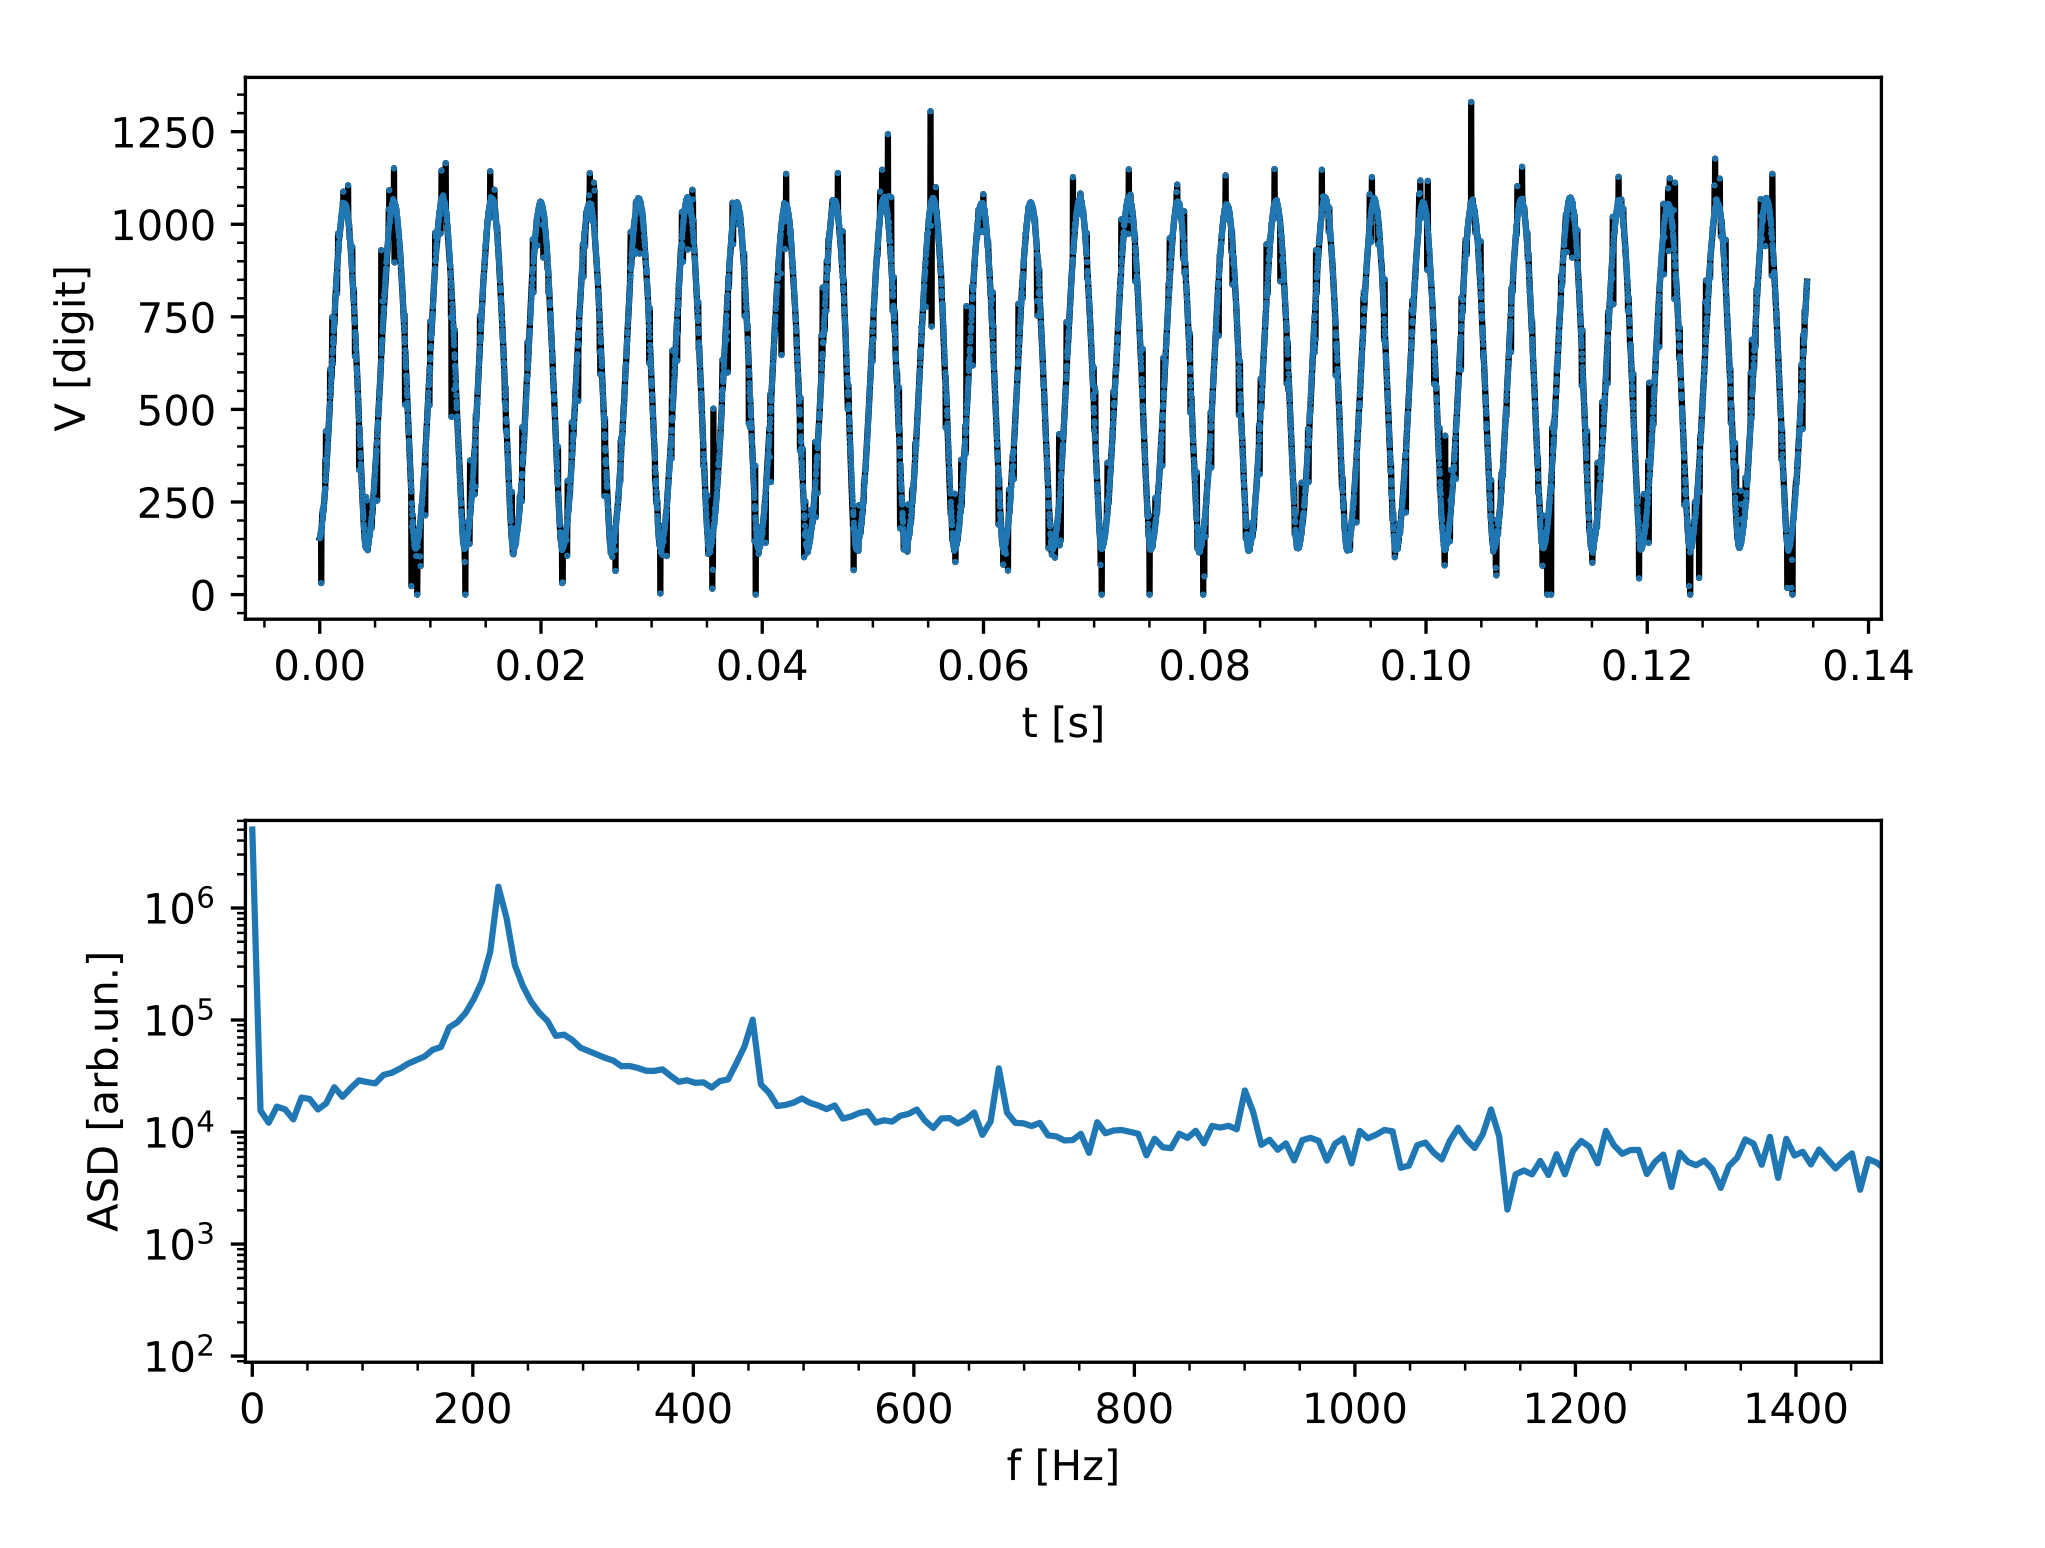
\includegraphics[width=0.48\columnwidth]{img/ese11/24.5uA-10us.png}
    \caption{Grafici relativi a due diverse acquisizioni a corrente di base fornita dal generatore rispettivamente di ($16.6 \pm 0.2$) $\mu$A e ($24.5 \pm 0.2$) $\mu$A.}
    \label{fig:ese11}
\end{figure}


\section{Oscillatore smorzato RLC}
In questa esperienza abbiamo costruito un circuito RLC, che si comporta come un oscillatore armonico smorzato. Abbiamo utilizzato un induttore, formato da una coppia di avvolgimenti, di resistenza interna (39.7 $\pm$ 0.6) $\Omega$ e condensatori con diverse capacità. Abbiamo acquisito la d.d.p. ai capi del condensatore, prima cambiando il condensatore e lasciando gli avvolgimenti dell'induttore collegati in serie; successivamente cambiando gli avvolgimenti dell'induttore lasciando il condensatore a capacità ($0.1 \pm 10\%$) $\mu$F.\\
Analogamente alla sezione precedente, abbiamo preferito riportare solamente il grafico della FFT zoomato sull'intorno del picco di nostro interesse.\\
Notiamo che lo spettro presenta un picco attorno alla frequenza di risonanza, la cui larghezza dipende dal fattore di qualità, ovvero dallo smorzamento dell'oscillatore. In particolare, ci aspettiamo che valga:
\[\tau \simeq \frac{\sqrt{3}}{\pi \Delta f_{\text{fwhm}}} \]
dove $\tau$ è il tempo caratteristico dello smorzamento.\\
Abbiamo stimato $\tau$ e $T$ (periodo dell'oscillazione) a partire dai grafici delle FFT. A causa della scarsa risoluzione delle frequenze, il valore di $\Delta f_{\text{fwhm}}$ è particolarmente difficile da stimare con precisione, per cui per i valori di $\tau$ abbiamo preferito stimare un intervallo ragionevole che contenesse il valore atteso. Per stimare tale intervallo, abbiamo preso il valore massimo fra i due vicini al picco, ottenendo una sottostima $A_m$ del valore del picco, e prolungando i segmenti della spezzata ai lati del picco abbiamo ottenuto una sovrastima $A_M$ del valore del picco $A_M$. Abbiamo poi usato sia $A_m/2$ che $A_M/2$ per calcolare gli estremi dell'intervallo in cui è presente $\Delta f_{\text{fwhm}}$. Da questi valori abbiamo ottenuto una stima di $\tau$. \\
Riportiamo i valori di $\tau$ e di $T$, stimati dalle FFT e ottenuti dai best-fit eseguiti in laboratorio, facendo presente che abbiamo ritenuto opportuno non assegnare un errore a $T$, in quanto non abbiamo attribuito incertezze alle FFT:\\
\begin{center}
    \begin{tabular}{|c||c|c||c|c|}
    \hline
    \multicolumn{5}{|c|}{Avvolgimenti in serie, capacità variabile}\\
    \hline
        Capacità $C$ & $T$ da FFT & $T$ da fit & $\tau$ da FFT & $\tau$ da fit\\
    \hline\hline
        ($0.1  \pm 10 \%$) $\mu$F & 1.56 ms & (1.55470 $\pm$ 0.00002) ms & (17.5 $\pm$ 0.5) ms & (17.07 $\pm$ 0.01) ms\\
    \hline
        ($0.22 \pm 10 \%$) $\mu$F & 2.22 ms & (2.23467 $\pm$ 0.00001) ms & (23 $\pm$ 3) ms & (20.038 $\pm$ 0.006) ms\\
    \hline
        ($0.47 \pm 10 \%$) $\mu$F & 3.17 ms & (3.16472 $\pm$ 0.00003) ms & (27 $\pm$ 7) ms & (22.018 $\pm$ 0.009) ms\\
    \hline
    \end{tabular}
    \\\quad
    \newline
    \begin{tabular}{|c||c|c||c|c|}
    \hline
    \multicolumn{5}{|c|}{Capacità fissa $C = $($0.1  \pm 10 \%$) $\mu$F, avvolgimenti variabili}\\
    \hline
        Avvolgimenti & $T$ da FFT & $T$ da fit & $\tau$ da FFT & $\tau$ da fit\\
    \hline\hline
        Parallelo & 0.708 ms & (0.708981 $\pm$ 0.000005) ms & (8.9 $\pm$ 0.8) ms & (8.4873 $\pm$ 0.0004) ms\\
    \hline
        Anti-parallelo & 0.310 ms & (0.30976 $\pm$ 0.00002) ms & (2.0 $\pm$ 0.1) ms & (2.064 $\pm$ 0.005) ms\\
    \hline
        Anti-serie & 0.6 ms & (0.68365 $\pm$ 0.00002) ms & (3.7 $\pm$ 0.1) ms & (3.655 $\pm$ 0.004) ms\\
    \hline
        Avv. interno & 0.708 ms & (0.707951 $\pm$ 0.000006) ms & (8 $\pm$ 1) ms & (8.242 $\pm$ 0.005) ms\\
    \hline
        Avv. esterno & 0.972 ms & (0.971941 $\pm$ 0.00006) ms & (9 $\pm$ 2) ms & (10.761 $\pm$ 0.004) ms\\
    \hline
    \end{tabular}
\end{center}
Da questi valori, notiamo che c'è accordo tra i valori ottenuti dalla FFT e dai fit. 

\begin{figure}[H]
    \centering
    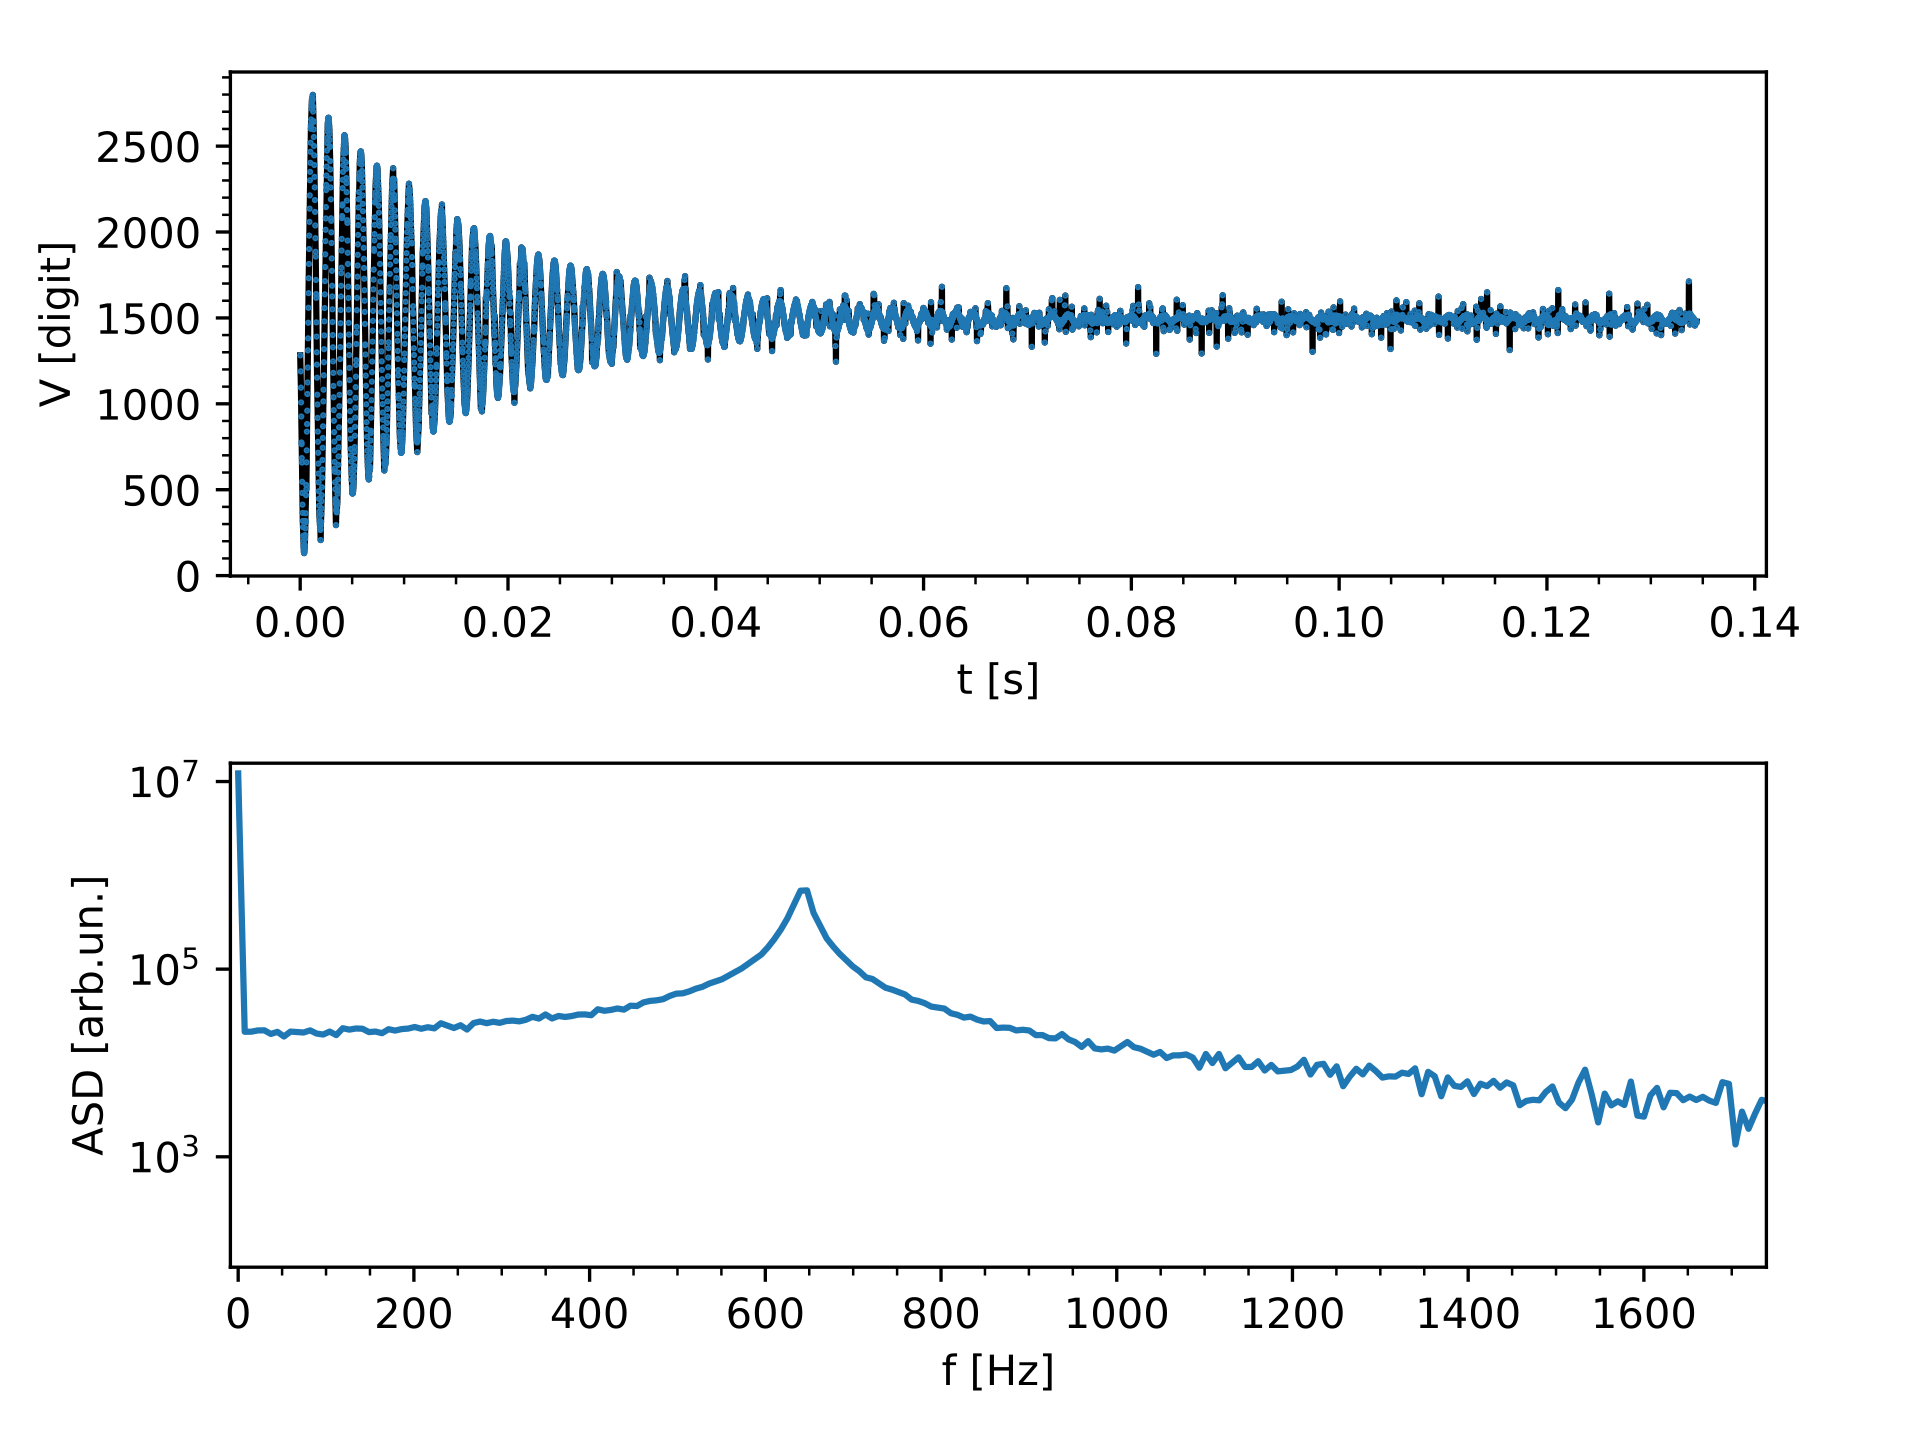
\includegraphics[width=0.45\columnwidth]{img/ese12/0.1uF-non_mediati.png}
    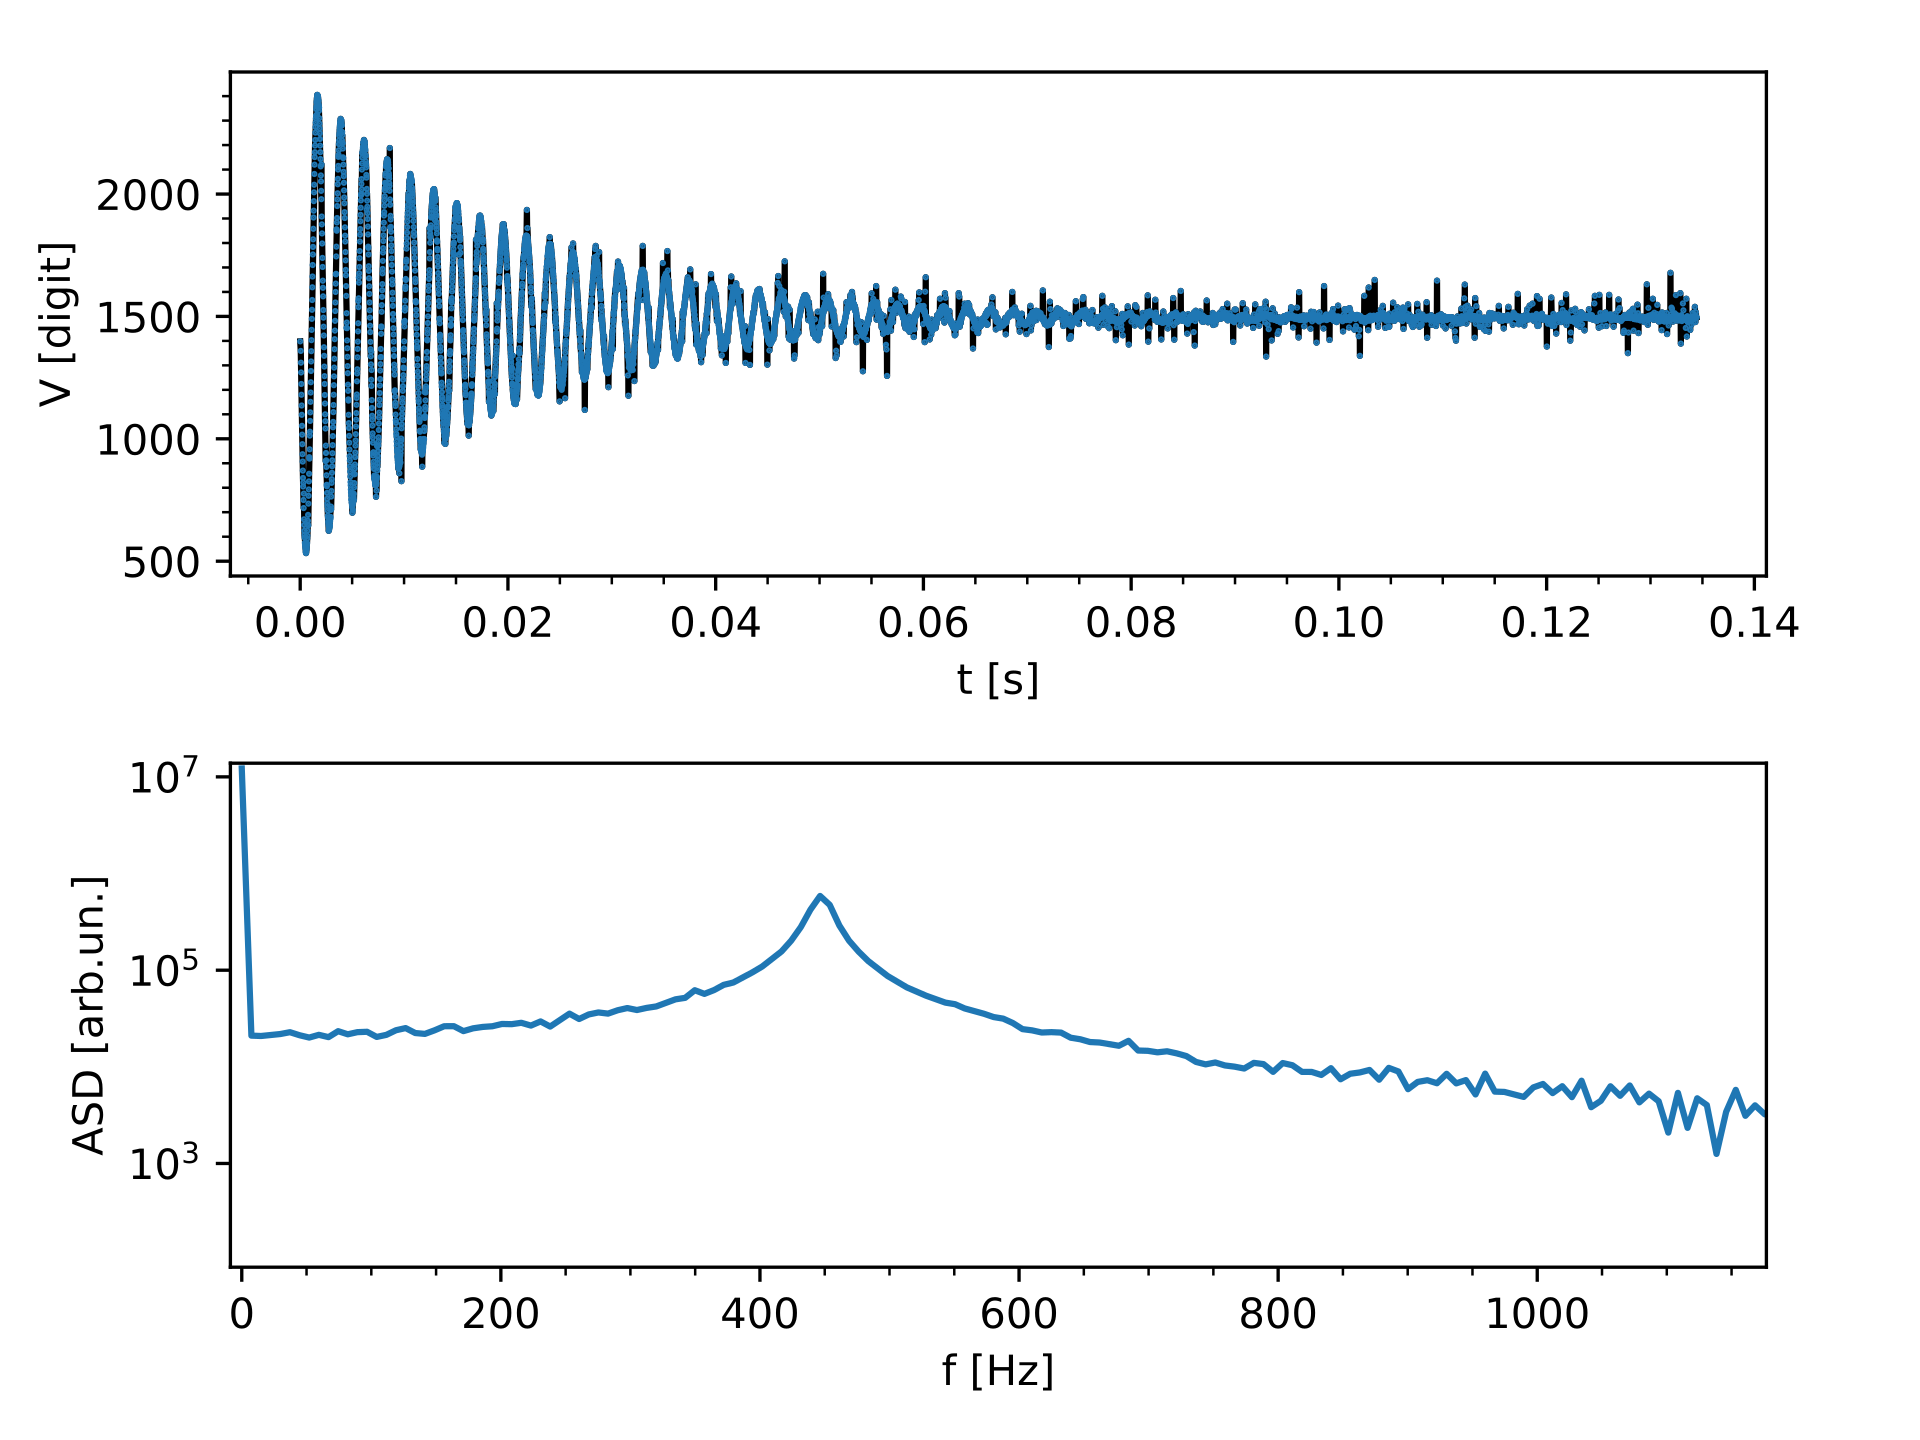
\includegraphics[width=0.45\columnwidth]{img/ese12/0.22uF-non_mediati.png}
    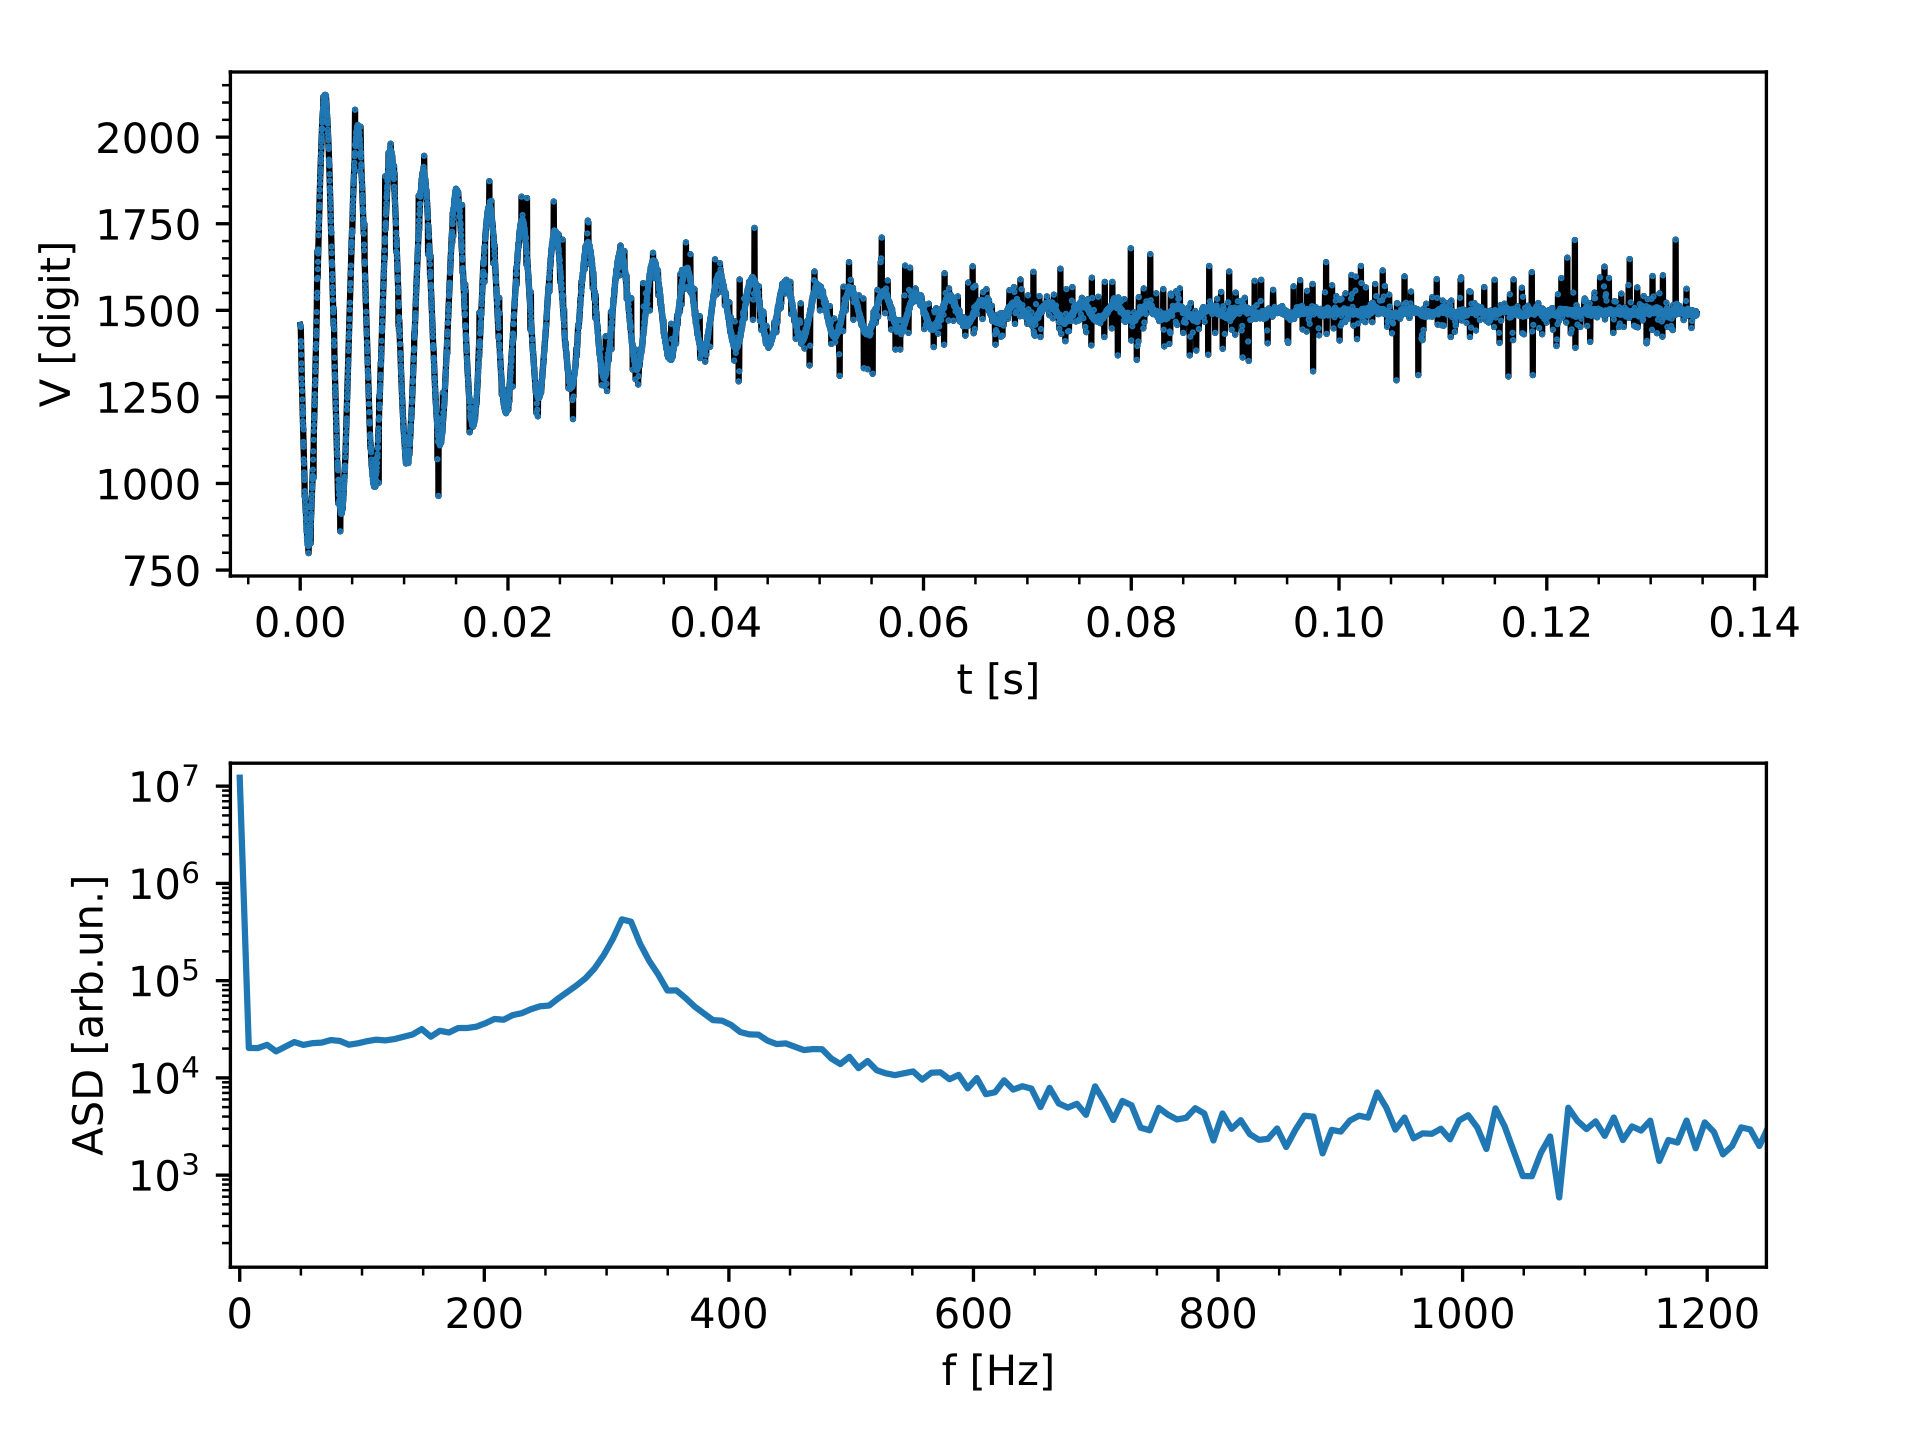
\includegraphics[width=0.50\columnwidth]{img/ese12/0.47uF-non_mediati.png}
    \caption{Dati e zoom della FFT attorno al `picco di risonanza', al variare del valore della capacità del condensatore, con induttanza in serie. Da sinistra a destra: $(0.1 \pm 10\%)$ $\mu$F; $(0.22 \pm 10 \%)$ $\mu$F; ($0.47 \pm 10\%$) $\mu$F.}
    \label{fig:ese12 - capacità differenti}
\end{figure}

\begin{figure}[H]
    \centering
    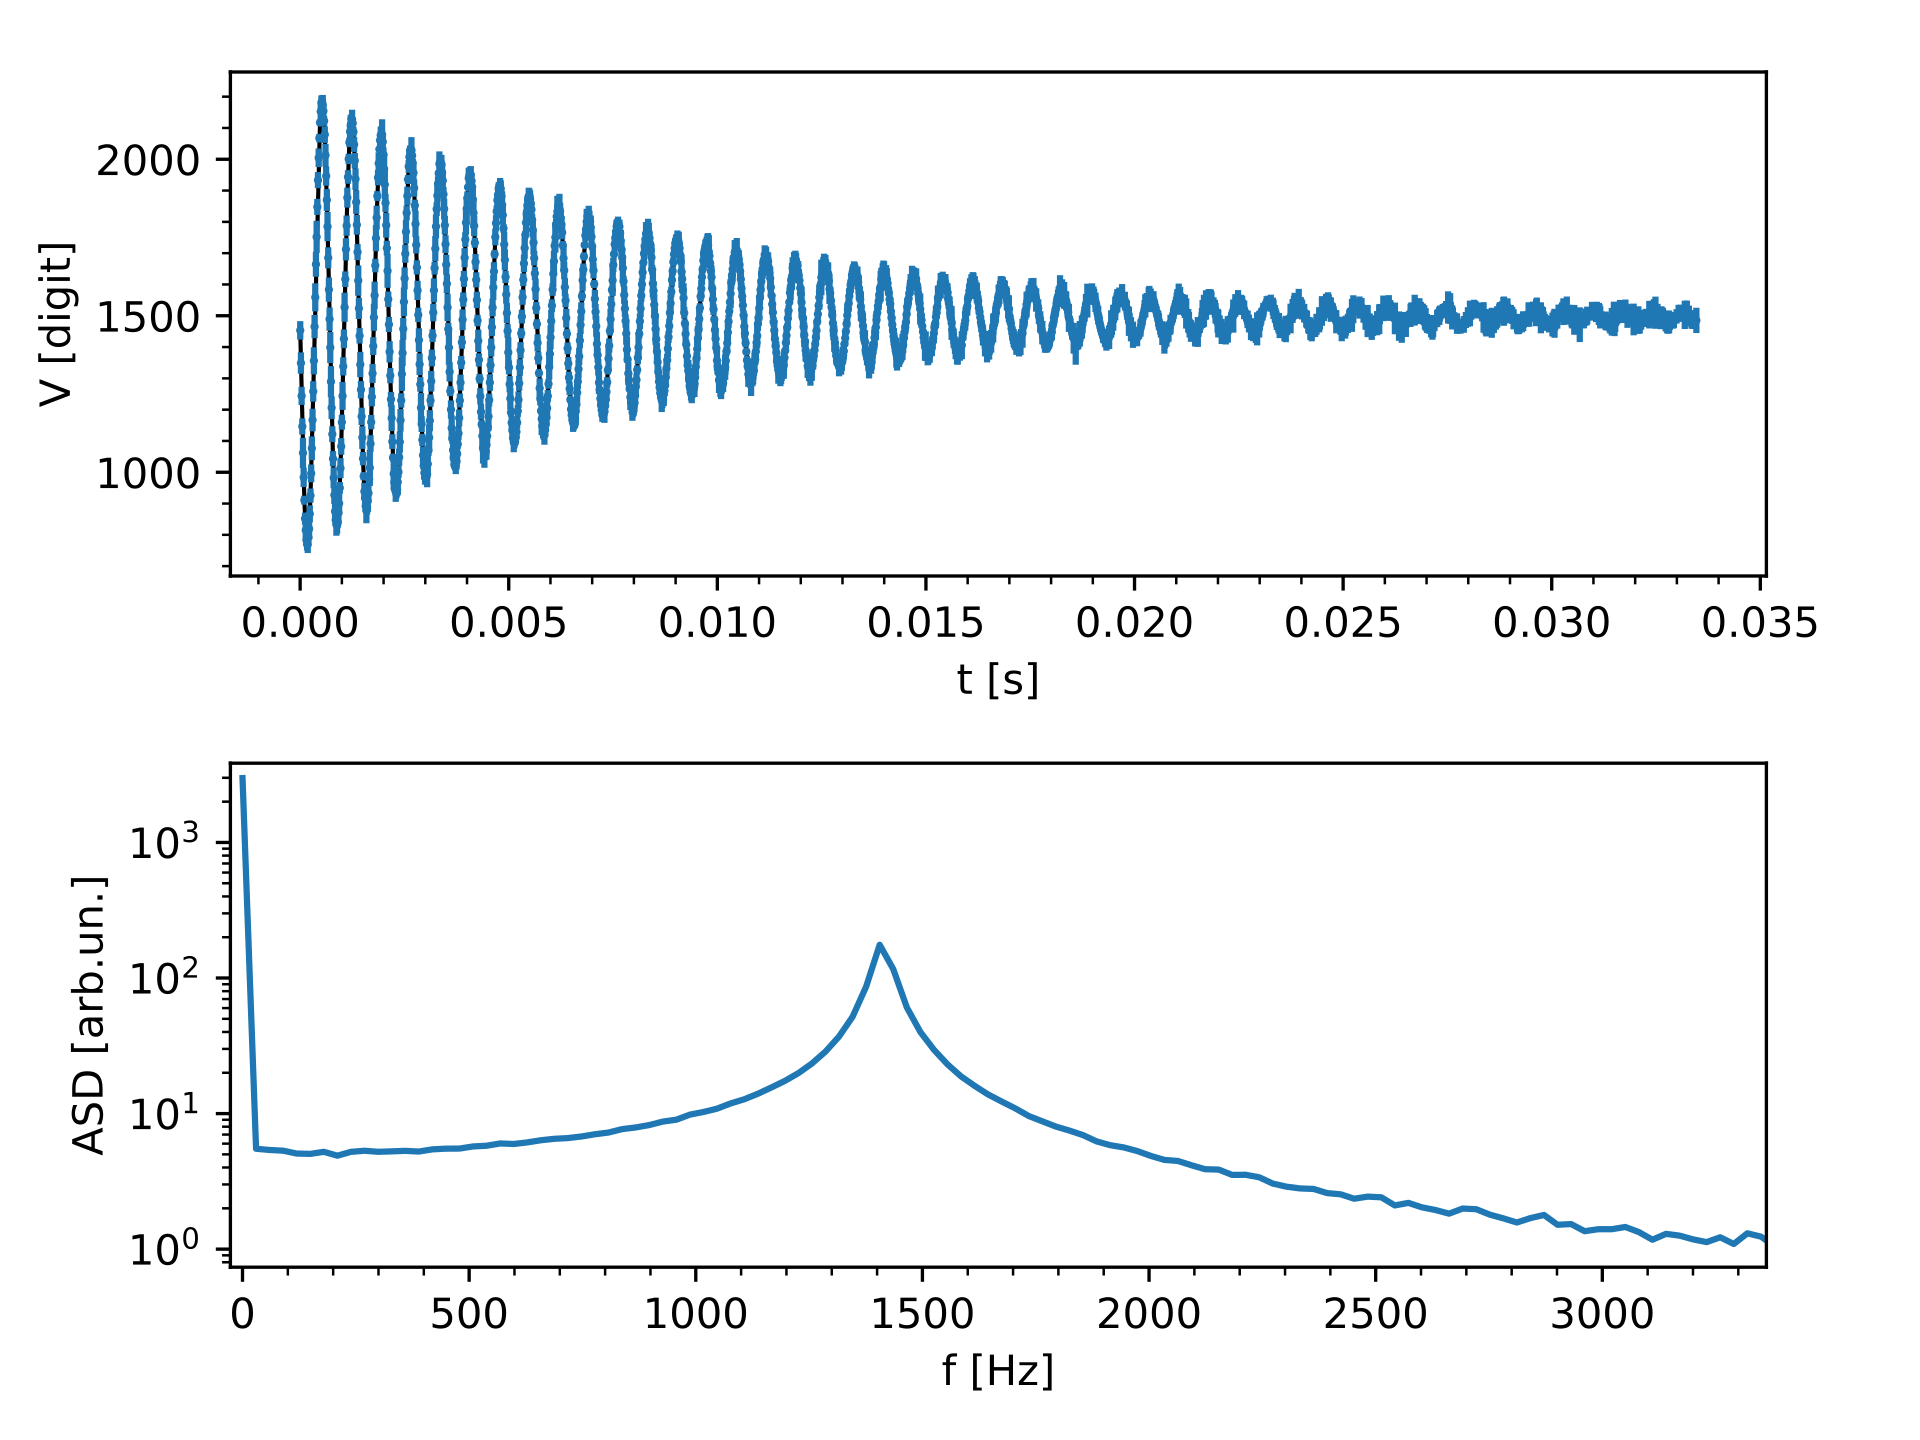
\includegraphics[width=0.45\columnwidth]{img/ese12/ind_par.png}
    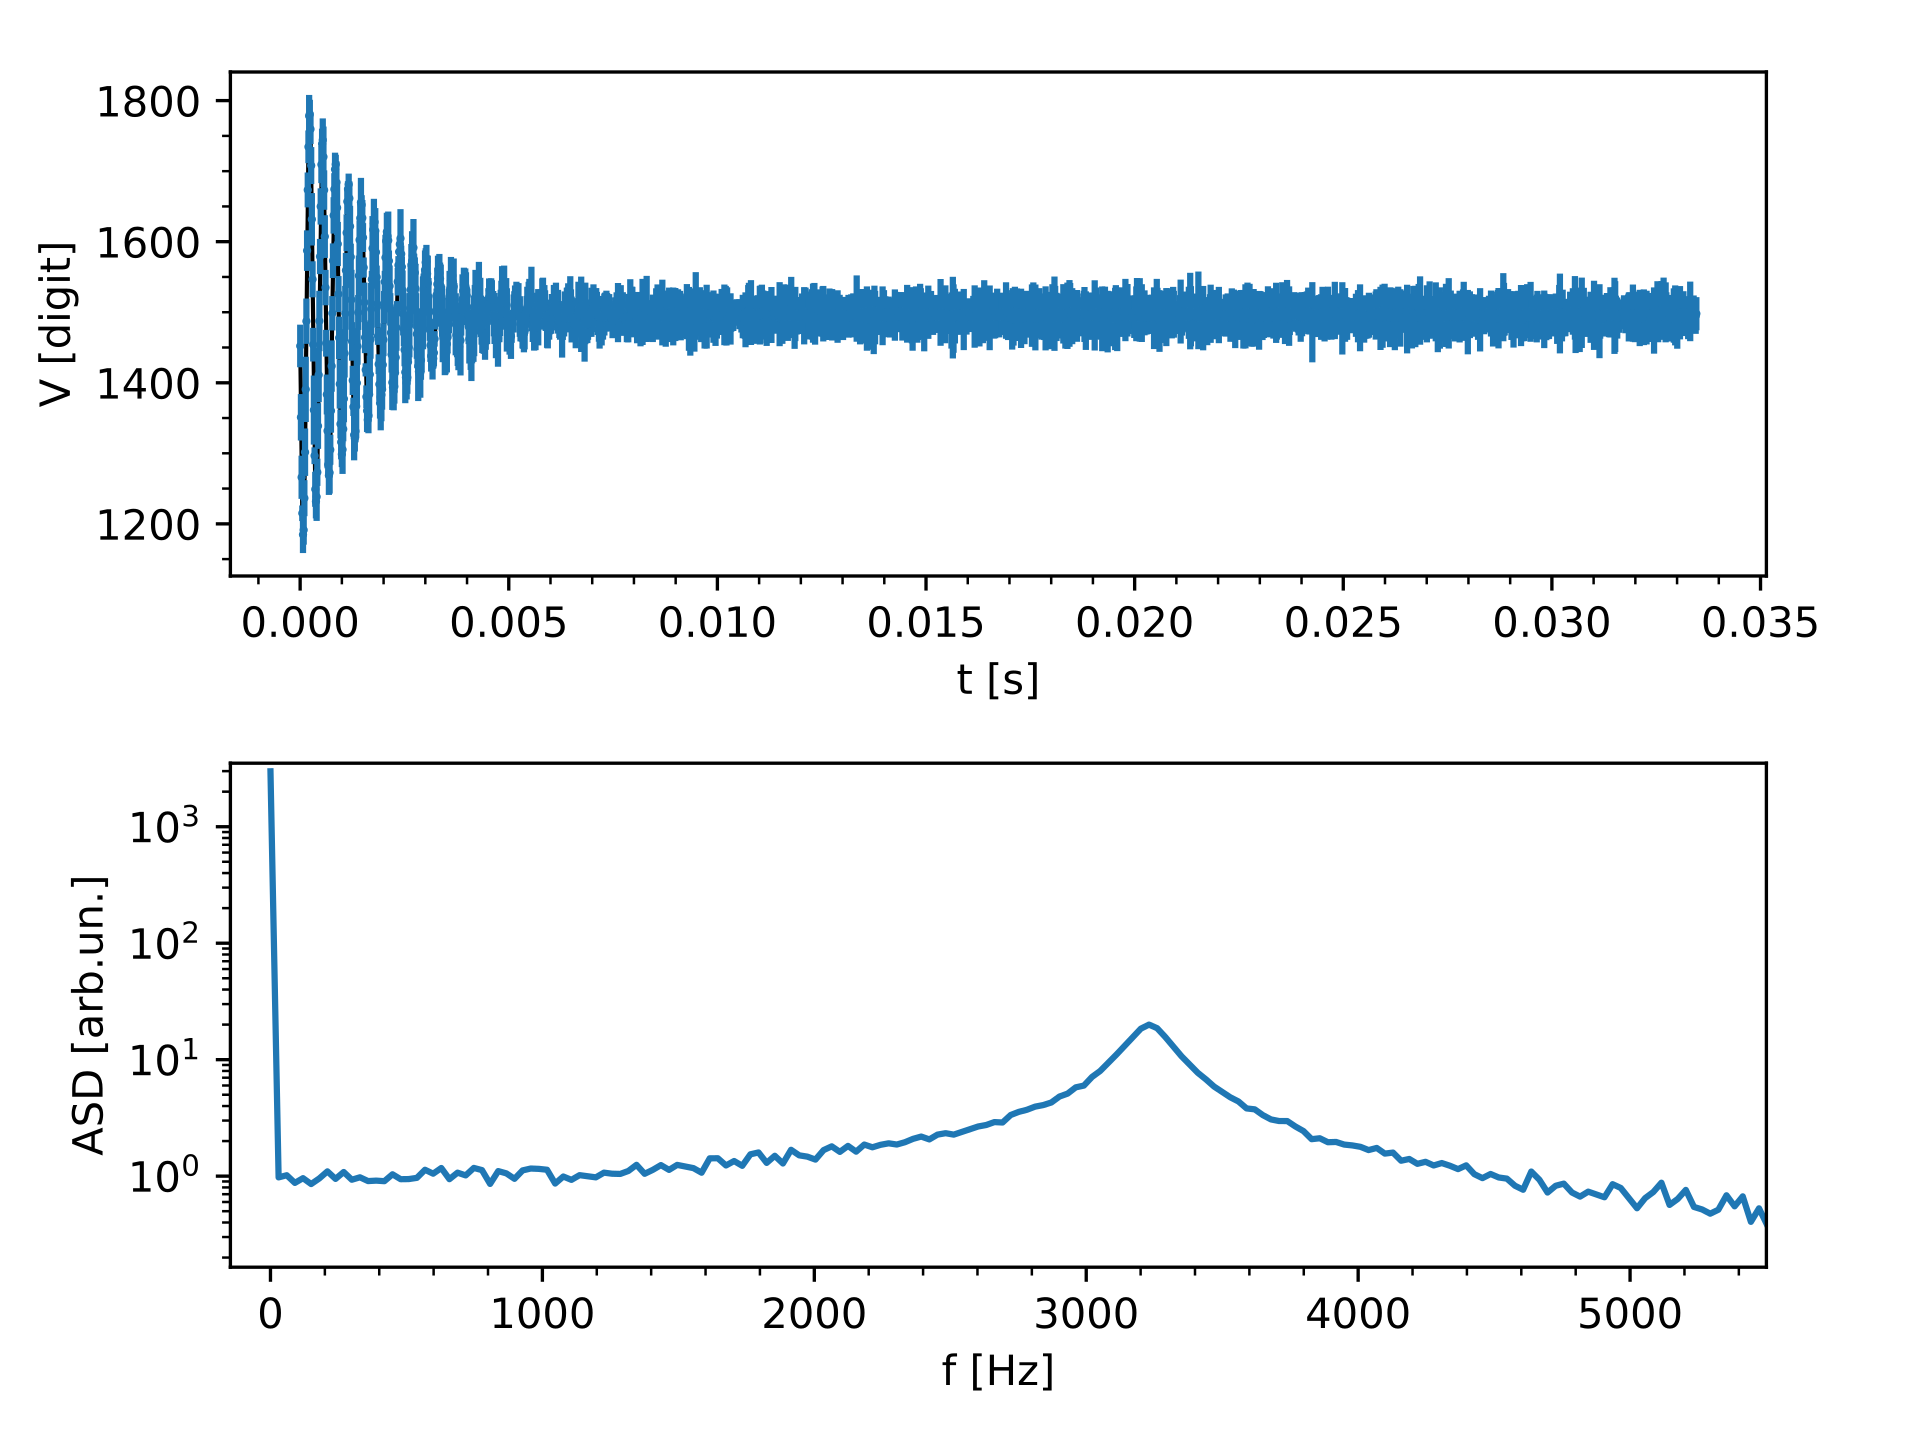
\includegraphics[width=0.45\columnwidth]{img/ese12/ind_antip.png}
    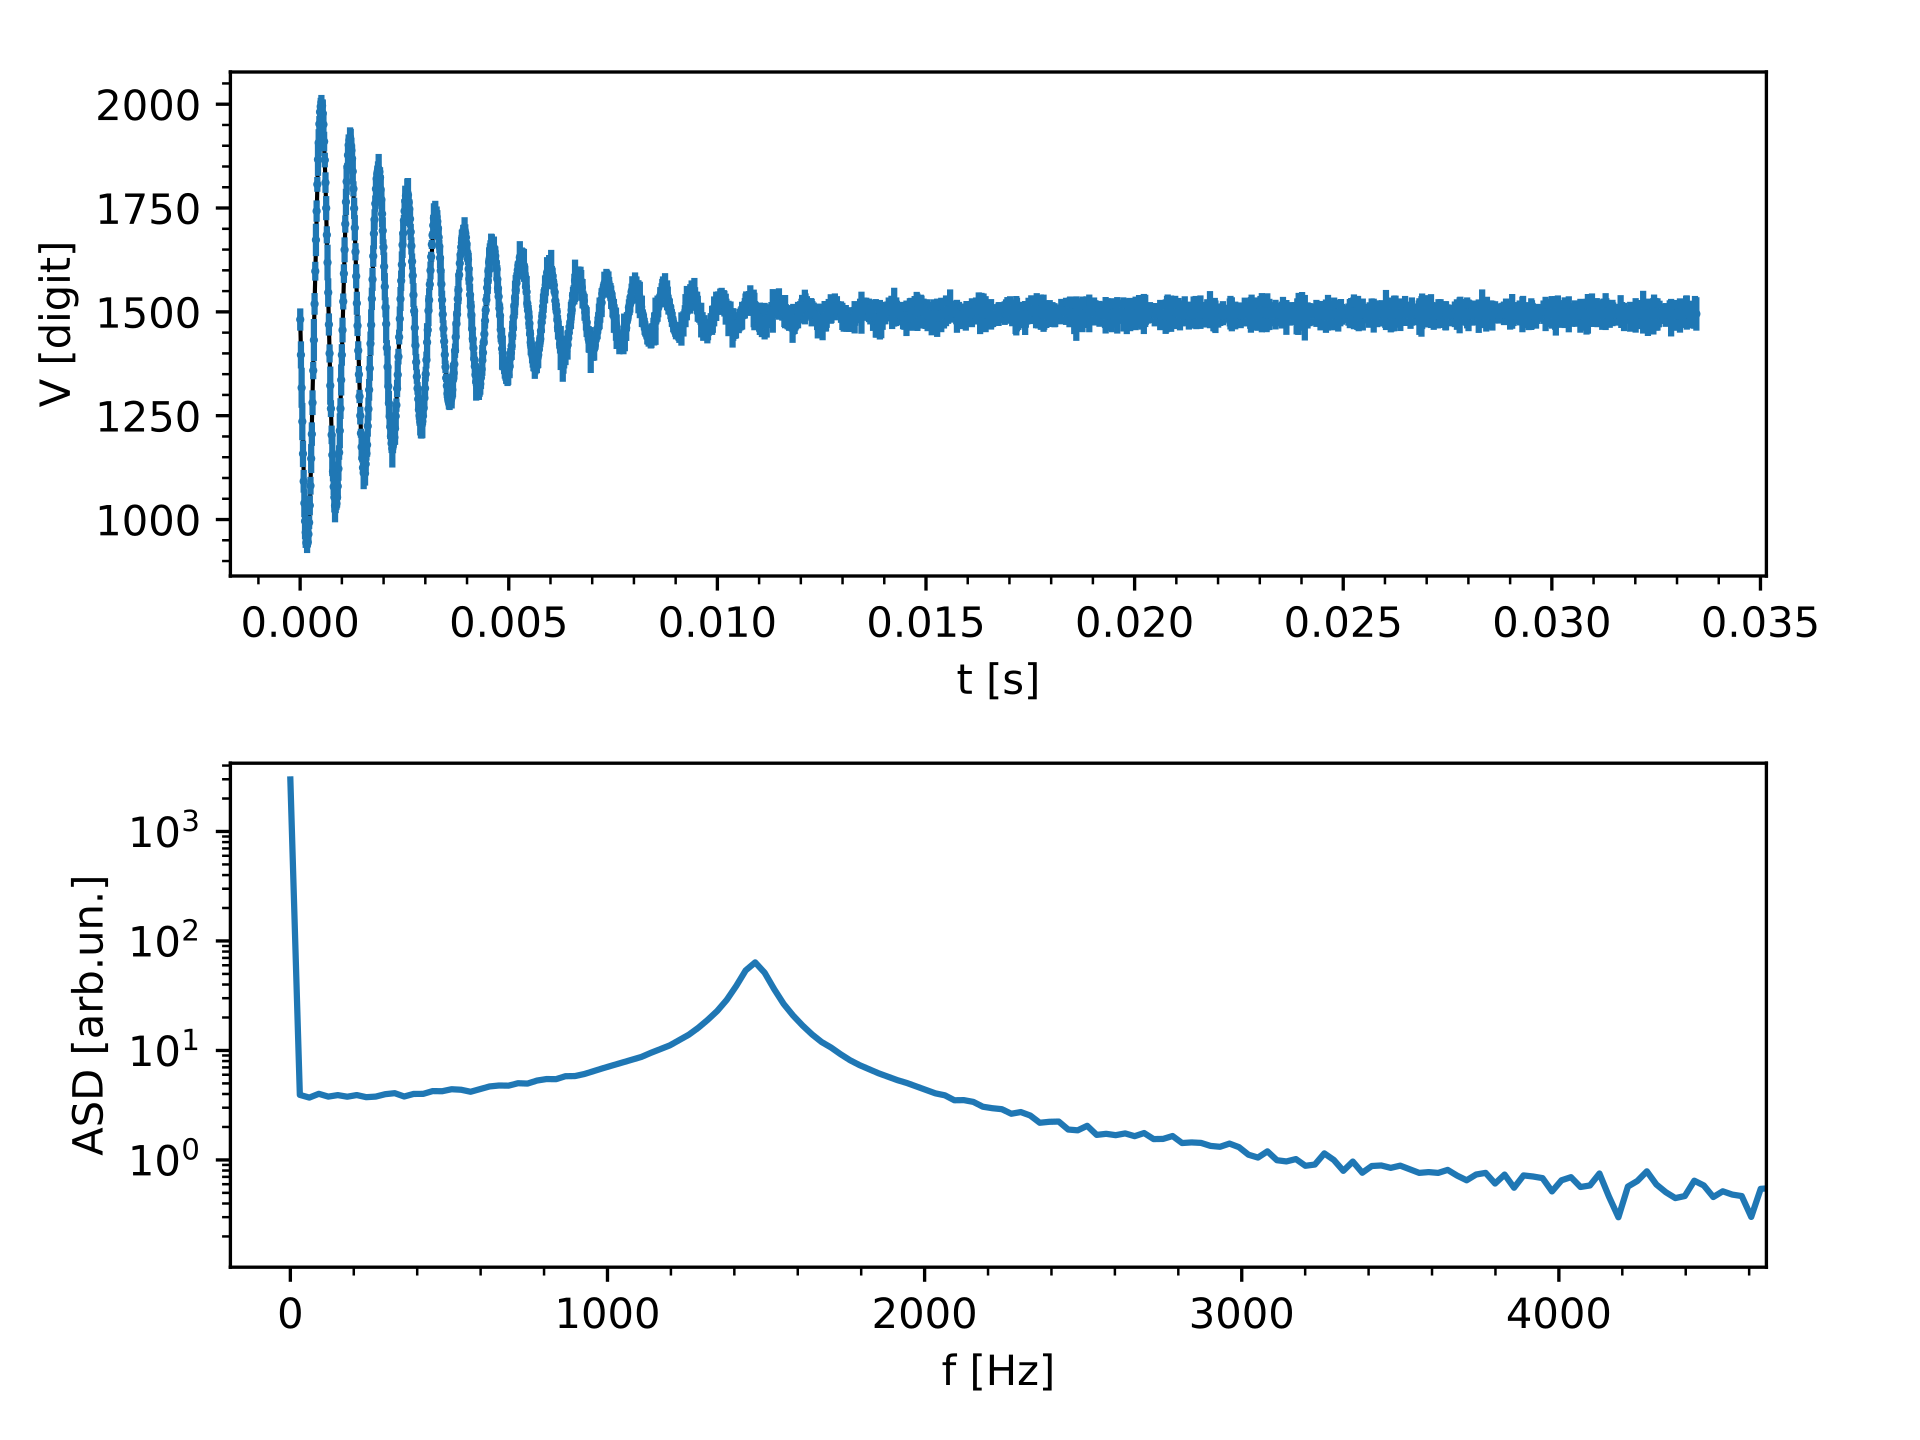
\includegraphics[width=0.50\columnwidth]{img/ese12/ind_antis.png}
    \caption{Dati e zoom della FFT, per diverse condizioni sperimentali. Da sinistra a destra: induttanza in parallelo, induttanza in anti-parallelo, induttanza in anti-serie.}
    \label{fig:ese12 - Induttanze in parallelo, antiparallelo e antiserie}
\end{figure}

\begin{figure}[H]
    \centering
    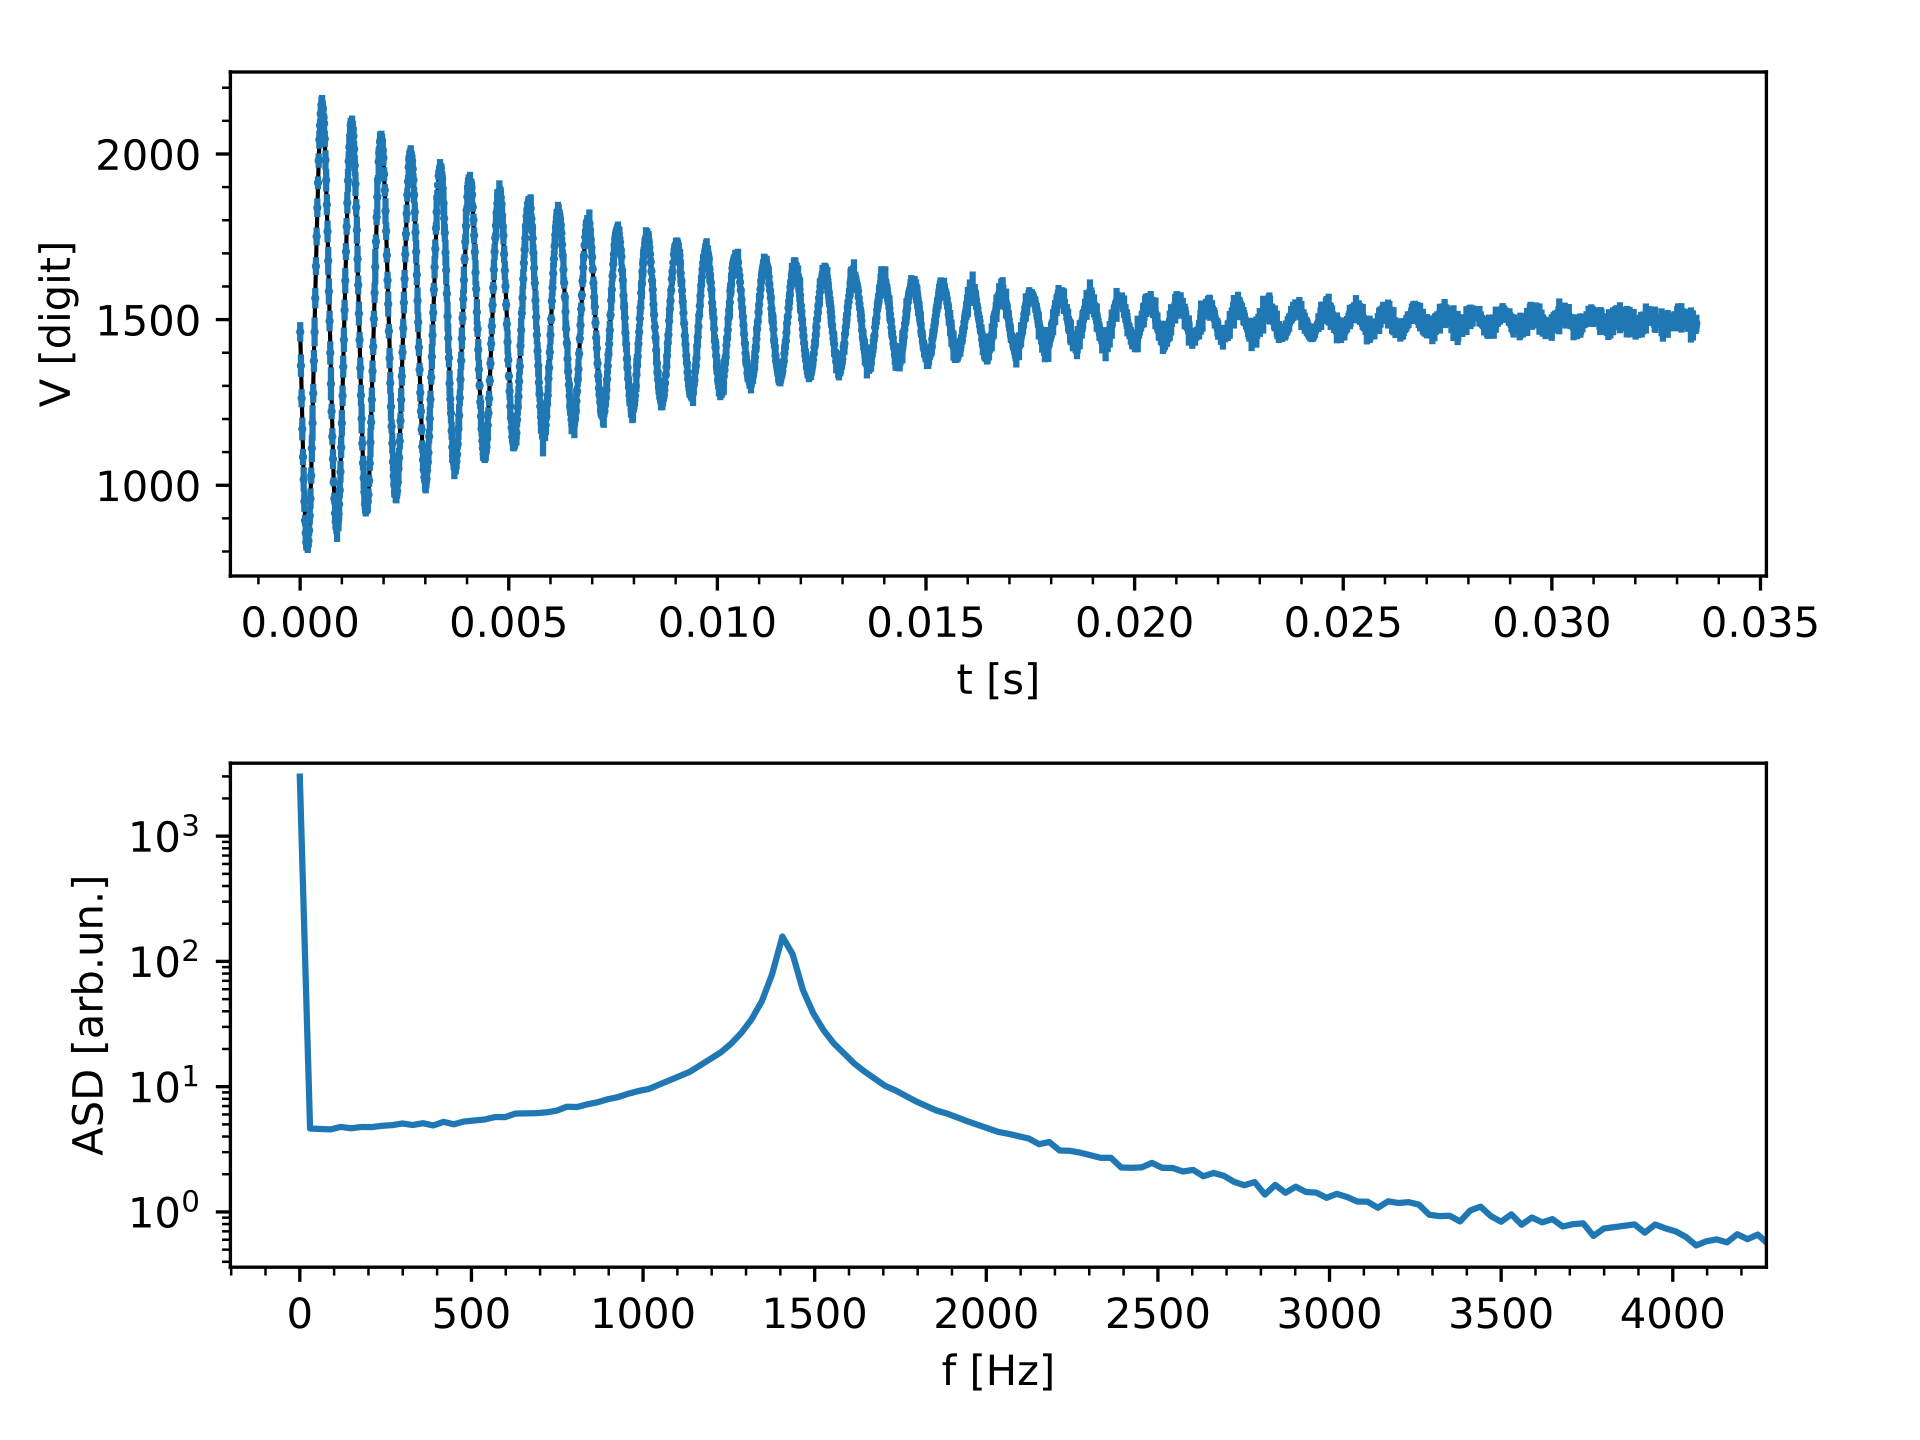
\includegraphics[width=0.48\columnwidth]{img/ese12/ind_int.png}
    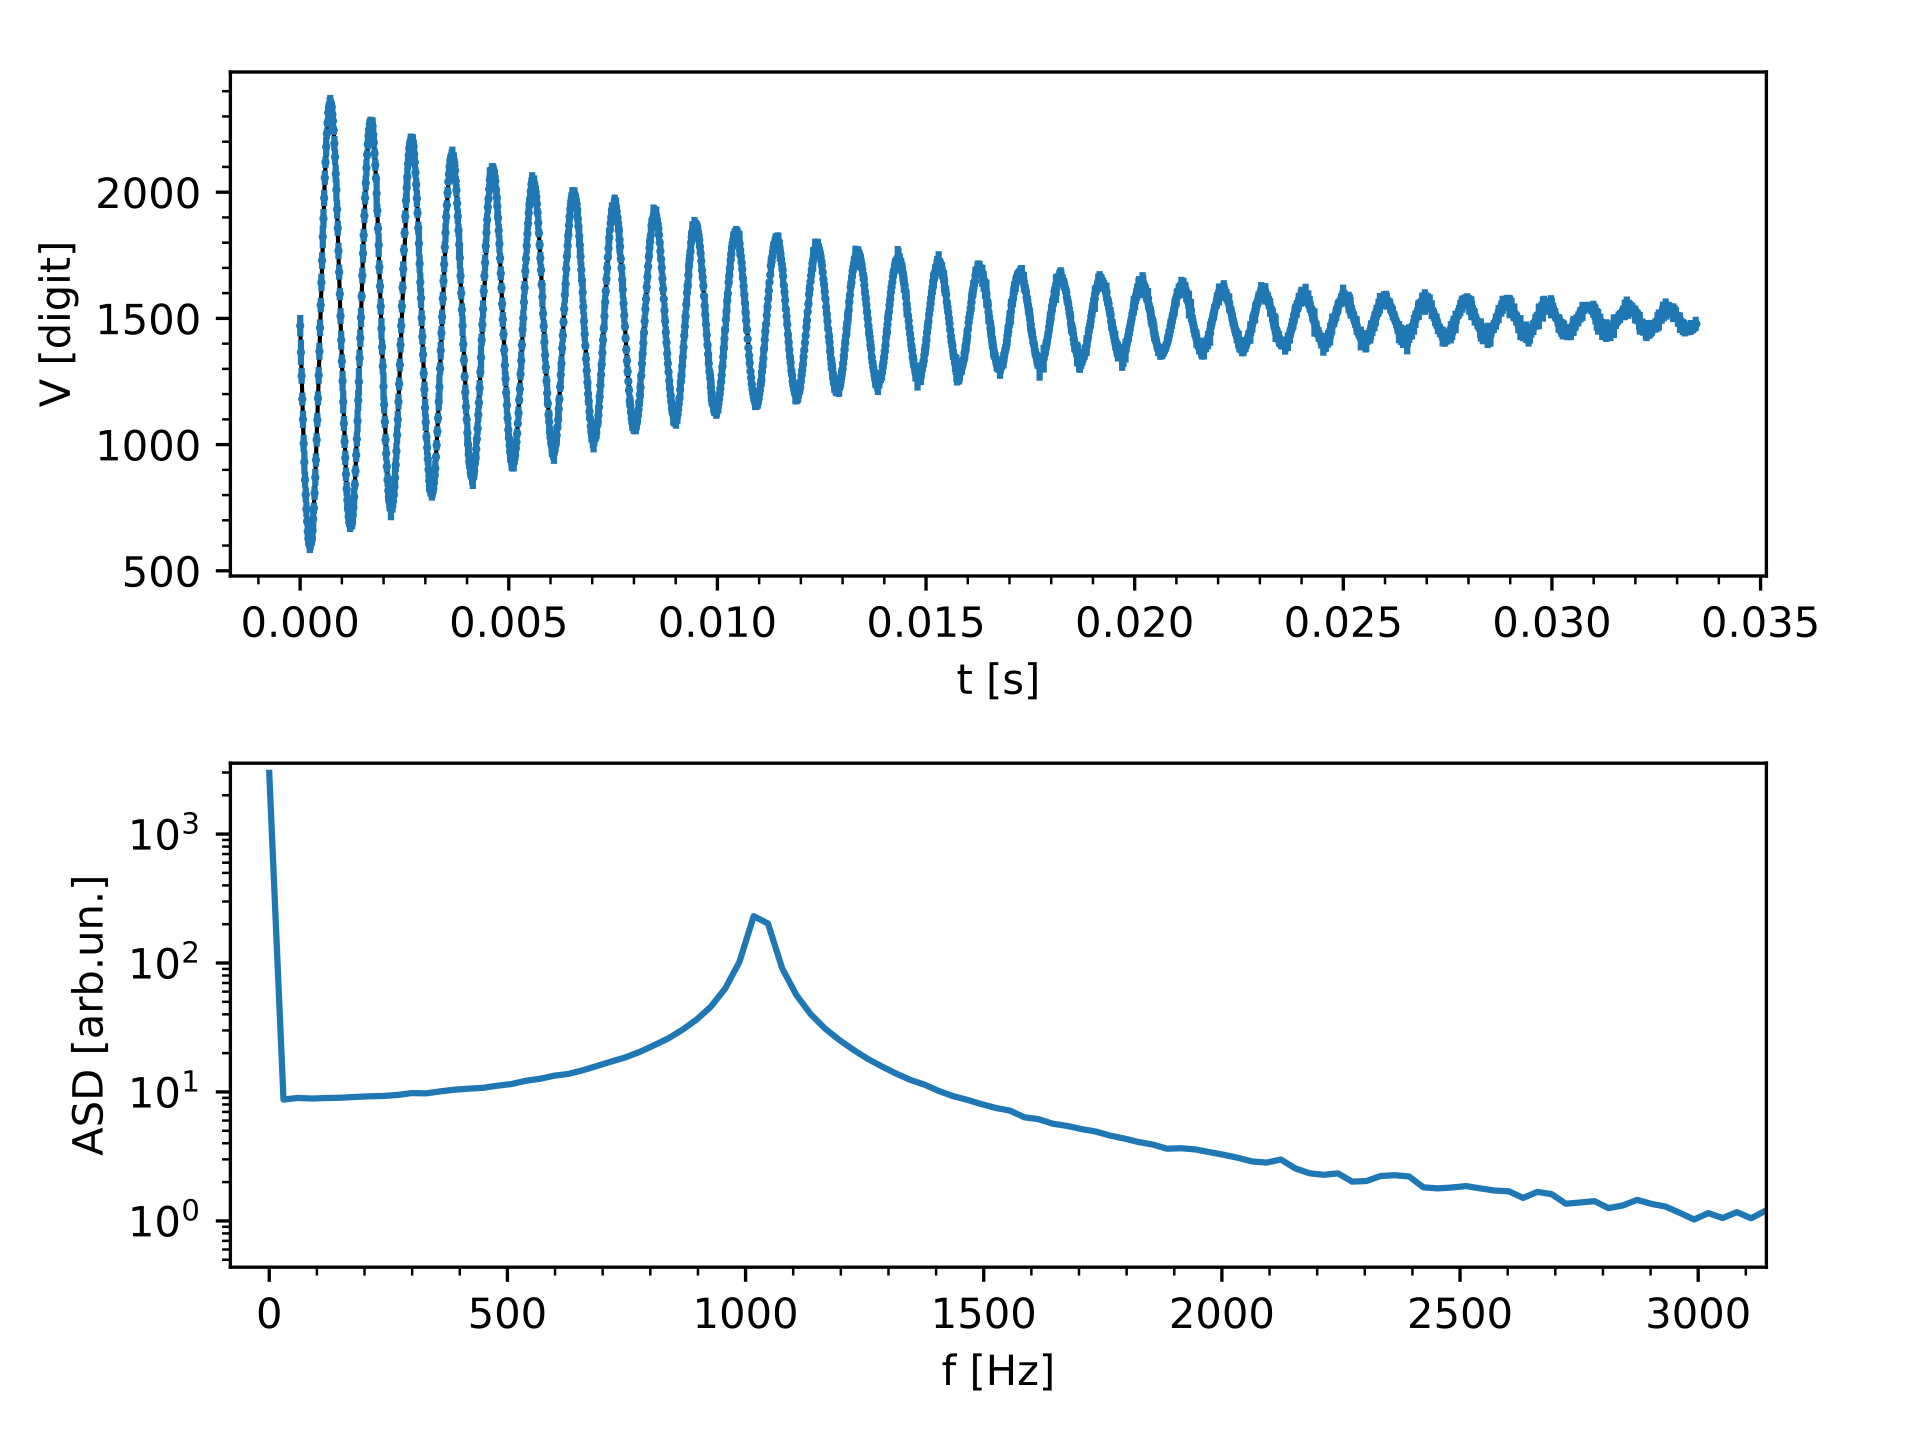
\includegraphics[width=0.48\columnwidth]{img/ese12/ind_est.png}
    \caption{Dati e zoom della FFT, questa volta utilizzando solo l'avvolgimento interno (sinistra) e poi solo quello esterno (destra).}
    \label{fig:ese12 - Induttanza avvolgimente interno ed esterno}
\end{figure}

\section{Correnti parassite}
In questa esperienza abbiamo realizzato un oscillatore RLC smorzato con lo stesso induttore della sezione precedente e un condensatore di capacità nominale $C = $($0.1  \pm 10 \%$) $\mu$F. Come nella sezione precedente, abbiamo misurato la d.d.p. ai capi del condensatore, stavolta inserendo diversi materiali fra gli avvolgimenti dell'induttore.\\
I grafici di seguito sono relativi a set di dati che spaziano tutti i possibili comportamenti. Analogamente alla sezione precedente, riportiamo una tabella con i valori di $T$ e $\tau$ ottenuti dal grafico della FFT confrontati con quelli ottenuti dal best-fit eseguito in laboratorio.\\

\begin{center}
    \begin{tabular}{|c||c|c||c|c|}
    \hline
        Oggetto & $T$ da FFT & $T$ da fit & $\tau$ da FFT & $\tau$ da fit\\
    \hline\hline
        Niente & 1.54 ms & (1.561102 $\pm$ 0.000008) ms & (13 $\pm$ 4) ms & (17.188 $\pm$ 0.005) ms\\
    \hline
        Alluminio profilato  & \multirow{2}{*}{1.60 ms} & \multirow{2}{*}{(1.557764 $\pm$ 0.000008) ms} & \multirow{2}{*}{(5 $\pm$ 4) ms} & \multirow{2}{*}{(14.582 $\pm$ 0.004) ms}\\
        segato con ferro pieno & & & &\\
    \hline
        Ferro laminato & 2.77 ms & (2.7688 $\pm$ 0.0005) ms & (15.9 $\pm$ 0.3) ms & (15.9 $\pm$ 0.1) ms\\
    \hline
        Ottone con ferro pieno & 1.51 ms & (1.511 $\pm$ 0.002) ms & (1.5 $\pm$ 0.1) ms & (1.51 $\pm$ 0.01) ms\\
    \hline
    \end{tabular}
\end{center}
Come per le tabelle della sezione precedente, notiamo accordo fra i valori ottenuti dai grafici delle FFT e dai fit, eccetto che per l'alluminio profilato, per il quale ci aspettavamo di trovare disaccordo in quanto la risoluzione delle frequenze è più bassa e il picco è molto vicino allo 0, per cui è fortemente asimmetrico. In questo caso non vale più la relazione che lega $\tau$ e $\Delta f_{\text{fwhm}}$.

\begin{figure}[H]
    \centering
    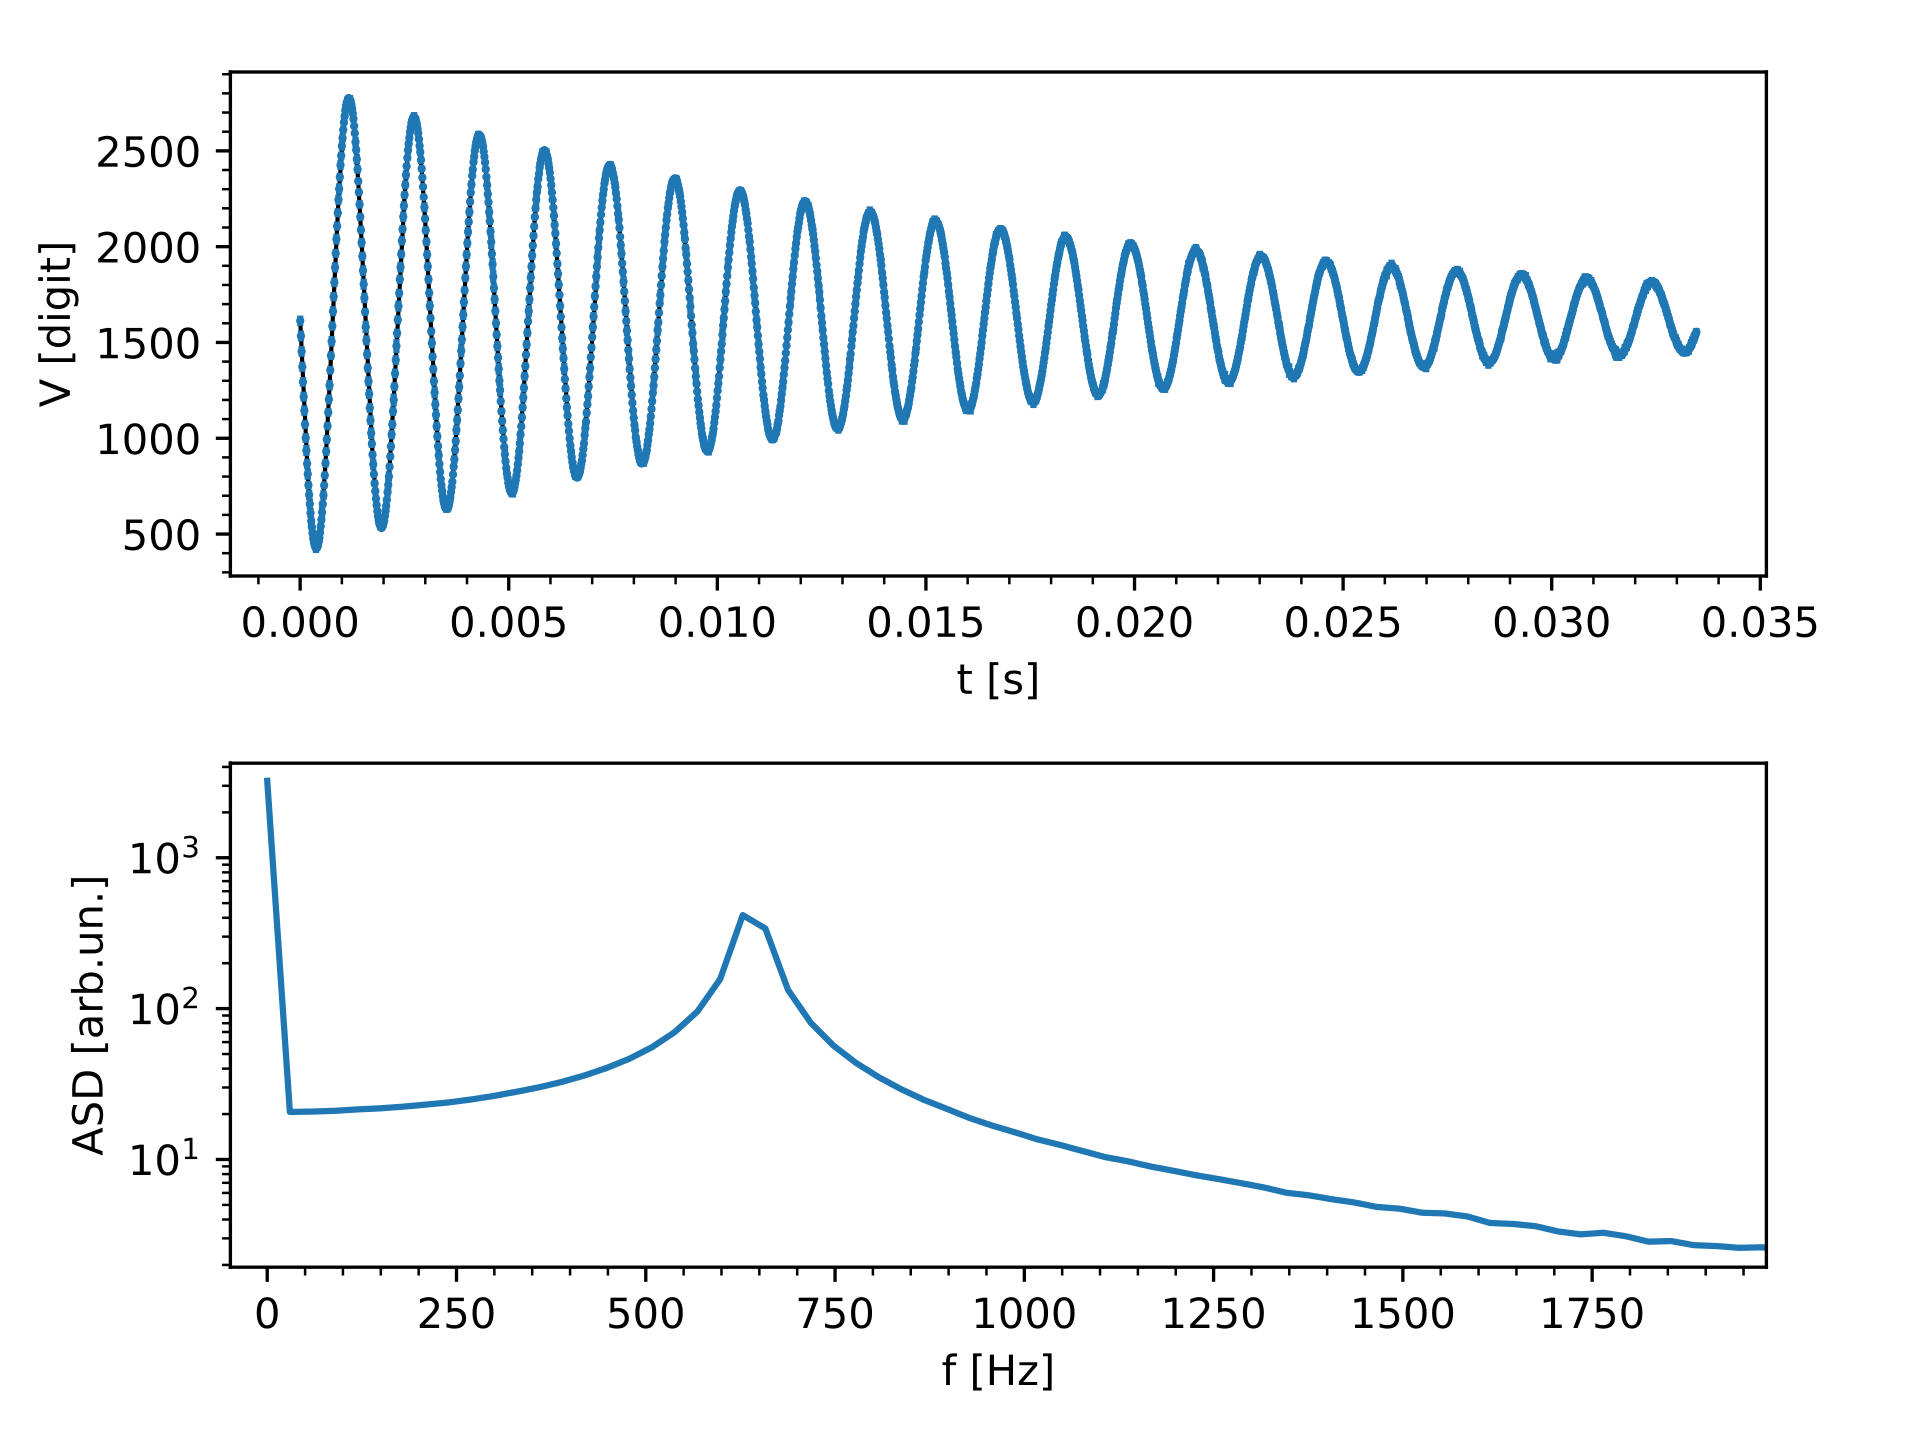
\includegraphics[width=0.48\columnwidth]{img/ese13/niente.png}    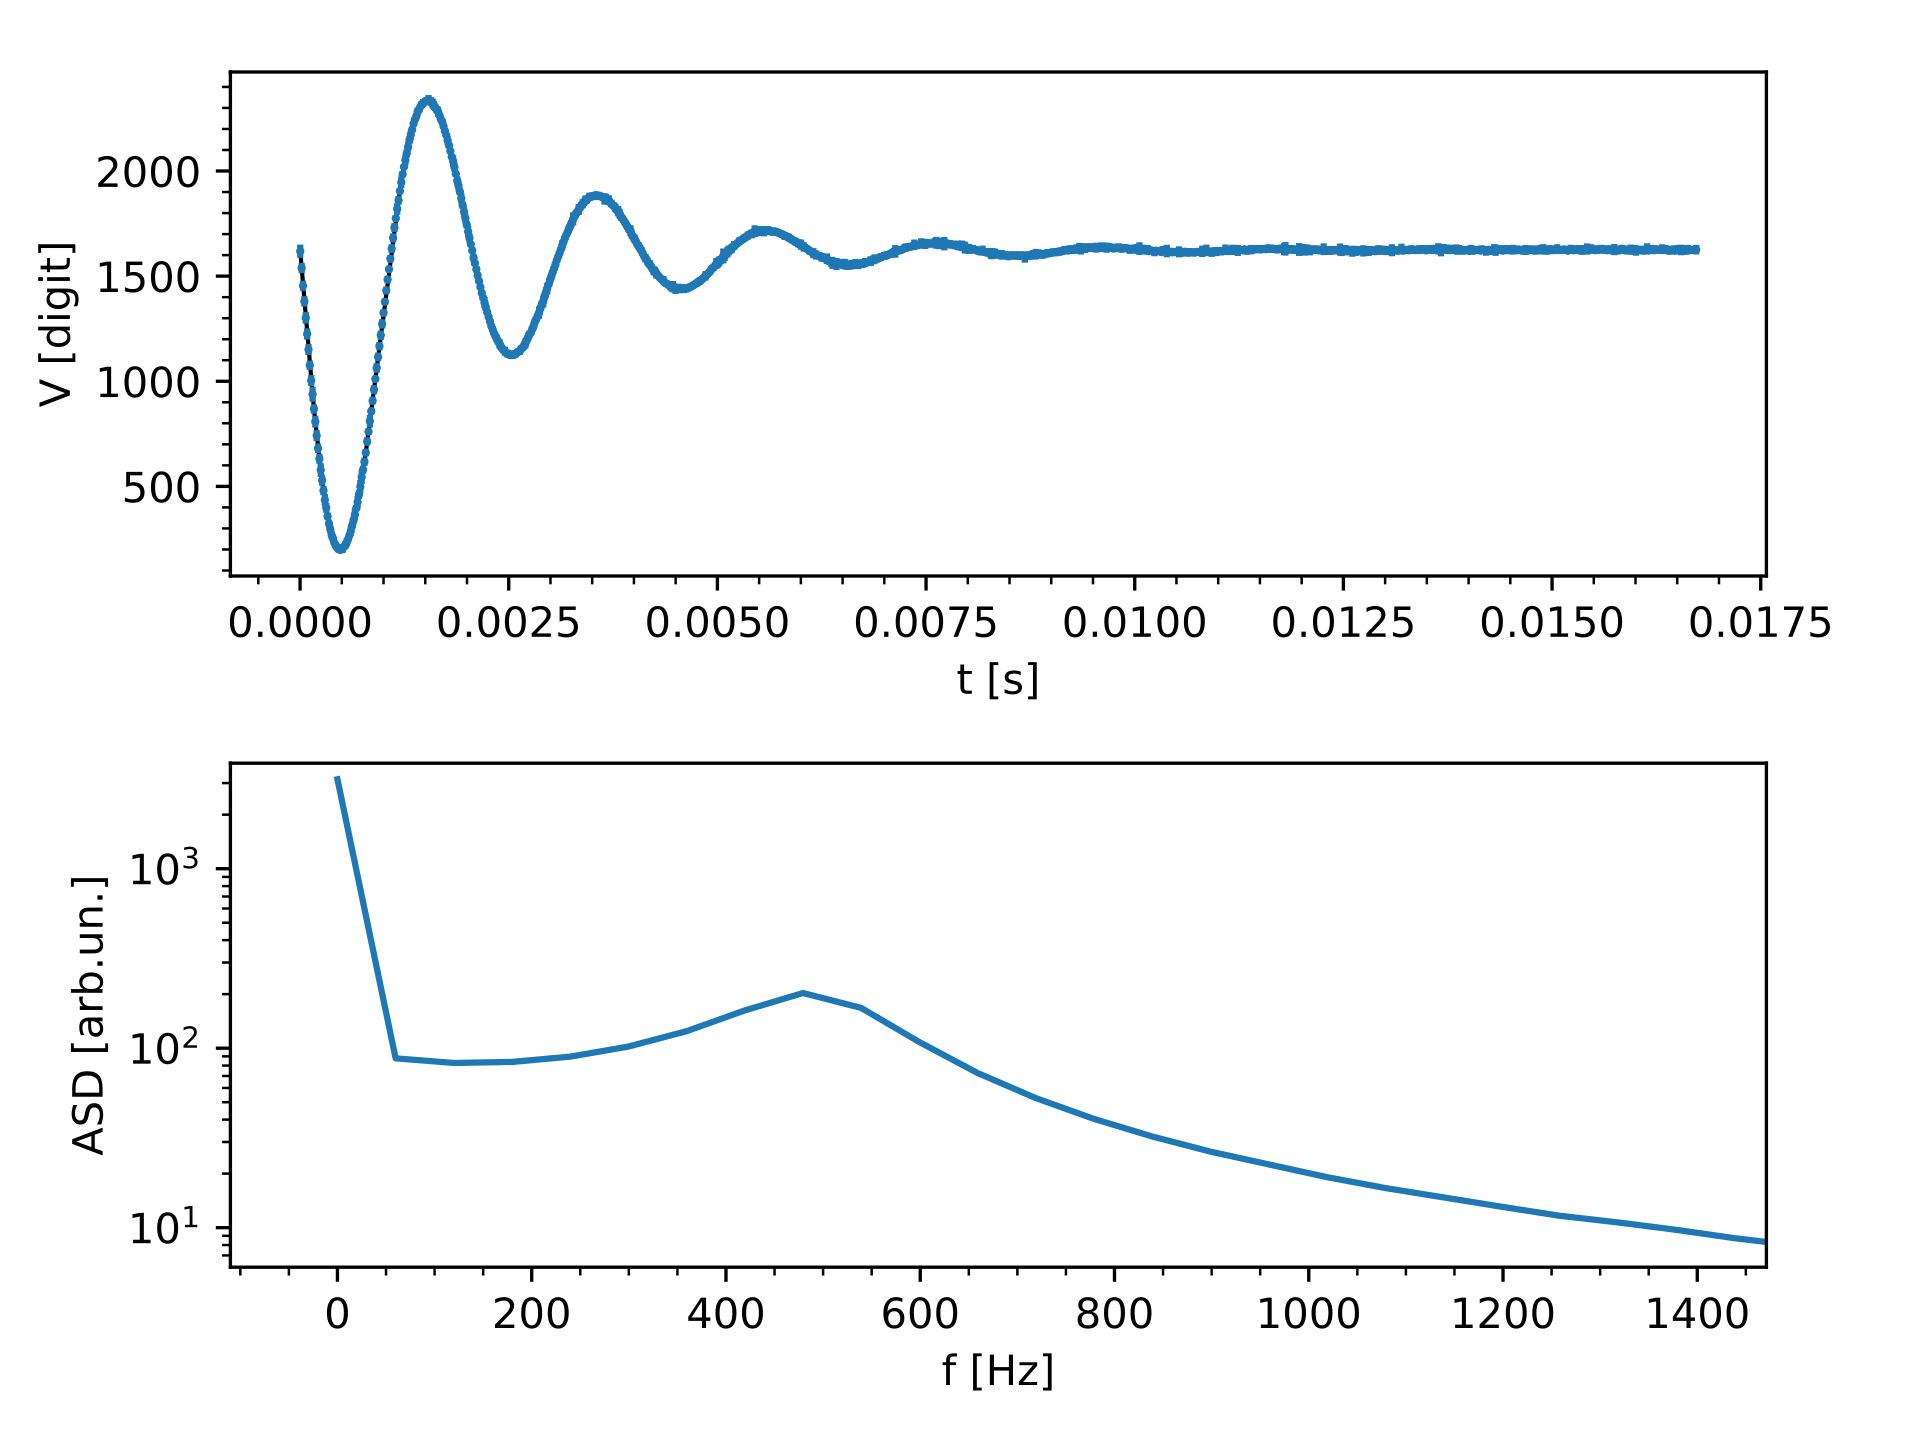
\includegraphics[width=0.48\columnwidth]{img/ese13/allsegferrpien.png}
    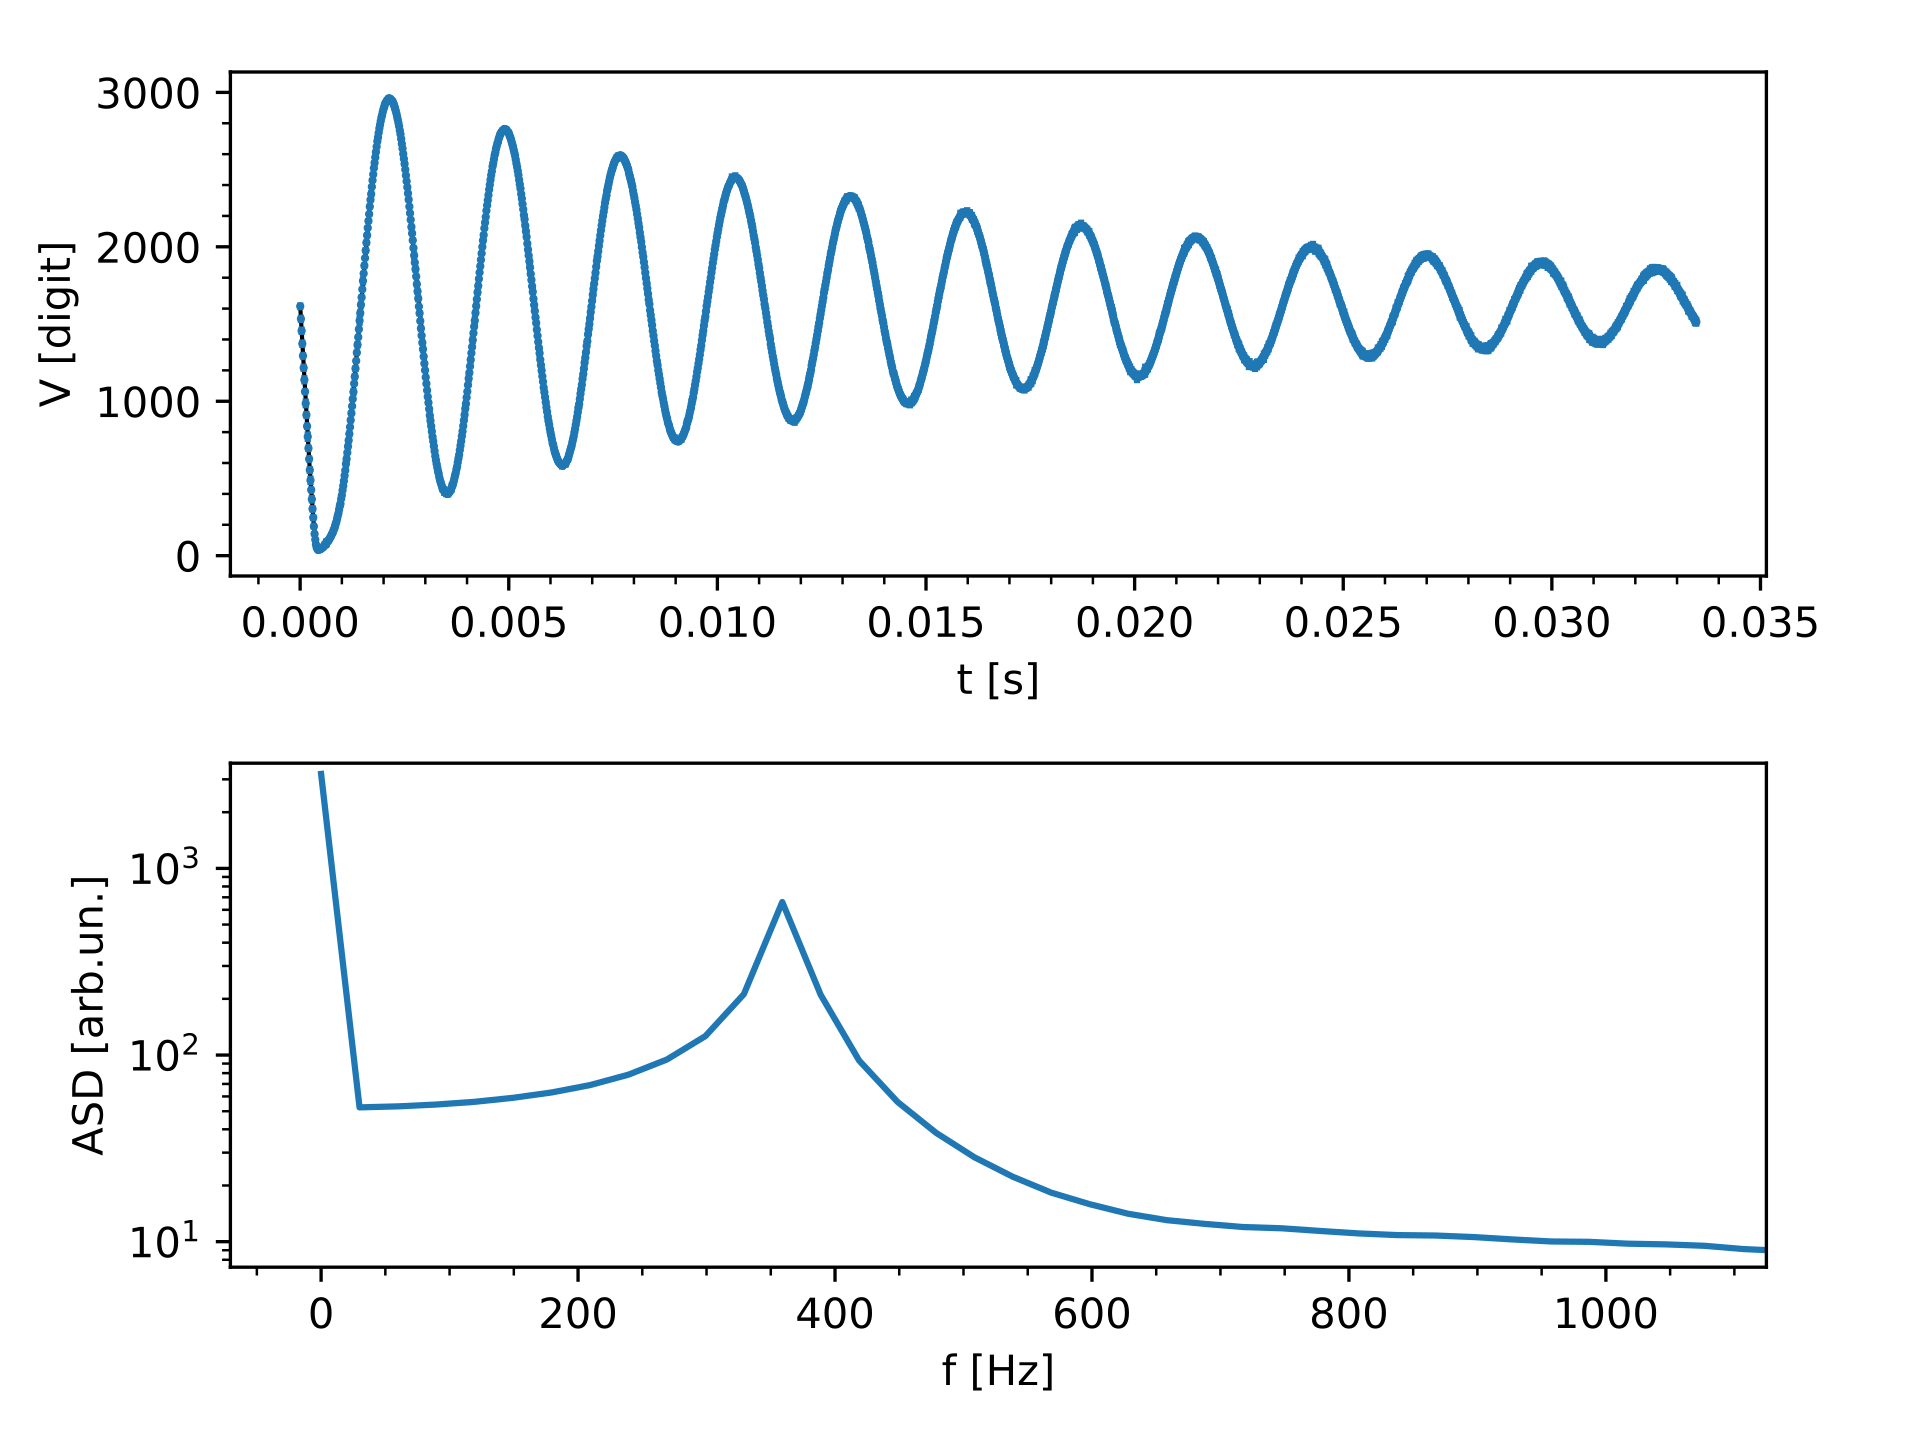
\includegraphics[width=0.48\columnwidth]{img/ese13/ferrlam.png}
    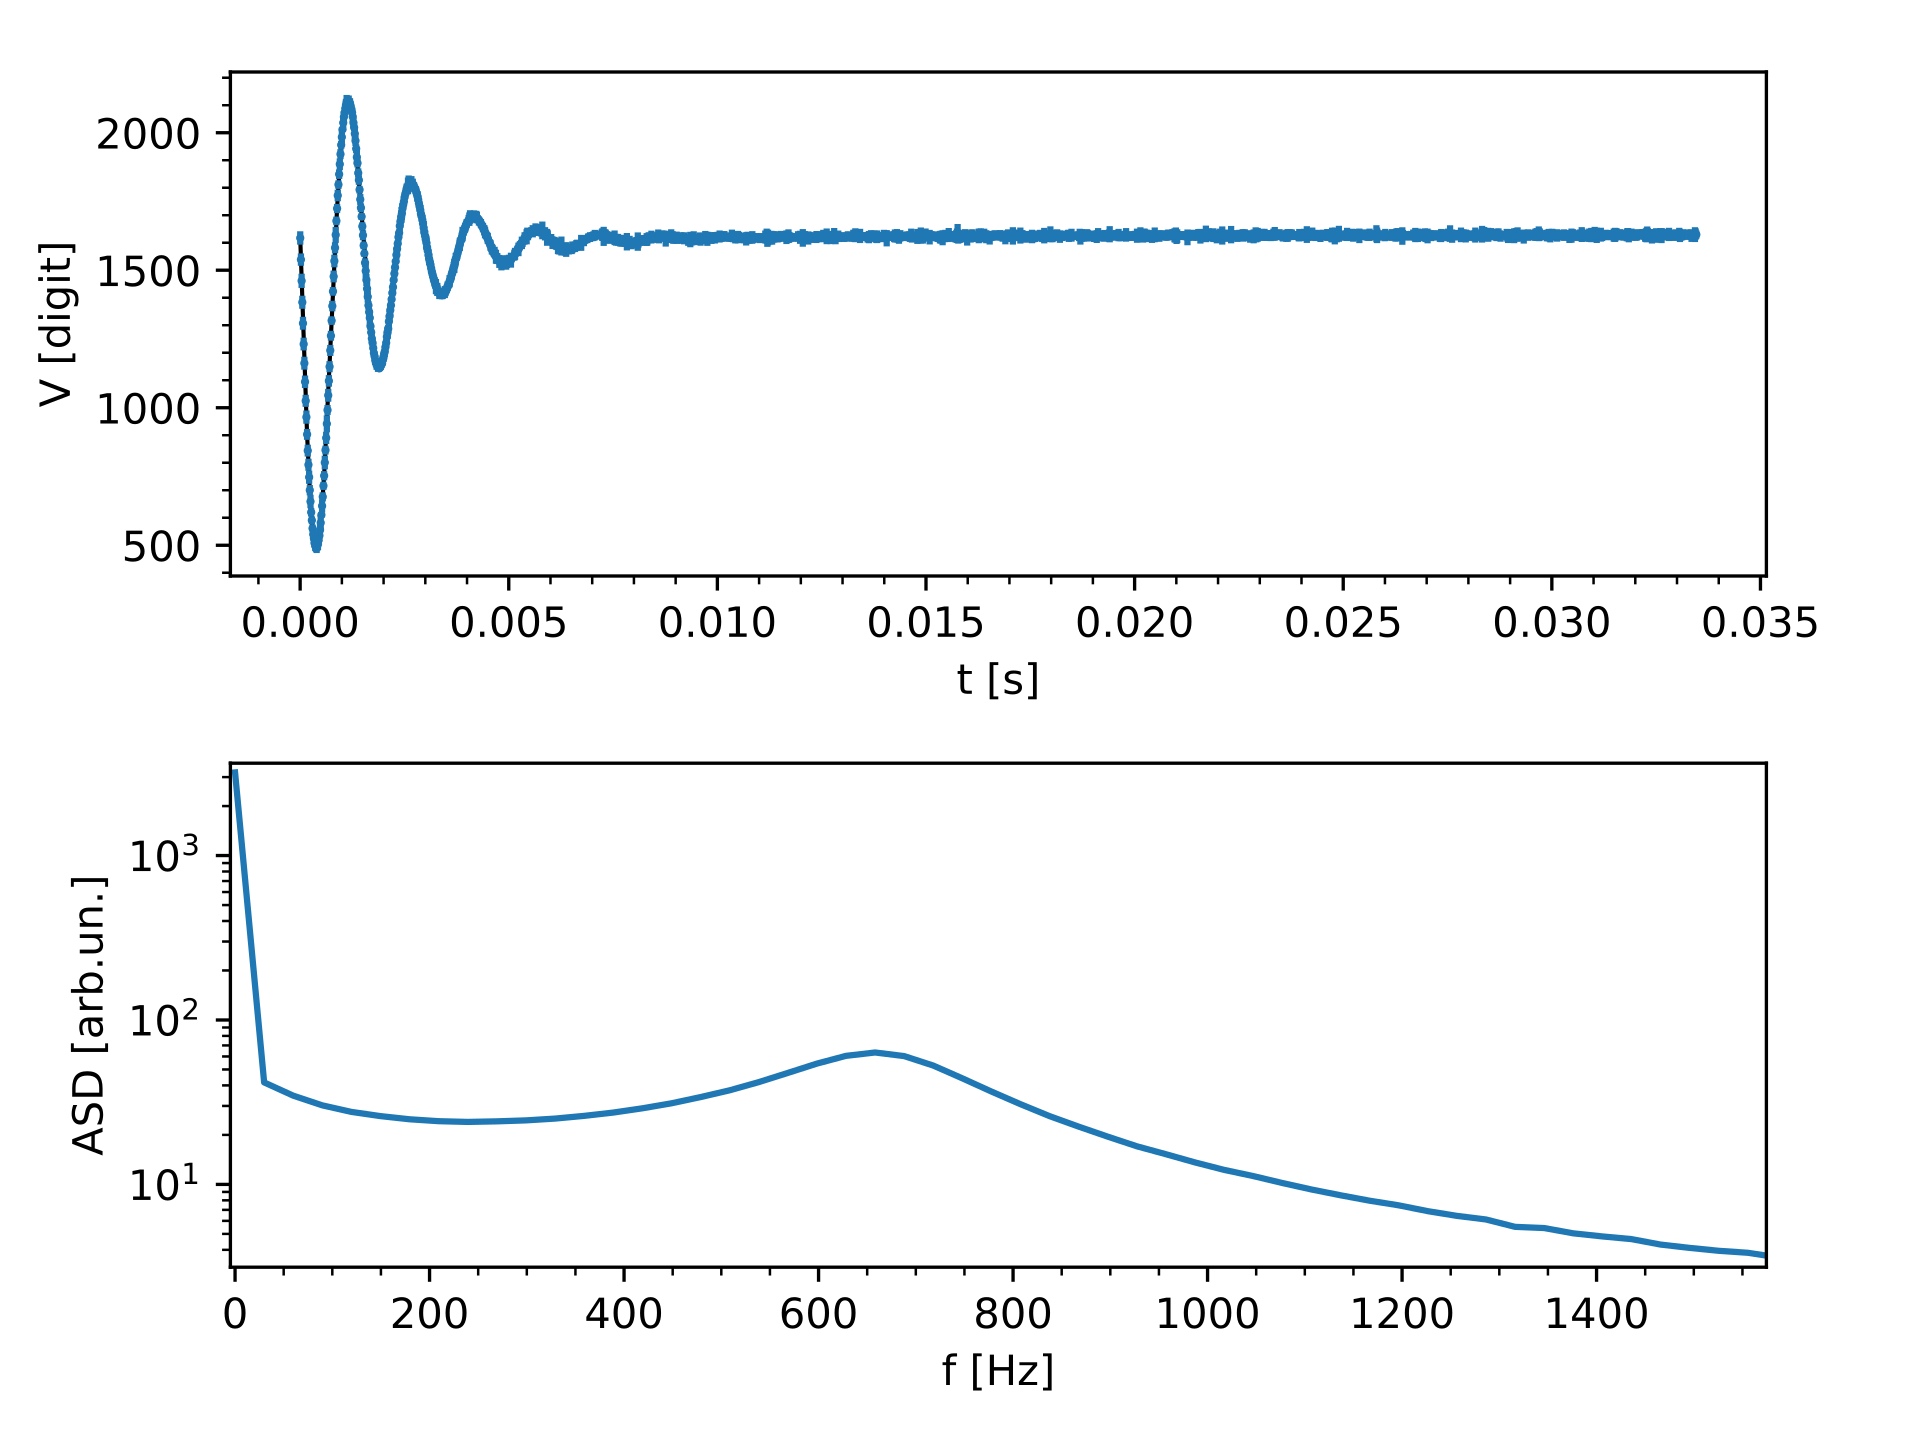
\includegraphics[width=0.48\columnwidth]{img/ese13/ottferrpien.png}
    \caption{Grafici relativi a circuiti RLC con diversi materiali all'interno del nucleo dell'induttore. Da sinistra a destra: niente, alluminio profilato segato per lungo con ferro pieno, ferro laminato, ottone con ferro pieno.}
    \label{fig:ese13 corrrenti parassite}
\end{figure}


\end{document}

